%\documentclass[defaultstyle,12pt,master,Helvetica]{01.thesis}
\documentclass[defaultstyle,12pt,master]{01.thesis}
% Helvetica is a similar font to Arial, with small differences.

%% Packages
% Defines an additional alphabet... not required in most cases
% ------------------------------------------------------------
% \DeclareMathAlphabet{\mathpzc}{OT1}{pzc}{m}{it}

% PACKAGE babel:
% ---------------
% The 'babel' package may correct some hyphenisation issues of latex. 
% However in most situations it is not required.
\usepackage[portuguese]{babel}

% PACKAGE fontenc:
% -----------------
% chooses T1-fonts and allows correct automatic hyphenation.
\usepackage[T1]{fontenc}
%\usepackage[utf8]{inputenc}
%%NEW
\usepackage{fontspec}
\setmainfont{Calibri}
%%END
% Package ulem.
\usepackage{ulem} % Allows the use of other text emphatizer commands
\normalem %defines \emph{} to italic, instead of underline. 
\raggedbottom %declaration makes all pages the height of the text on that page. No extra vertical space is added. The \flushbottom declaration makes all text pages the same height, adding extra vertical space when necessary to fill out the page.

% PACKAGE date time:
% -----------------
% Lets you alter the format of the date that \today returns.
\usepackage{datetime}
\newdateformat{todaythesis}{%
\monthname[\THEMONTH]  \THEYEAR}

% PACKAGE latexsym:
% -----------------
% Defines additional latex symbols. May be required for thesis with many math symbols.
\usepackage{latexsym}

% PACKAGE amsmath, amsthm, amssymb, amsfonts:
% -------------------------------------------
% This package is typically required. Among many other things it adds the possibility
% to put symbols in bold by using \boldsymbol (not \mathbf); defines additional 
% fonts and symbols; adds the \eqref command for citing equations. I prefer the style
% "(x.xx)" for referering to an equation than to use "equation x.xx".
\usepackage{amsmath, amsthm, amssymb, amsfonts, amsbsy}

% PACKAGE multirow, colortbl, longtable:
% ---------------------------------------
% These packages are most usefull for advanced tables. The first allows to join rows 
% throuhg the command \multirow which works similarly with the command \multicolumn
% The second package allows to color the table (both foreground and background)
% The third package is only required when tables extend beyond the length of one page;
% with compatibilities with the tabular environment. The last allow the definitions of landscape pages, allowing the use of a different orientation for wider graphics or tables. See package documentation to see the implementation.
\usepackage{multirow}
\usepackage{colortbl}
\usepackage{supertabular}
\usepackage{pdflscape}
% \usepackage{longtable}

% PACKAGE graphics, epsfig, subfigure, caption:
% ---------------------------------------------
% Packages for figures... well you will certainly need these packages, with the exception
% of the 'caption' package. This only allows to define extra caption options.
% Notice that subfigure allows to place figures within figures with its own caption. It
% should be avoided to create an eps file with subfigures. That will mean that you won't be 
% able to reference those subfigures. Instead create an EPS file (the only graphics format supported
% by latex) for each of the subfigures and then use the command \subfigure (see below).
\usepackage{graphics}
\usepackage{graphicx}
\usepackage{epsfig}
\usepackage[hang,small,bf]{subfigure}
%\usepackage[footnotesize,bf,center]{caption}
\usepackage{dcolumn}
\usepackage{bm}
\usepackage{booktabs}
\usepackage{rotating}
\usepackage{multirow}

\usepackage[font=small,labelfont=bf,textfont=normalfont,labelsep=endash]{caption}

% PACKAGE algorithmic, algorithm
% ------------------------------
% These packages are required if you need to describe an algorithm.
\usepackage[chapter, boxed]{algorithm}
%\usepackage{algorithmic}
\usepackage{algpseudocode}
\renewcommand*\Call[2]{\textproc{#1}(#2)}
% PACKAGE natbib/cite
% -------------------
% The two packages are not compatible, and you should use one of the two. Notice however that the
% IEEE BiBTeX stylesheet is imcompatible with the natbib package. If using the IEEE format, use the 
% cite package instead
%\usepackage[square,numbers,sort&compress]{natbib}
\usepackage[sort&compress]{natbib}
%\usepackage{cite}

% PACKAGE acronyum
% -----------------
% This package is most useful for acronyms. The package guarantees that all acronyms definitions are 
% given at the first usage. IMPORTANT: do not use acronyms in titles/captions; otherwise the definition 
% will appear on the table of contents.
\usepackage[printonlyused]{acronym}
\usepackage[titletoc,title,header]{appendix}
\usepackage[noauto]{chappg}

% PACKAGE extra_functions VER COMO DEVE SER
% -----------------
% My Personal package: defines the following commands:
% \fancychapter{chaptername) -> Prints a fancier chapter (you can also use the fancychapter package for this)
% \hline{width} -> use for a replacement of the \hline command
% \Mark1, \Mark2, \Mark3, ...
\usepackage{00.extra_functions}


% PACKAGE hyperref
% -----------------
% Set links for references and citations in document
% Some MiKTeX distributions have faulty PDF creators in which case this package will not work correctly
% Long live Linux :D
%\usepackage[plainpages=false]{hyperref}
\usepackage[plainpages=false,unicode]{hyperref}
\hypersetup{
             colorlinks=false,
             citecolor=red,
             breaklinks=true,
             bookmarksnumbered=true,
             bookmarksopen=true,
             pdftitle={Programção genética aplicada a previsão de parâmetros farmacocinéticos e a previsão do ano de lançamento de músicas},
             pdfauthor={Dizando Norton},
             pdfsubject={Mestrado em Gestão de Informação},
             pdfcreator={Dizando Norton},
             pdfkeywords={Latex, Mestrado}}
\usepackage{float}
%\usepackage[final]{00.listofsymbols}
\usepackage{00.symlist}

% Set paragraph counter to alphanumeric mode
\renewcommand{\theparagraph}{\Alph{paragraph}~--}

\newcommand{\figref}[1]{Figura \ref{#1}}
\newcommand{\equationref}[1]{Equação (\ref{#1})}
\newcommand{\tableref}[1]{Tabela \ref{#1}}
\newcommand{\algreff}[1]{Algoritmo \ref{#1}}
% Algorithm customization
\floatname{algorithm}{Algoritmo}
\algrenewcommand{\algorithmicrequire}{\textbf{entrada:}}
\algrenewcommand{\algorithmicensure}{\textbf{saída:}}
\algrenewcommand{\algorithmicend}{\textbf{fim}}
\algrenewcommand{\algorithmicif}{\textbf{se}}
\algrenewcommand{\algorithmicthen}{\textbf{então}}
\algrenewcommand{\algorithmicelse}{\textbf{senão}}
%\algrenewcommand{\algorithmicelsif}{\algorithmicelse\ \algorithmicif}
%\algrenewcommand{\algorithmicendif}{\algorithmicend\ \algorithmicif}
\algrenewcommand{\algorithmicfor}{\textbf{para}}
\algrenewcommand{\algorithmicforall}{\textbf{para todos}}
\algrenewcommand{\algorithmicdo}{\textbf{fa\c{c}a}}
%\algrenewcommand{\algorithmicendfor}{\algorithmicend\ \algorithmicfor}
\algrenewcommand{\algorithmicwhile}{\textbf{enquanto}}
%\algrenewcommand{\algorithmicendwhile}{\algorithmicend\ \algorithmicwhile}
\algrenewcommand{\algorithmicloop}{\textbf{loop}}
%\algrenewcommand{\algorithmicendloop}{\algorithmicend\ \algorithmicloop}
\algrenewcommand{\algorithmicrepeat}{\textbf{repita}}
\algrenewcommand{\algorithmicuntil}{\textbf{at\acute{e}}}
%\algrenewcommand{\algorithmicprint}{\textbf{imprima}}
\algrenewcommand{\algorithmicreturn}{\textbf{retorne}}
%\algrenewcommand{\algorithmictrue}{\textbf{verdadeiro}}
%\algrenewcommand{\algorithmicfalse}{\textbf{falso}}
\algrenewcommand{\algorithmicrequire}{\textbf{entrada:}}
\algrenewcommand{\algorithmicensure}{\textbf{saída:}}
\algrenewcommand{\algorithmicfunction}{\textbf{função}}
%Of algorithms customization

\newcommand{\textreg}{$\textsuperscript{\textregistered}$}

\usepackage{pdfpages}
%\usepackage[onehalfspacing]{setspace}

%\setstretch{2}
\usepackage{qtree}

\usepackage{tikz}
\usetikzlibrary{arrows}
%\usepackage{tikz-qtree}
\usepackage{pgfkeys}
\usepackage{pgfplots}
\usetikzlibrary{pgfplots.statistics}
\usepackage{pgfplotstable}
\pgfplotsset{compat=1.5}
\usepackage{pgf-pie}
\usepackage{filecontents}
%\usepackage{subcaption}
\usepackage{gnuplottex}
\usepackage{graphicx}
\usepackage{latexsym}
\usepackage{keyval}
\usepackage{moreverb}
%\usepackage[round-precision=2]{siunitx}
%\%sisetup{round-mode=places,round-precision=3}
%\usepackage{gnuplot}
\usepgfplotslibrary{external}
\usepgfplotslibrary{groupplots}
\tikzexternalize

%algoritmos
%\usepackage[]{algorithm2e}

%\usepackage{draftwatermark}
%\SetWatermarkFontSize{1cm}
%\SetWatermarkScale{4}
%\SetWatermarkLightness{0.9}
%\SetWatermarkText{Rascunho}

%teste de graficos
\usepackage{tikz}
\usetikzlibrary{decorations.text,shadows}
\usepackage{ifthen}
\usepackage{bchart}
\usepackage{pdflscape}
\usepackage{forest}
\usepackage[bottom]{footmisc}
\renewcommand{\labelitemi}{\scriptsize$\blacksquare$}	
\renewcommand{\bibname}{\large{BIBLIOGRAFIA}}
%\usepackage{apacite}

\usepackage{tocloft}
\renewcommand{\cftafterlottitle}{\hfill}
\renewcommand{\cftafterloftitle}{\hfill}
%% Page formatting
\hoffset 0in
\voffset 0in

%Alternative set of page geometry
%\oddsidemargin 0.71cm
%\evensidemargin 0.04cm
%\marginparsep 0in
%\topmargin -0.25cm
%\textwidth 15cm
%\textheight 23.5cm
\usepackage{titlesec}

\titleformat*{\section}{\large\bfseries}
\titlelabel{\thetitle.\quad}
\let \savenumberline \numberline
\def \numberline#1{\savenumberline{#1.}}
% OLD VERSION \usepackage[top=2.5cm, bottom=2.5cm, inner=2.9cm, outer=2.5cm]{geometry}
%ISEGI NUMBERS
\usepackage[top=3.5cm, bottom=2.5cm, left=3.5cm, right=2.5cm]{geometry}
\usepackage{setspace}

\usepackage{fancyhdr}
\pagestyle{fancy}
\renewcommand{\contentsname}{Conteudo}
\renewcommand{\chaptermark}[1]{\markboth{\thechapter.\ #1}{}}
\renewcommand{\sectionmark}[1]{\markright{\small\thesection\ #1}}
\fancyhf{} 
%\fancyhead[LE]{\bfseries\nouppercase{\leftmark}}
%\fancyhead[RO]{\bfseries\nouppercase{\rightmark}}
\fancyfoot[LE,RO]{\bfseries\small\thepage}
\renewcommand{\headrulewidth}{0.0pt}
\renewcommand{\footrulewidth}{0.0pt}
\addtolength{\headheight}{2pt} % make space for the rule
\fancypagestyle{plain}{% Used in Chapter titles
   \fancyhead{} % get rid of headers
   \renewcommand{\headrulewidth}{0pt} % and the line
   \renewcommand{\footrulewidth}{0pt}
   \fancyfoot[LE,RO]{\bfseries\small\thepage}
}

\fancypagestyle{begin}{%
   \fancyhead{}
   \renewcommand{\headrulewidth}{0pt}
   \renewcommand{\footrulewidth}{0pt}
   \fancyfoot[LE,RO]{\bfseries\small\thepage}
}
\fancypagestyle{document}{%
	\fancyhf{} 
	\fancyhead[LE]{\bfseries\nouppercase{\leftmark}}
	\fancyhead[RO]{\bfseries\nouppercase{\rightmark}}
	\fancyfoot[LE,RO]{\bfseries\small\thepage}
	%\renewcommand{\headrulewidth}{0pt}
	%\renewcommand{\footrulewidth}{0pt}
	\addtolength{\headheight}{2pt} % make space for the rule
}
\fancypagestyle{documentsimple}{%
	\fancyhf{}
	\fancyfoot[LE,RO]{\bfseries\small\thepage}
	%\renewcommand{\headrulewidth}{0pt}
	%\renewcommand{\footrulewidth}{0pt}
	\addtolength{\headheight}{2pt} % make space for the rule
	\setlength{\parindent}{1cm}
	\setstretch{1.5}
}
\setcounter{secnumdepth} {5}
\setcounter{tocdepth} {5}
\renewcommand{\thesubsubsection}{\thesubsection.\Alph{subsubsection}}

\renewcommand{\subfigtopskip}{0.3 cm}
\renewcommand{\subfigbottomskip}{0.2 cm}
\renewcommand{\subfigcapskip}{0.3 cm}
\renewcommand{\subfigcapmargin}{0.2 cm}
\renewcommand{\mtctitle}{Conteúdo}
\graphicspath{{figures/}}


%-----------------------------------------------------------
%-----------------------------------------------------------
\begin{document}
\pagestyle{begin}
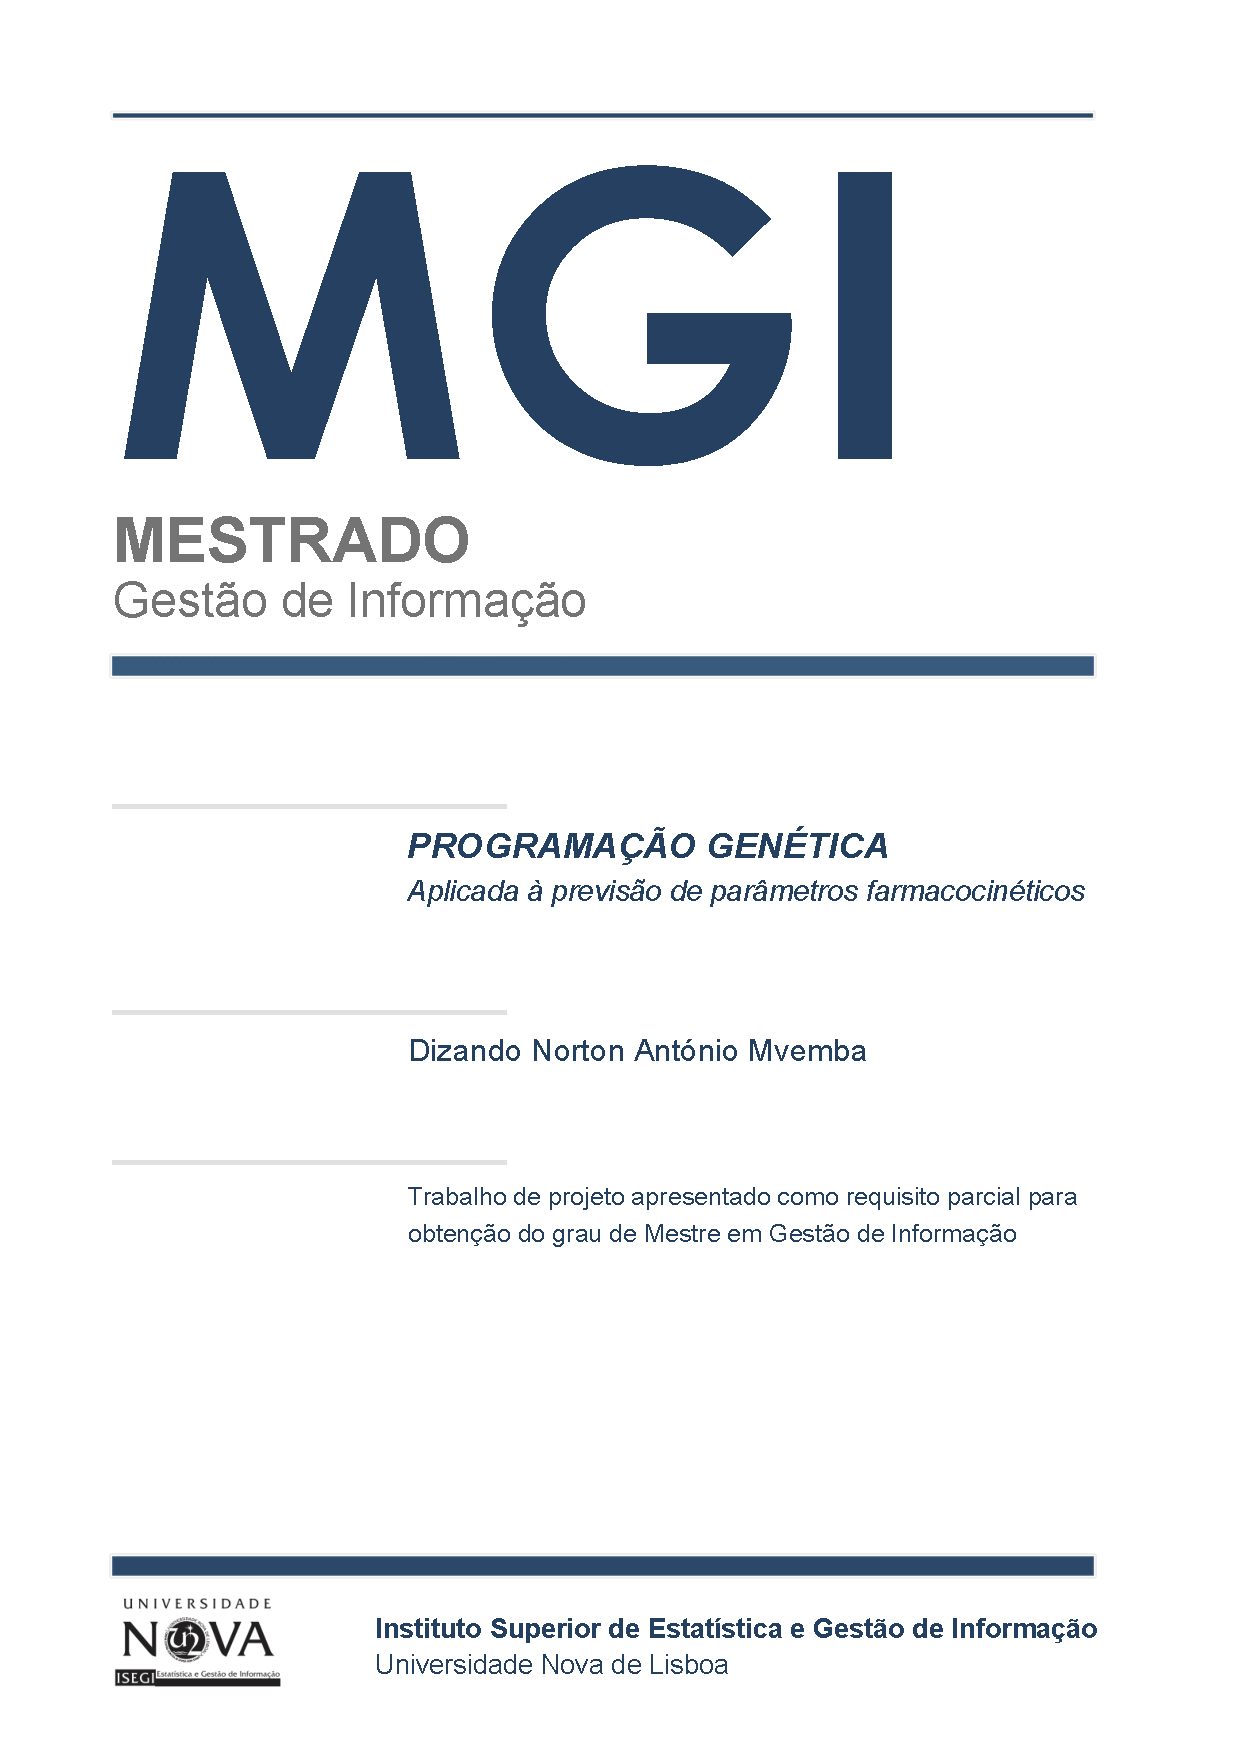
\includepdf[pages=-]{capa.pdf}
%\setcounter{page}{1} \pagenumbering{Alph}

% Add PDF bookmark 
\pdfbookmark[0]{Título}{Título}

\thispagestyle{empty}
%\begin{flushleft} ~\\ \vspace{-10mm} \hspace{-9mm}  %
\includegraphics[width=90mm, height=23mm]{Cover/istlogo} 
%\\ \vspace{5mm}
%~\\ \vspace{50mm} % gr�ficos
%~\\ \begin{center} 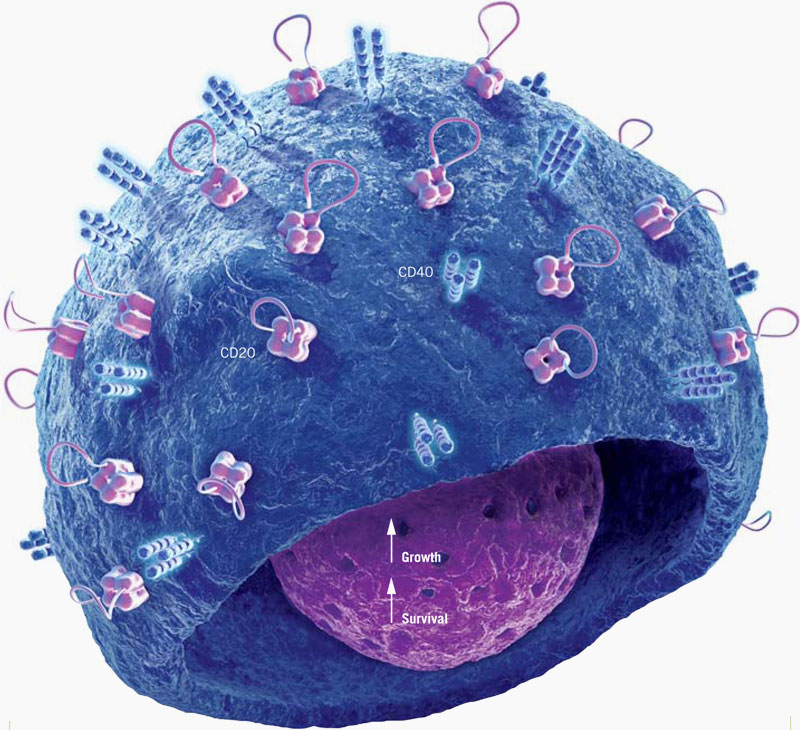
\includegraphics[height=50mm]{Cover/coverimage}  \end{center} % gráficos
~\\ \vspace{5mm}
\begin{centering}
\normalsize Instituto Superior de Estatística e Gestão de Informação\\
\normalsize Universidade Nova de Lisboa
\\ \vspace{30mm}
\large \textbf{PROGRAMAÇÃO GENÉTICA APLICADA A PREVISÃO DE PARÂMETROS FARMACOCINÉTICOS}
\\ \vspace{10mm}
\normalsize por
\\ \vspace{10mm}
\large Dizando Norton António Mvemba (M2012341) % e à previsão do ano de lançamento de músicas
\\ \vspace{30mm}
\setstretch{1.5}
\normalsize Trabalho de projeto apresentado como requisito parcial para a obtenção do grau de Mestre em Gestão de Informação, 
Especialização em Gestão do Conhecimento e Business Intelligence
\\ \vspace{30mm}

\begin{tabular}{c}
\setstretch{1.5}
\normalsize{Orientador: Leonardo Vanneschi, Ph.D} \\
\normalsize{Co-Orientador: Mauro Castelli, Ph.D} \\
\end{tabular}
 
\vspace{25mm}

%\Large \textbf{\todaythesis\today} \\
\normalsize Abril de 2014 \\
\end{centering}
\let\thepage\relax
%\end{flushleft}
\pagebreak


\clearpage
% Since I am using double sided pages, the second page should be white.
% Remember that when delivering the dissertation, IST requires for the cover to appear twice.

\thispagestyle{empty}
\cleardoublepage

\setcounter{page}{1} \pagenumbering{roman}

\baselineskip 18pt % line spacing: -12pt for single spacing
                   %               -18pt for 1 1/2 spacing
                   %               -24pt for double spacingnts} % Uncomment for normal cover with IST logo.
%\setcounter{page}{1} \pagenumbering{Alph}

% Add PDF bookmark 
\pdfbookmark[0]{Title}{Title}

\thispagestyle{empty}
\begin{flushleft} ~\\ \vspace{-10mm} \hspace{-9mm}  
\includegraphics[width=90mm, height=23mm]{Cover/istlogo} \hspace{49mm}  
\includegraphics[height=23mm]{Cover/fml} 
\\ \vspace{5mm}
%~\\ \vspace{50mm} % gr�ficos
~\\ \begin{center} 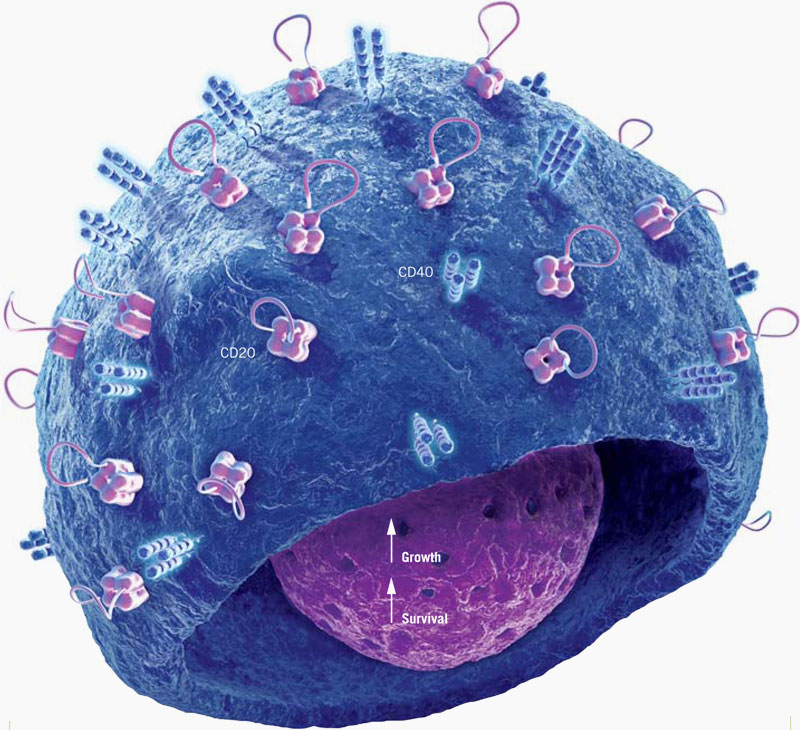
\includegraphics[height=50mm]{Cover/coverimage}  \end{center} % gr�ficos
~\\ \vspace{5mm}
\begin{centering}
\LARGE \textbf{Fancy Title 1}
\\ \vspace{5mm}
\Large Fancy Subtitle 1
\\ \vspace{15mm}
\Large \textbf{Full Name} \\
(Licenciado)
\\ \vspace{15mm}
\Large Dissertação para a obtenção do grau de Mestre em
\\ \vspace{2mm}
\LARGE \textbf{Gestão de Informação}
\\ \vspace{20mm}

\Large \textbf{J�ri}

\begin{tabular}{lcl}
\large Presidente:		&   & \large \\ 
\large Orientador: 		&   & \large \\ 
\large Co-Orientador: &   & \large \\ 
\large Vogal:	 				&   & \large \\
\end{tabular}
 
\vspace{9mm}

%\Large \textbf{\todaythesis\today} \\
\Large \textbf{Janeiro 2012} \\
\end{centering}
\let\thepage\relax
\end{flushleft}
\pagebreak


\clearpage
% Since I am using double sided pages, the second page should be white.
% Remember that when delivering the dissertation, IST requires for the cover to appear twice.

\thispagestyle{empty}
\cleardoublepage

\setcounter{page}{1} \pagenumbering{roman}

\baselineskip 18pt % line spacing: -12pt for single spacing
                   %               -18pt for 1 1/2 spacing
                   %               -24pt for double spacingnts} % Uncomment for Biomedical Engeneering Cover with IST and FMUL logos.
\setcounter{page}{1} \pagenumbering{Alph}

% Add PDF bookmark 
\pdfbookmark[0]{Título}{Título}

\thispagestyle{empty}
%\begin{flushleft} ~\\ \vspace{-10mm} \hspace{-9mm}  %
\includegraphics[width=90mm, height=23mm]{Cover/istlogo} 
%\\ \vspace{5mm}
%~\\ \vspace{50mm} % gr�ficos
%~\\ \begin{center} 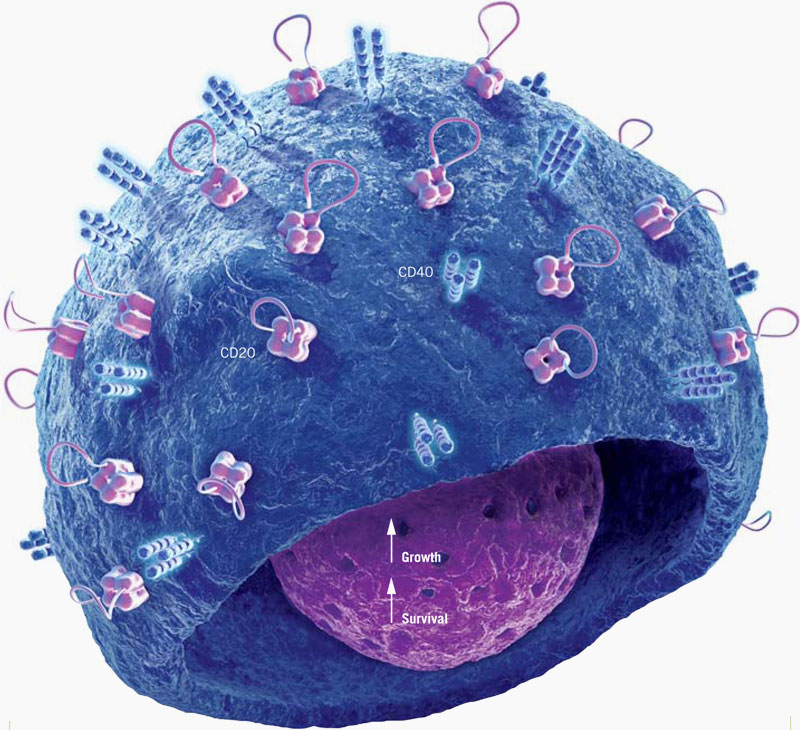
\includegraphics[height=50mm]{Cover/coverimage}  \end{center} % gráficos
~\\ \vspace{5mm}
\begin{centering}
\normalsize Instituto Superior de Estatística e Gestão de Informação\\
\normalsize Universidade Nova de Lisboa
\\ \vspace{30mm}
\large \textbf{PROGRAMAÇÃO GENÉTICA APLICADA A PREVISÃO DE PARÂMETROS FARMACOCINÉTICOS}
\\ \vspace{10mm}
\normalsize por
\\ \vspace{10mm}
\large Dizando Norton António Mvemba (M2012341) % e à previsão do ano de lançamento de músicas
\\ \vspace{30mm}
\setstretch{1.5}
\normalsize Trabalho de projeto apresentado como requisito parcial para a obtenção do grau de Mestre em Gestão de Informação, 
Especialização em Gestão do Conhecimento e Business Intelligence
\\ \vspace{30mm}

\begin{tabular}{c}
\setstretch{1.5}
\normalsize{Orientador: Leonardo Vanneschi, Ph.D} \\
\normalsize{Co-Orientador: Mauro Castelli, Ph.D} \\
\end{tabular}
 
\vspace{25mm}

%\Large \textbf{\todaythesis\today} \\
\normalsize Abril de 2014 \\
\end{centering}
\let\thepage\relax
%\end{flushleft}
\pagebreak


\clearpage
% Since I am using double sided pages, the second page should be white.
% Remember that when delivering the dissertation, IST requires for the cover to appear twice.

\thispagestyle{empty}
\cleardoublepage

\setcounter{page}{1} \pagenumbering{roman}

\baselineskip 18pt % line spacing: -12pt for single spacing
                   %               -18pt for 1 1/2 spacing
                   %               -24pt for double spacingnts}
\thispagestyle{empty}
\hbox{} \vfill
\begin{flushright}
\small \textit{``Essentially, all models are wrong\ldots  but some are useful''}
\\ \vspace{2mm}  
%\scriptsize \emph{Box, George E. P.; Norman R. Draper (1987). Empirical Model-Building and Response Surfaces, p. 424, Wiley. ISBN 0471810339.}
\scriptsize \emph{George E. P. Box}
\end{flushright}

\clearpage
\thispagestyle{empty}
\cleardoublepage
\pdfbookmark{Agradecimentos}{Acknowledgments}
\begin{acknowledgments}
\setstretch{1.5}

Agradeço ao criador Jeová pela vida e pelas bençãos. Toda boa obra, conhecimento e sabedoria que o homem produz é somente porque fomos feitos 
à sua imagem.



Endereço o meu enorme obrigado ao meu orientador e professor, Dr. Leonardo Vanneschi, pelo conhecimento, inspiração e desafios que forneceu
ao longo das aulas e dos encontros para a elaboração do presente trabalho. A forma como transmitiu conhecimentos que pareciam ser complexos
foi fundamental para que eu desse os primeiros passos no tópico que trata este trabalho. Agradeço também ao seu companheiro de trabalho e
meu co-orientador Dr. Mauro Castelli, pela disponibilidade e enorme interesse em ajudar-me quando em dificuldades. Estendo o agradecimento
a Dr. Sara Silva, pelo código-fonte que forneceu e pelas dicas ao utilizar a sua excelente ferramenta de Programação Genética.



Ao meus pais, razão da minha existência, agradeço pelos conselhos e força que me transmitiram mesmo estando distantes. Ao
Bozé Donadoni, por cumprir em pleno o papel de irmão mais velho e amigo, e as minhas irmâs, Kelani e Cristina, pelas conversas sempre
oportunas que me permitiam ``tirar'' a mente do trabalho. À Jeorgina, agradeço por seres meu alicerce e porto seguro. Obrigado pelo amor e pelo suporte, mesmo com as minhas conversas
e explicações intermináveis sobre Programação Genética. Agradeço ao Dr. João Silva, que mostrou-se amigo, e transmitiu-me a coragem necessária para enfrentar este desafio com profissionalismo 
e responsabilidade; espero ter atingido as suas expectativas. Ao Alberto Lourenço, grande amigo, agradeço pela amizade e companheirismo.%; as 
%tuas mensagens muitas vezes encontraram-me em momentos em que precisava delas.



À todas as pessoas que direta ou indiretamente contribuiram para a conclusão do presente trabalho\ldots o meu sincero agradecimento!

\end{acknowledgments}
\clearpage
\thispagestyle{empty}
\cleardoublepage
\begin{resumo}
\setstretch{1.5}
A \ac{PG} é uma técnica de Aprendizagem de Máquina (\ac{ML}) aplicada em problemas de otimização onde pretende-se achar
a melhor solução num conjunto de possíveis soluções. A \ac{PG} faz parte do paradigma conhecido por \ac{CE} que tem como inspiração 
à teoria da evolução natural das espécies para orientar a pesquisa das soluções.

Neste trabalho, é avaliada a performance da \ac{PG} no problema de previsão de parâmetros farmacocinéticos utilizados no processo 
de desenvolvimento de fármacos. Este é um problema de otimização onde, dado um conjunto de descritores moleculares de fármacos e os valores
correspondentes dos parâmetros farmacocinéticos ou de sua atividade molecular, utiliza-se a \ac{PG} para construir uma função matemática 
que estima tais valores. Para tal, foram utilizados dados de fármacos com os valores conhecidos de alguns parâmetros 
farmacocinéticos. Para avaliar o desempenho da \ac{PG} na resolução do problema em questão, foram implementados diferentes modelos de
\ac{PG} com diferentes funções de \emph{fitness} e configurações.

Os resultados obtidos pelos diferentes modelos foram comparados com os resultados atualmente publicados na literatura e os mesmos confirmam que a 
\ac{PG} é uma técnica promissora do ponto de vista da precisão das soluções encontradas, da capacidade de generalização e da correlação 
entre os valores previstos e os valores reais.
\end{resumo}
\begin{palavraschave}
Programação Genética, parâmetros farmacocinéticos, previsão.
\end{palavraschave}
\clearpage
\thispagestyle{empty}
\cleardoublepage
\begin{abstract}
\setstretch{1.5}
\ac{GP} is a \ac{ML} technique used in optimization problems where one tries to find the best solution on
a set of possible solutions. \ac{GP} is part of the \ac{EC} paradigm inspired by the theory of natural
evolution of species to guide the search of solutions.

In this work, we evaluated the performance of \ac{GP} on the problem of prediction of pharmacokinetic parameters used in the drug development 
process. This is an optimization problem where, given a set of drug molecular descriptors and the corresponding values of the pharmacokinetic 
parameters or the molecular activity, \ac{GP} is then used to build a mathematical model that estimates such values. To this end, we used data of drugs 
with known values of some pharmacokinetic parameters. To evaluate \ac{GP} performance in solving the problem at hand, several \ac{GP} models were 
implemented with different fitness functions and configurations.

The results from the different GP models were compared with the results currently published in the literature, and they confirm that \ac{GP} is a 
promising technique from the point of view of the accuracy of the solutions, their generalization ability and the correlation between the 
predicted and the actual values.
\end{abstract}
\begin{keywords}
Genetic programming, pharmacokinetics parameters, prediction.
\end{keywords}
\clearpage
\thispagestyle{empty}
\cleardoublepage
% This is required for the fancy chapters
\renewcommand*{\contentsname}{\hfill \large{ÍNDICE} \hfill}
\dominitoc
\dominilof
\dominilot

%%%%%%%%%%%%%%%%%%%%%%%%%%%%%%%%%%%%%%%%%%%%%%%%%%%%%%%%%%%%%%%%%%%%%%
% List of contents
%\renewcommand{\baselinestretch}{1}
%\pdfbookmark[0]{Índice}{index}
\pdfbookmark[0]{Sumário}{toc}
%\renewcommand{\contentsname}{Sumário}
\setstretch{1.5}
\tableofcontents
% \contentsline{chapter}{References}{\pageref{bib}}
\clearpage
\thispagestyle{empty}
\cleardoublepage
%\renewcommand{\baselinestretch}{1.5}
%%%%%%%%%%%%%%%%%%%%%%%%%%%%%%%%%%%%%%%%%%%%%%%%%%%%%%%%%%%%%%%%%%%%%%

% List of figures
\pdfbookmark[0]{Índice de Figuras}{lof}
%\renewcommand{\listfigurename}{\centerline{\large{ÍNDICE DE FIGURAS}}}
\renewcommand{\listfigurename}{\hfill\bfseries\large ÍNDICE DE FIGURAS}
\listoffigures
\clearpage
\thispagestyle{empty}
\cleardoublepage

%%%%%%%%%%%%%%%%%%%%%%%%%%%%%%%%%%%%%%%%%%%%%%%%%%%%%%%%%%%%%%%%%%%%%%
% List of tables
\pdfbookmark[0]{Índice de Tabelas}{lot}
%\renewcommand{\listtablename}{\large{ÍNDICE DE TABELAS}}
\renewcommand{\listtablename}{\hfill\bfseries\large ÍNDICE DE TABELAS}
\listoftables
\clearpage
\thispagestyle{empty}
\cleardoublepage

% %%%%%%%%%%%%%%%%%%%%%%%%%%%%%%%%%%%%%%%%%%%%%%%%%%%%%%%%%%%%%%%%%%%%%%
% % List of algorithms
% Requires packages algorithmic, algorithm
\pdfbookmark[0]{Índice de Algoritmos}{loa}
\renewcommand{\listalgorithmname}{\hfill\bfseries\large ÍNDICE DE ALGORITMOS\hfill}
\listofalgorithms
\cleardoublepage
\acresetall
% %%%%%%%%%%%%%%%%%%%%%%%%%%%%%%%%%%%%%%%%%%%%%%%%%%%%%%%%%%%%%%%%%%%%%%
 % List of acronyms
\pdfbookmark[0]{Lista de Siglas e Abreviaturas}{loac}

%\chapter*{\large{LISTA DE SIGLAS E ABREVIATURAS}}
\chapter*{\bfseries\large\hfil \hfil LISTA DE SIGLAS E ABREVIATURAS\hfil}
% See more at http://staff.science.uva.nl/~polko/HOWTO/LATEX/acronym.html
\begin{acronym}
\acro{F}[\%F]{Biodisponibilidade Oral}
\acro{PPB}[\%PPB]{\emph{Plasma Protein Binding}}
\acro{ADMET}{Absorção, Distribuição, Metabolismo, Excreção e Toxicidade}
\acro{AE}{Algoritmos Evolutivos}
\acro{AG}{Algoritmo Genético}
\acro{ANN}{\emph{Artificial Neural Networks}}
\acro{CE}{Computação Evolucionária}
\acro{DELOS}{\emph{Discovery and Lead Optimization Systems}}
\acro{EC}{\emph{Evolutionary Computation}}
\acro{EE}{Estratégias de Evolução}
\acro{FDA}{\emph{Food and Drug Administration}}
\acro{GP}{\emph{Genetic Programming}}
\acro{GPLAB}{\emph{Genetic Programming toolbox for MATLAB}}
\acro{HTS}{\emph{High Throughput Screening}}
\acro{LD50}{\emph{Median Lethal Dose}}
\acro{LISP}{\emph{List Processing}}
\acro{LS}{\emph{Linear Scaling}}
\acro{ML}{\emph{Machine Learning}}
\acro{MAPE}{\emph{Mean Absolute Percentage Error}}
\acro{MASE}{\emph{Mean Absolute Scaled Error}}
\acro{MCNS}{\emph{Minimal Criteria Novelty Search}}
\acro{MMFF94}{\emph{Merck Molecular Force Field 94}}
\acro{MOE}{\emph{Molecular Operating Environment}}
\acro{MSE}{\emph{Mean Squared Error}}
\acro{NCI}{\emph{National Cancer Institute}}
\acro{NS}{\emph{Novelty Search}}
\acro{PCC}{Coeficiente de Correlação de \emph{Pearson}}
\acro{PCCN}{Coeficiente de Correlação de \emph{Pearson} Normalizado}
\acro{PE}{Programação Evolutiva}
\acro{PG}{Programação Genética}
\acro{QSAR}{\emph{Quantitative Structure Activity Relationship}}
\acro{R2}[$R^2$]{Coeficiente de determinação}
\acro{RCSBPDB}[RCSB-PDB]{\emph{Research Collabolatory for Structural Bioinformatics - Protein Data Bank}}
\acro{RE}{Robótica Evolutiva}
\acro{RF}{\emph{Random Forests}}
\acro{RMSE}{\emph{Root Mean Squared Error}}
\acro{SMILES}{\emph{Simplified Molecular Input Line Entry Specification}}
\acro{SOM}{\emph{Self Organizing Maps}}
\acro{SVM}{\emph{Support Vector Machines}}
\end{acronym}

\clearpage
\thispagestyle{empty}
\cleardoublepage




%%%%%%%%%%%%%%%%%%%%%%%%%%%%%%%%%%%%%%%%%%%%%%%%%%%%%%%%%%%%%%%%%%%%%%%
% List of symbols
\pdfbookmark[1]{Lista de Símbolos}{los}

\listofsymbols

\clearpage
\thispagestyle{empty}

\cleardoublepage
% Pages number is starting now with arabic style... until now it was on roman mode
\pagenumbering{arabic} \setcounter{page}{1}
\baselineskip 18pt
\pagenumbering{arabic} \setcounter{page}{1}
\baselineskip 18pt
%\pagestyle{document}%Fancy head and foot with lines
\pagestyle{documentsimple}%Simple head
% %%%%%%%%%%%%%%%%%%%%%%%%%%%%%%%%%%%%%%%%%%%%%%%%%%%%%%%%%%%%%%%%%%%%%%
% The Introduction:
% %%%%%%%%%%%%%%%%%%%%%%%%%%%%%%%%%%%%%%%%%%%%%%%%%%%%%%%%%%%%%%%%%%%%%%
\fancychapter{INTRODUÇÃO}
\label{cap:int}

\section{COMPUTAÇÃO EVOLUCIONÁRIA}
\label{sec:computacaoevolucionaria}

A \ac{CE} é um paradigma na área de Inteligência Artificial 
que tem como inspiração a teoria da evolução biológica de Charles Darwin. A teoria de Darwin afirma que a evolução 
dos seres vivos resulta dos processos de seleção, recombinação, reprodução e mutação onde a cada geração apenas sobrevivem os 
indivíduos mais “aptos” da população \citep{Darwin1859}. 

Tradicionalmente a \ac{CE} é composta pelas seguintes áreas ou \ac{AE}:
\begin{itemize}
  	\item {\ac{EE} \citep{Schw75}}
  	\item {\ac{PE} \citep{Fogel1962}} 
	\item {\ac{AG} \citep{Holland1975}}
	\item {\ac{PG} \citep{Koza1992}}
\end{itemize}

Todas estas técnicas partilham do comum objetivo de produzir sistemas automáticos para a resolução de problemas de otimização ou de pesquisa num 
espaço de soluções possíveis. A \tableref{Tabela111} mostra a analogia de alguns dos termos mais utilizados em \ac{CE}.

\begin{table}[H]
    \begin{tabular}{ll}%
    \toprule
    \textbf{Evolução darwiniana} & \textbf{\ac{CE}}\\ 
    \midrule
    Ambiente				& Problema\\ 
    Indivíduo				& Solução candidata\\ 
    Aptidão	(\emph{fitness})	& Qualidade da solução\\
    \bottomrule
    \end{tabular}
    \centering
    \caption{Analogia entre a evolução darwiniana e a \ac{CE}}
    \label{Tabela111}
\end{table}

Os \acp{AG} são o tipo de \ac{AE} mais antigo e mais estudado. Num \ac{AG}, um indivíduo 
é representado por uma cadeia fixa de caracteres. Cada indivíduo representa uma solução para o problema em questão e a sua 
capacidade de resolver tal problema é determinada por uma 
função de aptidão\footnote{Também chamada de função de \emph{fitness}, função-objetivo ou função de custo. Ao longo deste relatório 
será utilizado o termo: função de \emph{fitness}.}.
Ao longo das gerações (ou iterações) do algoritmo, uma nova população é criada contendo os melhores indivíduos da 
geração anterior e outros indivíduos que são produzidos por cruzamento e mutação \citep{mitchell1998introduction}. 
A \figref{Figura111} ilustra o esquema de funcionamento geral de um \ac{AG}.

\begin{figure}[H]
	\centering
	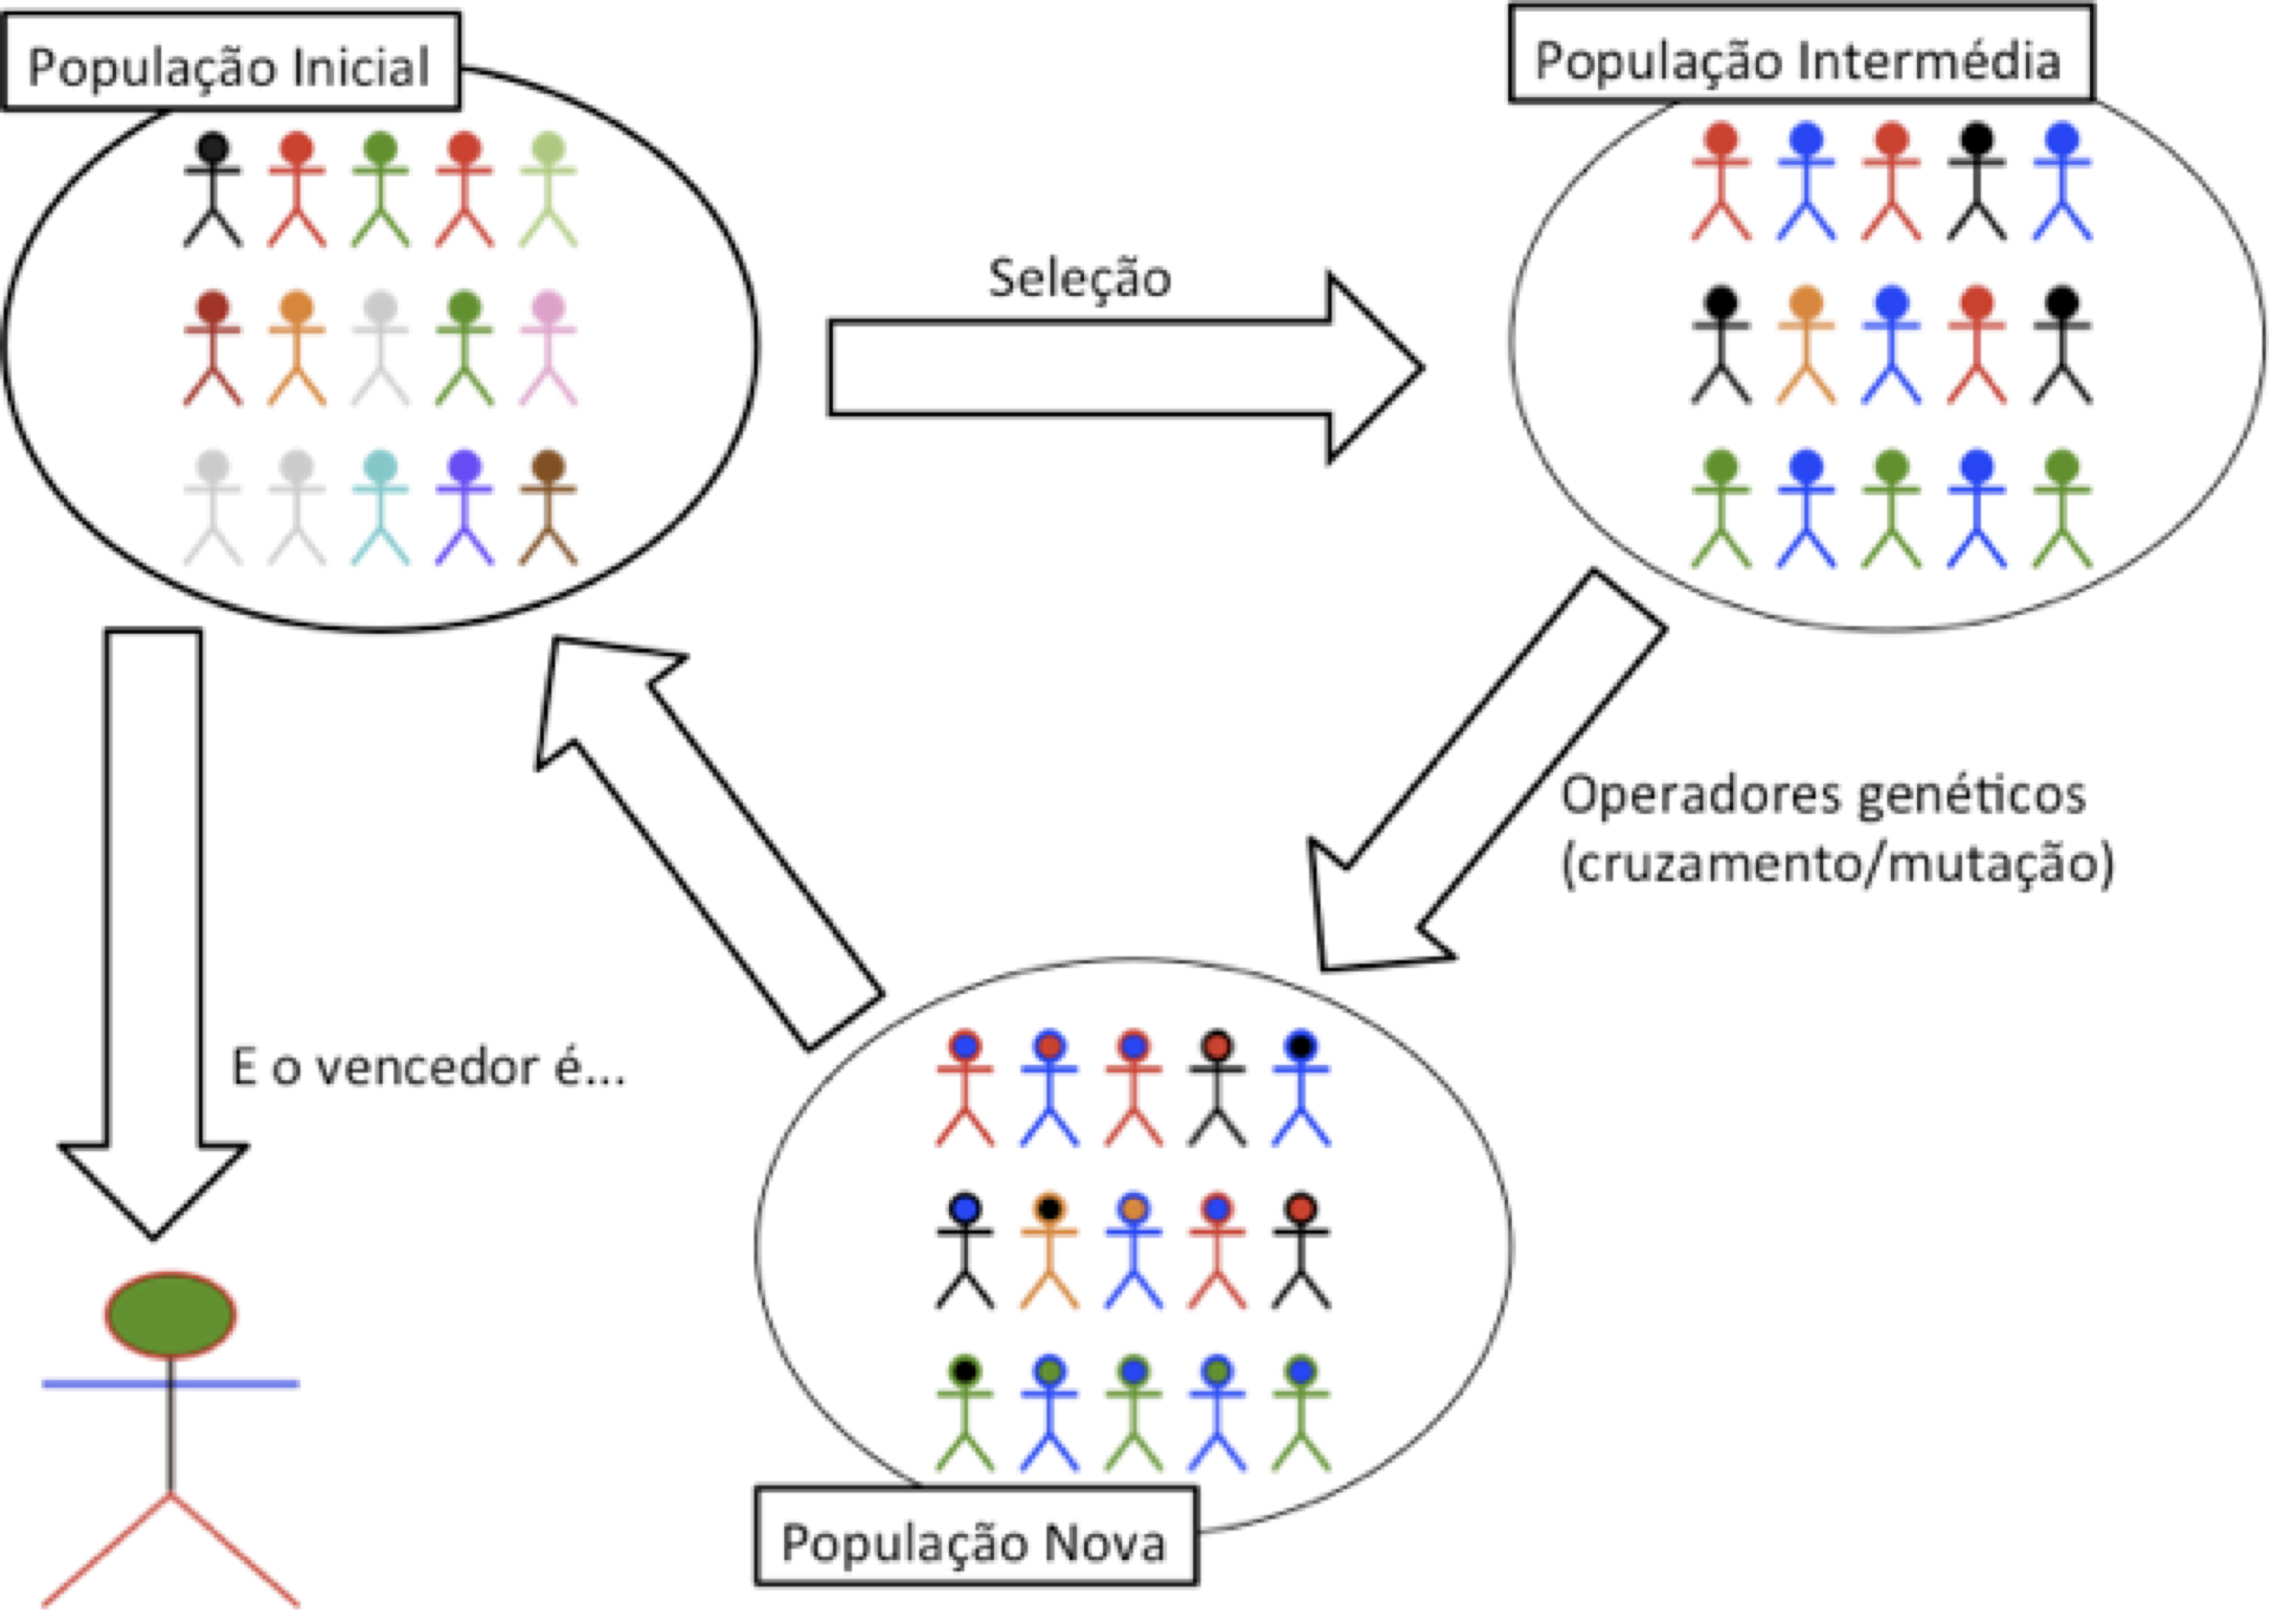
\includegraphics[width=0.75\textwidth]{figures/1}
	\caption{Funcionamento geral de um \ac{AG} padrão}
	\label{Figura111}
\end{figure}

Para a execução de um \ac{AG} deve ser definido à partida o conjunto de caracteres que representam os indivíduos. 
De seguida, é definido também o tamanho $L$ de cada indivíduo, a função de \emph{fitness} e outros parâmetros fundamentais
(e.g. quantidade de indivíduos na população, número máximo de gerações, etc.) \citep{Holland1975}. 
Ao representar os indivíduos com os caracteres binários $0$ e $1$, o tamanho do espaço de pesquisa (ou o conjunto de soluções
possíveis) será $2^L$ ou seja, existirão $2^L$ 
indivíduos diferentes.

O processo, tal como ilustrado na \figref{Figura111}, começa com a criação aleatória de uma população de tamanho $p$. 
Posteriormente o algoritmo entra num ciclo (geração) onde a cada iteração todos os indivíduos são avaliados e recebem um valor de \emph{fitness}. 
Alguns indivíduos são selecionados e copiados para a geração intermédia. Este processo é repetido $p$ vezes para que no final a 
população intermédia tenha exatamente $p$ indivíduos. Alguns indivíduos da população intermediária são escolhidos para reprodução, 
cruzamento ou mutação. O processo termina quando é satisfeito o critério de paragem: um indivíduo da população possui um valor 
de \emph{fitness} satisfatório ou o número máximo de gerações definido a princípio, foi atingido. Os operadores de seleção são utilizados
para escolher os indivíduos que irão fazer parte da reprodução, cruzamento ou mutação. A reprodução é a cópia exata de um indivíduo 
da geração intermediária para a nova geração \citep{Holland1975}. Numa operação de cruzamento dois indivíduos são selecionados e 
combinados gerando dois filhos geralmente diferentes entre si e diferentes dos seus progenitores. Estes novos indivíduos são 
introduzidos na nova população. O método de cruzamento mais conhecido é o \emph{one point crossover} \citep{Holland1975}.
A mutação é uma operação unária, ou seja, requer apenas um indivíduo para a executar. Existem vários métodos de mutação 
mas o mais conhecido é o \emph{point mutation} em que uma posição do indivíduo é escolhida aleatoriamente e o carácter naquela posição 
é substituído por outro carácter escolhido aleatoriamente \citep{Holland1975}.

\subsection{O problema da representação nos Algoritmos Genéticos}

Os \acp{AG} diferenciam-se de uma pesquisa aleatória em parte pelo facto de a cada geração ser gerada nova 
informação para orientar a pesquisa. Apesar da sua simplicidade e utilidade, os \acp{AG} possuem algumas limitações importantes. 
Uma delas, por exemplo, é a impossibilidade de representar soluções hierárquicas, uma vez que as cadeias de caracteres são de 
tamanho fixo. Outra limitação é a impossibilidade de representar estruturas de repetição ou estruturas condicionais que a maior parte dos 
problemas reais exigem \citep{DeJong1985, Koza1992}. Esta habilidade é encontrada nos programas de computador.
\section{INTRODUÇÃO À PROGRAMAÇÃO GENÉTICA}
\label{sec:introgp}

John Koza introduziu o conceito de \ac{PG} onde os indivíduos são representados por programas de computador 
(e.g: expressões matemáticas, expressões lógicas, etc.). Desta forma, em vez de a pesquisa ser feita num conjunto de soluções, 
são gerados programas que automaticamente resolvem o problema sem a necessidade de se saber à partida a estrutura da solução 
\citep{Koza1992}.

Uma forma comum de representar os programas de computador em \ac{PG} é por intermédio de árvores de sintaxe que 
podem ser facilmente transformadas em programas nas linguagens de programação conhecidas. Na implementação
original da \ac{PG}, o \ac{LISP} foi a linguagem de programação utilizada \citep{Koza1992}.

Os indivíduos da população inicial são criados aleatoriamente e ao longo das gerações são produzidos novos indivíduos pela 
aplicação dos operadores genéticos. Os indivíduos mais aptos (com maior valor de \emph{fitness} em problemas de maximização 
ou com menor valor de \emph{fitness} em problemas de minimização) são copiados para as novas gerações ou selecionados para 
cruzamento ou mutação. 

Tal como acontece com os \acp{AG}, as operações de seleção, reprodução, cruzamento e mutação também se aplicam 
ao indivíduos em \ac{PG} (que são programas de computador). Estes e outros aspetos mais avançados sobre a 
\ac{PG} tradicional são o assunto do capítulo \ref{cap:2}.
\section{OBJETIVOS}
\label{sec:objetivos}

Neste trabalho pretende-se aplicar a \ac{PG}
para a previsão de parâmetros farmacocinéticos\footnote{A farmacocinética é o estudo da variação das concentrações plasmáticas dos medicamentos}  
utilizados no desenvolvimento de medicamentos. Posteriormente, será feita uma avaliação da performance da \ac{PG} padrão, comparando-a com a de outras
variantes da \ac{PG}, sobre os mesmos dados.

\subsection{Geral}
Avaliar a \ac{PG} como uma ferramenta computacional bem estabelecida aplicada à resolução de 
problemas reais e de natureza diferente.

\subsection{Específicos}
\begin{itemize}
  \item{Aplicar a \ac{PG} para a previsão de parâmetros farmacocinéticos utilizados no processo de desenvolvimento de medicamentos}
  %\item{Aplicar a regressão simbólica para a previsão do ano de lançamento de músicas}
  \item{Comparar a performance da \ac{PG} padrão com outras variantes de \ac{PG} que utilizam diferentes funções de \emph{fitness}}
  \item{Comparar a \ac{PG} padrão com as outras variantes tendo como critério a complexidade e usabilidade das soluções encontradas}
  \item{Comparar a qualidade dos resultados obtidos pelas diferentes versões de \ac{PG} com os resultados encontrados na literatura sobre os problemas em questão}
\end{itemize}
\section{IMPORTÂNCIA E RELEVÂNCIA}
\label{sec:importancia}

A \ac{PG} tem sido aplicada largamente na resolução de problemas de otimização, (\ac{ML}) e programação automática com 
reconhecido sucesso. A \ac{PG} apresenta muitas vantagens sobre os métodos de otimização convencionais, uma vez que pode lidar
com vários conjuntos de estruturas no espaço de pesquisa, não requerer informação adicional, exceto a definição do objetivo (através 
da função de \emph{fitness}) e pode lidar com problemas que possuem muitos ótimos locais\footnote{Num problema de otimização, um
ótimo local (mínimo ou máximo) é a melhor solução num conjunto vizinho de soluções candidatas. Em contraste, um ótimo global
é a melhor solução entre todas as soluções possíveis, não apenas entre as soluções vizinhas.} e outros \citep{Langdon1996, Banzhaf1998}. 
Desde a sua formalização, experimentos foram realizados em várias áreas com destaque para as seguintes:

\begin{itemize}
\item{Ajustamento de curva e regressão simbólica \citep{Koza1992, Cai2006}}
\item{Processamento de imagens e sinais \citep{Howard20061275}}
\item{Negociação financeira, séries temporais e modelação económica \citep{Chen200575}}
\item{Medicina, Biologia e Bioinformática \citep{Handley1993}}
\item{Jogos de computador e entretenimento \citep{Elyasaf:2011:GES:2001576.2001836}}
\item{Arte \citep{Spector:1994:ccaga}}
\end{itemize}


A pesquisa recente e novas implementações tem feito crescer a aplicabilidade da \ac{PG} em várias 
áreas do saber apresentando resultados comparáveis e muitas vezes melhores que os obtidos por humanos utilizando métodos 
tradicionais ou computacionais. Genericamente a \ac{PG} tem sucesso em problemas complexos, de domínios pouco conhecidos 
e em que não se conhece a estrutura e o tamanho da solução \citep{Poli2008}. Para o presente trabalho, utilizaremos a
regressão simbólica\footnote{A regressão simbólica consiste em induzir (ou descobrir) expressões matemáticas a partir de um conjunto 
dados numéricos multivariados.}, que é a técnica de \ac{PG} mais utilizada em trabalhos empíricos publicados nos últimos anos nas principais
conferências \citep{McDermott:2012:GECCO}.


\subsection{Previsão de parâmetros farmacocinéticos}


O sucesso de um tratamento médico está fortemente correlacionado com a capacidade que uma molécula tem em 
atingir o seu alvo no organismo do paciente sem induzir efeitos tóxicos. 
Além disso, a redução do custo e o tempo relacionado com a descoberta e desenvolvimento de medicamentos é uma 
exigência cada vez mais crucial para a indústria farmacêutica. Portanto, métodos computacionais que permitam 
fazer previsões confiáveis das propriedades dos compostos recém-sintetizados são de extrema relevância \citep{Gunaratna2001}.

Neste trabalho será avaliado o papel da \ac{PG} sobre o problema da previsão de parâmetros farmacocinéticos, 
considerando a estimativa dos processos de \ac{ADMET} a que é 
submetido um medicamento no organismo do paciente.

Será estabelecida uma comparação com outras variantes da \ac{PG} de acordo com a sua capacidade de prever os 
seguintes parâmetros farmacocinéticos: \ac{F}, Dose Oral Letal Mediana (\ac{LD50}) e os níveis de ligação 
às proteínas do plasma (\ac{PPB}). Uma vez que estes parâmetros caracterizam respetivamente a percentagem de dose inicial 
da droga que alcança efetivamente o sistema de circulação sanguínea, os efeitos nocivos e a distribuição do fármaco no organismo, 
eles são essenciais para a seleção de moléculas potencialmente boas \citep{Urso2002}.


%\subsection{Previsão do ano de lançamento de músicas}


%A recuperação de informação musical é uma área multidisciplinar que tem por objetivo obter informação relevante em músicas. 
%Geralmente, as suas técnicas têm aplicações práticas em sistemas de recomendação musical, reconhecimento de instrumentos, 
%transcrição automática de músicas, categorização musical, geração automática de música e outras \citep{Song2012}.

%Os sistemas de recomendação musical formam a área mais largamente estudada em recuperação de informação musical e oferecem 
%sugestões personalizadas de sonoridades, géneros musicais ou artistas similares de acordo com os interesses, o histórico ou o 
%comportamento dos ouvintes. 

%A previsão do ano de lançamento de uma música é uma estimativa feita sobre as características auditivas da música. 
%Ao se prever o ano de lançamento de uma música, um sistema de recomendação pode sugerir aos ouvintes músicas 
%que marcaram certos períodos da sua vida (e.g: a adolescência). Por outra, a criação de um modelo da variação das características 
%auditivas das músicas ao longo dos anos pode ajudar a entender a evolução da música popular. 
%Esta abordagem da previsão do ano de lançamento de músicas através das suas características auditivas é raramente abordada em 
%sistemas de recomendação musical \citep{Bertin-mahieux2011}.

%Neste trabalho pretende-se avaliar a performance da \ac{PG} (regressão simbólica) aplicada ao problema de previsão 
%de ano de lançamento de músicas utilizando dados acústicos de $515.576$ músicas com os respectivos anos de lançamento e compara-la 
%com os resultados publicados até a data da escrita desde relatório em \citep{Bertin-mahieux2011}.
\section{CONTRIBUIÇÃO}
\label{sec:contribuicao}

Para a elaboração das previsões dos parâmetros farmacocinéticos foi utilizado o 
\ac{GPLAB}\footnote{\url{http://gplab.sourceforge.net}} que é uma ferramenta de \ac{PG} para o MATLAB\footnote{O MATLAB 
é um \emph{software} de alta performance dedicado ao cálculo numérico desenvolvido pela MathWorks: \url{www.mathworks.com}}
\citep{Silva2005}. 
Apesar do \ac{GPLAB} ser uma ferramenta robusta e suficiente para a execução de \ac{PG} padrão, ele permite a integração de novas funcionalidades 
(e.g: funções de fitness, operadores genéticos, etc.) na forma \emph{plug-and-play}. Sendo assim, no presente trabalho foram 
acrescentadas as seguintes novas funções \emph{fitness} ao \ac{GPLAB}:

\begin{itemize}
  	\item{\emph{Linear scaling} \citep{keijzer03} (ver secção \ref{LSGP})}
	\item{\ac{MASE} \citep{Hyndman2006} (ver secção \ref{MASEGP})}
	\item{GPBoost \citep{Hyndman2006} (ver secção \ref{BGP})}
\end{itemize}

A pesquisa por novidade (\ac{NS}), tal como definida em \citep{Lehman2008}, é uma técnica utilizada em \ac{RE}, que
simplesmente substitui a função de \emph{fitness} por uma medida de novidade de formas a explorar o espaço de comportamentos
dos indivíduos ao longo das gerações da \ac{PG}. A pesquisa por novidade tem apresentado resultados promissores em vários
experimentos envolvendo \ac{RE}, Neuro Evolução e outras ``novas sub-áreas'' da \ac{CE}, tal como 
descrito em \citep{Lehman2008} e \citep{lehman2010efficiently}.
Para o presente trabalho foi desenvolvida uma nova medida de novidade que implementa o
conceito da pesquisa de novidade para problemas de regressão simbólica (ver secção \ref{NSGP}). Até ao momento, esta é a segunda tentativa para
alcançar tal objetivo, sendo a primeira apresentada em \citep{Trujillo2013}.
\section{ESTRUTURA}
\label{sec:estrutura}

Para além do presente capítulo de introdução, este trabalho de projeto está dividido pelos seguintes outros capítulos:

\begin{itemize}
\item{O capítulo \ref{cap:2} fornece uma introdução a \ac{PG} padrão, %e o seu estado de arte, 
apresentado os principais conceitos}
\item{O capítulo \ref{cap:3} descreve a importância da previsão dos parâmetros farmacocinéticos bem como os principais 
resultados encontrados na literatura}
%\item{Os Sistemas de Recomendação Musical (SRM), suas vantagens e aplicações são brevemente apresentadas no capítulo \ref{cap:4}. No final deste capítulo é apresenta a tarefa de SRM tratada no presente trabalho: previsão do ano de lançamento de músicas.}
\item{O capítulo \ref{cap:5} apresenta a metodologia, técnicas, configurações utilizadas para a recolha e análise dos dados, configuração do ambiente de execução dos testes e a ferramenta utilizada durante o processo de previsão
% (GPLAB). 
%No final do capítulo são apresentadas as extensões feitas ao GPLAB.
}
\item{Os resultados do presente trabalho são apresentados e discutidos no capítulo \ref{cap:6} 
%Posteriormente é elaborada uma comparação com os principais resultados obtidos por outros algoritmos de previsão e com os resultados publicados até ao momento.
}
\item{Finalmente, o capítulo \ref{cap:finais} conclui o presente relatório e traça o caminho para a elaboração de trabalhos futuros
%São também apresentadas as limitações do trabalho.
}
%\item{O código-fonte implementado, as extensões ao GPLAB e outros gráficos são apresentados no Apêndice \ref{ap:a}.}
\end{itemize}

\cleardoublepage
\fancychapter{PROGRAMAÇÃO GENÉTICA}
\label{cap:2}

\section{INTRODUÇÃO}
\label{sec:2introducao}

A \ac{PG} é uma técnica utilizada em \ac{CE} para a resolução de problemas de pesquisa e otimização. 
Em \ac{PG}, diferentemente de uma pesquisa aleatória, o objetivo é fazer com que as soluções melhorem ao longo da execução do
algoritmo através da aplicação de uma função de \emph{fitness}. Durante este processo, os indivíduos mais aptos (ou parte das suas 
características), são preservados através da utilização de operadores genéticos \citep{Koza1992}. No geral, a \ac{PG} cria 
programas de computador para resolver problemas executando os seguintes passos:

\begin{enumerate}
	\item{Cria uma população de programas de computador (soluções, indivíduos).}
  	\item{Executa iterativamente os seguintes passos até que um critério de paragem seja satisfeito:}
  	\begin{enumerate}
    	\item{Executa cada programa na população e atribui um valor de \emph{fitness} de acordo a sua capacidade de resolver
    	o problema.}
    	\item{Cria uma nova população aplicando as seguintes operações:}
    	\begin{enumerate}
    		\item{Seleciona, probabilísticamente, um conjunto de programas de computador para serem reproduzidos com base na
    		sua \emph{fitness} (seleção).}
    		\item{Copia alguns dos programas selecionados, sem modificá-los, para a nova população (reprodução).}
    		\item{Cria novos programas de computador por combinar genéticamente partes de dois indivíduos selecionadas 
    		aleatoriamente (cruzamento).}
    		\item{Cria novos programas de computador por substituir partes selecionadas aleatoriamente de um indivíduo por
    		novos indivíduos criados aleatoriamente (mutação).}
    	\end{enumerate}
  	\end{enumerate}
  	\item{Os melhores programas de computador encontrados numa geração são o resultado do processo de \ac{PG} para tal geração.
  	Este resultado pode ser uma solução (ótima ou aproximada) para o problema.}
\end{enumerate}

Nas próximas secções, cada um destes passos é apresentado em mais detalhes.

\section{REPRESENTAÇÃO DOS INDIVÍDUOS}
\label{sec:2representacao}

Os \acp{AG} diferem da \ac{PG} essencialmente pela forma como os indivíduos são 
representados e codificados. Nos \acp{AG}, os indivíduos são representados por uma cadeia fixa de caracteres 
(geralmente binários), tal como ilustrado na \figref{Figura221}.

%\begin{figure}[H]
%	\centering
%	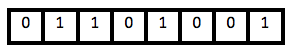
\includegraphics[width=0.5\textwidth]{figures/2}
%	\caption{Representação de um indivíduo em cadeia de caracteres binários}
%	\label{Figura221}
%\end{figure}
\vspace*{1mm}
\begin{figure}[H]
	\centering
	\makebox[\textwidth]{} \par
	\fbox{$0$}\fbox{$1$}\fbox{$1$}\fbox{$0$}\fbox{$1$}\fbox{$0$}\fbox{$0$}\fbox{$1$}
	\caption{Representação de um indivíduo em cadeia de caracteres binários}
	\label{Figura221}
\end{figure}
\vspace*{1mm}

A representação em cadeia fixa de caracteres carece de uma propriedade importante e usualmente encontrada nas soluções de 
problemas complexos: a organização hierárquica das soluções em tarefas e subtarefas \citep{Koza1992}. Para além desta deficiência, 
outras foram levantadas em \citep{DeJong1985} e \citep{Koza1992}.

Na \ac{PG} os indivíduos são programas de computador. Estes indivíduos são geralmente representados em árvores de 
sintaxe, mas existem outras formas de representação como por exemplo: linear \citep{Banzhaf1993,Kinnear:Nordin}, 
em grafo \citep{Poli:1996:nnPDGP,Teller:1996:aigp2} e cartesiana \citep{MS:IEEETEC:06,miller:1999:ACGP}. 
Neste trabalho adoptou-se a representação mais comum: árvores de sintaxe \citep{Koza1992}.

As árvores de sintaxe são construídas a partir de um conjunto de funções \\
$F=\{f_1,\ldots,f_n\}$ que representam os nós da árvore
e um conjunto de símbolos terminais $T=\{t_1,\ldots,t_n\}$ que representam as folhas da árvore. 
Assim, o espaço de procura de soluções é constituído por todas as expressões que podem ser construídas recursivamente com as 
funções em $F$ e os símbolos terminais em $T$. 

Cada função do conjunto $F$ pode ser uma função aritmética, matemática, lógica ou outra, que aceite um determinado número de 
argumentos (aridade) \citep{Koza1992}. Um elemento do conjunto $T$ pode ser uma variável ou uma constante definida sobre o 
domínio do problema. A \figref{Figura222}, apresenta uma árvore válida construída “aleatoriamente” a partir dos conjuntos $F=\{{+,-,*,/}\}$ 
e $T=\{{x_1,x_2}\}$.

\begin{figure}[H]
	\centering
	\begin{tikzpicture}[every node/.style={circle,draw}] 
    	\tikzstyle{level 1}=[sibling distance=2.5cm] 
    	\tikzstyle{level 2}=[sibling distance=1.5cm] 
    	\node {$+$}
	    child{node {$*$} child{node {$x_1$}} child{node {$x_2$}}}
	    child{node {$-$} child{node {$x_1$}} child{node {$x_2$}}};
	\end{tikzpicture}%
	\caption{Exemplo de um indivíduo em \ac{PG}}
	\label{Figura222}
\end{figure}

Esta árvore corresponde a expressão matemática,

\begin{equation}
f(x_1,x_2) = (x_1*x_2) + (x_1-x_2)
\label{Equacao221}
\end{equation}

As funções em $F$ devem obedecer a propriedade do fechamento para garantir consistência nos tipos de dados e segurança na avaliação 
das expressões por elas criadas \citep{Poli2008}. Considerando a expressão da \equationref{Equacao221} que representa o 
indivíduo da \figref{Figura222}, a consistência 
nos tipos de dados consiste em garantir que os valores para as variáveis $x_1$ e $x_2$ estejam definidos para os operadores de 
adição ($+$) e subtração ($-$). Mesmo respeitando esta propriedade algumas funções podem falhar ao serem executadas. 
Um caso comum, é a divisão por $0$. Koza introduziu uma nova operação, a divisão protegida (${\%}$), que retorna o valor $1$ sempre que 
o denominador for igual a $0$ \citep{Koza1992}.

Os elementos dos conjuntos $F$ e $T$ devem ser suficientes para representar as soluções do problema dado. Esta propriedade de 
suficiência, nem sempre é satisfeita porque antes da execução do algoritmo a estrutura da solução não é conhecida, e logo, não há 
garantia que os elementos em $F$ e $T$ sejam suficientes para representar a solução do problema. Um exemplo de um conjunto suficiente é o conjunto $F =\{{AND,OR,NOT}\}$ que só 
por si é adequado para representar qualquer função \emph{booleana} \citep{Koza1992}.
\section{INICIALIZAÇÃO DA POPULAÇÃO}
\label{sec:2inicializacao}

Os indivíduos na população inicial são criados aleatoriamente tal como nos \acp{AG} porém, os métodos utilizados para tal 
são diferentes. Em \ac{PG} existem três métodos comuns de inicialização:

\begin{itemize}
\item{Método completo (\emph{full})}
\item{Método de crescimento (\emph{grow})}
\item{Método em rampa meio-a-meio (\emph{ramped half-and-half})} 
\end{itemize}

No método completo, uma função é selecionada aleatoriamente do conjunto de funções $F$ para ser o nó raiz. De seguida, outras funções são selecionadas 
também aleatoriamente em $F$ para formar os outros nós da árvore. A profundidade\footnote{A profundidade de uma árvore é a quantidade de nós que devem ser percorridos
desde a raiz da árvore até ao nó mais profundo (folha).} máxima da árvore é preenchida apenas por símbolos terminais selecionados 
aleatoriamente no conjunto de terminais $T$. Dessa forma, são criadas árvores completas em que todas as folhas se encontram à mesma 
profundidade. O \algreff{Algoritmo231} contém o pseudocódigo para o método \emph{completo}.

\begin{algorithm}[H]
	\caption{Método de Inicialização Completo}
	\label{Algoritmo231}
	\begin{algorithmic}[1]
		\Function{completo}{$profMaxima$}
			\If {$profMaxima = 1$}
				\State {$no \gets n \in \mathbb{N}, \Call{aridade}{n} = 0$}
			\Else
				\State {$no \gets n \in \mathbb{N}, \Call{aridade}{n} \neq 0$}
				\For {$i \gets 1:\Call{aridade}{n}$}%
					\State {$\Call{addDescendente}{no, \Call{completo}{profMaxima - 1}}$}%
				\EndFor
			\EndIf
			\State \Return {$no$}
		\EndFunction
	\end{algorithmic}
\end{algorithm}

No \algreff{Algoritmo231}, $profMaxima$ é a profundidade máxima da árvore, $\mathbb{N}$ é o conjunto formado pelas funções
em $F$ e os símbolos em $T$, e $n$ é um elemento de $\mathbb{N}$. A função $\Call{aridade}{n}$ determina o número de argumentos
ou operandos de $n$. Quando a aridade de $n$ é igual a zero ($\Call{aridade}{n} = 0$), isto significa que $n$ é um símbolo
terminal. A função $\Call{addDescendente}{no, \Call{completo}{profMaxima-1}}$ conecta o nó-filho $no$ ao seu nó-pai e acrescenta
os outros nós à árvore de forma recursiva.

O método de \emph{crescimento} funciona de forma quase semelhante ao método \emph{completo}, exceto que não são criadas árvores completas 
ou cheias, pois os nós são selecionados aleatoriamente de um conjunto formado pelas funções e os símbolos terminais. Sempre que 
for selecionado um símbolo terminal, o crescimento da árvore para aquele nó termina mesmo que não tenha sido atingida a profundidade 
máxima. O \algreff{Algoritmo232} ilustra o pseudocódigo para o método de \emph{crescimento}.

\begin{algorithm}[H]
	\caption{Método de Inicialização de Crescimento}
	\label{Algoritmo232}
	\begin{algorithmic}[1]
		\Function{crescimento}{$profMaxima$}
			\If {$profMaxima = 1$}
				\State {$no \gets n \in \mathbb{N}, \Call{aridade}{n} = 0$}
			\Else
				\State {$no \gets n \in \mathbb{N}$}
				\For {$i \gets 1:\Call{aridade}{n}$}%
					\State {$\Call{addDescendente}{no, \Call{crescimento}{profMaxima - 1}}$}%
				\EndFor
			\EndIf
			\State \Return {$no$}
		\EndFunction
	\end{algorithmic}
\end{algorithm}

O método \emph{completo} assume a princípio uma estrutura completa para os indivíduos e o método de \emph{crescimento} pode gerar árvores muito 
curtas, caso existam muitos elementos de aridade igual a $0$ (símbolos terminais) \citep{Poli2008}. Numa inicialização em 
\emph{rampa meio-a-meio}, metade da população é criada com o método \emph{completo} e a outra metade é criada com o método de 
\emph{crescimento}. Este procedimento permite a construção de árvores de tamanhos e configurações diferentes, garantindo assim 
a diversidade na população \citep{Koza1992}. O pseudocódigo para o método em \emph{rampa meio-a-meio} é apresentado no \algreff{Algoritmo233}.

\begin{algorithm}[H]
	\caption{Método de Inicialização em Rampa Meio-a-Meio}
	\label{Algoritmo233}
	\begin{algorithmic}[1]
		\Function{rampa}{$profMaxima, probCrescimento$}
			\State {$profundidade \gets \Call{aleatorio}{1,profMaxima}$}%
			\If {$\Call{aleatorio}{0,1} < probCrescimento$}%
				\State \Return {$\Call{crescimento}{profundidade}$}
			\Else
				\State \Return {$\Call{completo}{profundidade}$}
			\EndIf
		\EndFunction
	\end{algorithmic}
\end{algorithm}

No \algreff{Algoritmo233}, $probCrescimento$ é um parâmetro que determina a probabilidade de selecionar o método 
\emph{completo} ou o método
de \emph{crescimento} ao construir uma árvore. A variável $profundidade$ recebe um valor aleatório, entre
$1$ e $profMaxima$, que determina o tamanho para a árvore a ser construída.
\section{FUNÇÃO DE \emph{FITNESS}}
\label{sec:2funcaofitness}

A capacidade que um indivíduo tem em resolver um problema é quantificada pela função de \emph{fitness}. 
A função de \emph{fitness} avalia a performance do indivíduo executando-o num conjunto de casos de aptidão conhecidos. 
Num problema de regressão simbólica, em que se pretende ajustar uma expressão à um conjunto de dados, os casos de aptidão 
(ou casos de \emph{fitness}) são os valores que as variáveis independentes\footnote{Também conhecida
por: variável de entrada, característica, variável de previsão, atributo, etc.} assumem nos diferentes pontos desse conjunto.

\subsection{\emph{Fitness} bruto}
\label{subsec:2fitnessbruto}

Considerando o valores para $x_1$ e $x_2$ (variáveis independentes) e $y$ (variável dependente\footnote{Também conhecida
por: variável de saída, variável de resposta, valor de saída, etc.}) representados na \tableref{Tabela241}, o trabalho 
da regressão simbólica consistirá em encontrar uma função $f(x_1,x_2)$ que produz valores de saída iguais ou aproximados aos de $y$. 
Uma possível solução é o indivíduo representado pela \figref{Figura222} que origina a função $f(x_1,x_2)= (x_1*x_2 )+(x_1-x_2)$.

\begin{table}[H]
    \begin{tabular}{rrr}%
    \toprule
   	$x_1$ 	&	$x_2$	&	$y$\\ 
   	\midrule
    $1$		&	$-1$	&	$0$\\ 
    $0$		&	$1$		&	$-1$\\ 
   	$-2$	&	$2$		&	$15$\\ 
    $-1$	&	$2$		&	$-8$\\ 
    $2$		&	$-1$	&	$7$\\
    \bottomrule %
    \end{tabular} %
    \centering
    \caption{Casos de \emph{fitness}}
    \label{Tabela241}
\end{table}

Para avaliar a capacidade da função $f(x_1,x_2)$ se ajustar aos dados da \tableref{Tabela241}, deve-se tradicionalmente calcular uma 
medida de erro. Uma medida de erro muito utilizada é o erro quadrático médio (\ac{MSE}), dado pela fórmula:

\begin{equation}
\emph{MSE} = \frac{1}{n}\sum_{i=1}^{n} (y_i-f_i)^2
\label{Equacao241}
\end{equation}
\noindent onde $n$ é o número de casos de \emph{fitness} (linhas, registos ou exemplos), $y_i$ são os valores de saída conhecidos e $f_i$ são os valores 
gerados por \equationref{Equacao221}. Ao aplicar a \equationref{Equacao221} e a \equationref{Equacao241} ao nosso exemplo, obtêm-se os resultados na \tableref{Tabela242}.

\begin{table}[H]
    \begin{tabular}{rrrrr}%
    \toprule
    $x_1$ 	&	$x_2$	&	$y$		&	$f(x_1,x_2)$	& 	$(y-f)^2$\\
    \midrule
    $1$		&	$-1$	&	$0$		&	$1$				&	$1$\\ 
    $0$		&	$1$		&	$-1$	&	$-1$			&	$0$\\ 
   	$-2$	&	$2$		&	$15$	&	$-8$			&	$49$\\ 
    $-1$	&	$2$		&	$-8$	&	$-5$			&	$9$\\ 
    $2$		&	$-1$	&	$7$		&	$1$				&	$36$\\
    		&			&	~		&	\textbf{\emph{MSE}}	&	$95$\\  
    \bottomrule %
    \end{tabular} %
    \centering
    \caption{Valores para $y$, $f$ e erro quadrático médio de $f$}
    \label{Tabela242}
\end{table}

O valor obtido ($95$), é o \emph{fitness} bruto do indivíduo representado pela \figref{Figura222},  para os casos de aptidão na \tableref{Tabela241}. 
O \emph{fitness} bruto expressa a aptidão da solução numa terminologia natural do problema \citep{Koza1992}.

\subsection{\emph{Fitness} padronizado}

O \emph{fitness} padronizado é uma transformação ao \emph{fitness} bruto de formas a que um valor menor de \emph{fitness}, é considerado melhor.
Em muitos casos é conveniente e desejável fazer com que o melhor valor de \emph{fitness} padronizado seja igual a zero. Isto pode ser obtido através da
soma ou subtração de uma constante. Num problema em que um valor de \emph{fitness} bruto é melhor e o valor máximo de \emph{fitness} bruto é conhecido,
o \emph{fitness} padronizado pode ser obtido pela fórmula:

\begin{equation}
f_S(i)=f^{max}_R - f_R(i)
\label{Equacao242}
\end{equation}
\noindent onde $f_R(i)$ é o \emph{fitness} bruto de $i$.
\section{SELEÇÃO}
\label{sec:2selecao}

Após a determinação da aptidão dos indivíduos da população numa geração, deve-se decidir se os indivíduos serão copiados ou selecionados para 
cruzamento ou mutação. Esta é a função dos operadores de seleção. Existem vários operadores de seleção mas, os mais utilizados são:
a seleção proporcional à \emph{fitness} (roleta russa), a seleção por classificação (\emph{ranking}) e a seleção por torneio.

Na seleção proporcional à \emph{fitness} um indivíduo é selecionado com base numa probabilidade que é dada por:
\begin{equation}
p_i = \frac{f_i}{\sum{f}}
\label{Equacao251}
\end{equation}
\noindent onde $p_i$ é a probabilidade de o indivíduo $i$ ser selecionado e $f_i$ é a \emph{fitness} de $i$.

Na seleção por classificação os indivíduos são ordenados com base no seu \emph{fitness}. De seguida é designada uma probabilidade a cada indivíduo em 
função da sua ordem na população. Normalmente são utilizadas classificações lineares e exponenciais.

A seleção por torneio, diferentemente das outras duas apresentadas anteriormente, não é baseada numa “competição” entre todos os indivíduos da 
população. Apenas um número de indivíduos (chamado tamanho do torneio) é selecionado aleatoriamente. O indivíduo com o melhor \emph{fitness} nesse 
grupo é escolhido. Este procedimento é repetido $N$ vezes, onde $N$ é o tamanho da população.  Este método é amplamente utilizado em \ac{PG} 
principalmente porque não requer uma comparação de \emph{fitness} centralizada entre todos os indivíduos. Este método também permite poupar o processamento computacional.
\section{CRUZAMENTO}
\label{sec:2cruzamento}

O operador de cruzamento (recombinação sexual) introduz diversidade na população por produzir novos indivíduos (filhos) que são compostos por partes 
retiradas de cada um dos pais. Os pais são escolhidos através dos métodos de seleção apresentados na secção \ref{sec:2selecao}.
O método mais comum de cruzamento é o cruzamento de subárvore \citep{Koza1992} que funciona da seguinte forma:

\begin{itemize}
  \item {Seleciona dois indivíduos (pais) utilizando um método de seleção}
  \item {Seleciona uma subárvore aleatória em cada um dos pais. A raíz dessa subárvore é o nó ou ponto de cruzamento\footnote{É 
  comum, e conveniente, que subárvores constituídas por símbolos terminais ou pelo nó-raiz sejam selecionadas
  com probabilidade baixa em relação as outras pois esta é provavelmente uma das causas do fenómeno conhecido por \emph{bloat},
  que é o crescimento excessivo das árvores sem uma correspondente melhoria da \emph{fitness}.}}
  \item {Cria dois novos indivíduos (filhos) por trocar as duas subárvores selecionadas entre os pais.}
\end{itemize}

A \figref{Figura261} ilustra um exemplo de um cruzamento de subárvore.

%\begin{figure}[H]
%	\centering
%	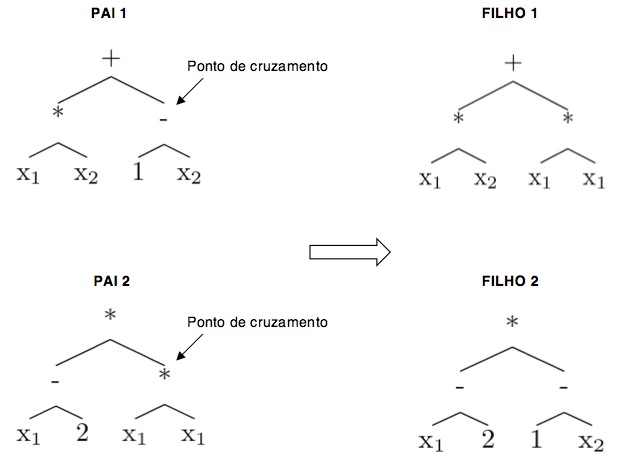
\includegraphics[width=0.75\textwidth]{figures/3}
%	\caption{Exemplo de um cruzamento de subárvore}
%	\label{Figura261}
%\end{figure}

\begin{figure}[H]
	\centering
	\begin{forest}
		for tree={child anchor=north}
		[, phantom, s sep = 2.5cm,
			%for tree={circle, draw}
			[{Pai 1}, name=pai1, baseline, for children={no edge}
				[$+$,circle,draw,
					[$*$,circle,draw
						[$x_1$,circle,draw]
						[$x_2$,circle,draw]
					]
					[,phantom]
					[$-$,name=p1p,circle,draw,fill=gray,tikz={\node [draw,red,fit to tree,dashed] {};}
						[$1$,circle,draw,name=cima]
						[$x_2$,circle,draw]
					]
				]
			]
			[{Pai 2}, name=pai2, baseline, for children={no edge}, below = 5.5cm
				[$*$,circle,draw,
					[$-$,circle,draw
						[$x_1$,circle,draw]
						[$2$,circle,draw]
					]
					[,phantom]
					[$*$,circle,draw, name=p2p,fill=gray,tikz={\node [draw,red,fit to tree,dashed] {};}
						[$x_1$,circle,draw,name=baixo]
						[$x_1$,circle,draw]
					]
				]
			]
			[{Filho 1}, name=filho1, baseline, for children={no edge}
				[$+$,circle,draw,
					[$*$,circle,draw
						[$x_1$,circle,draw]
						[$x_2$,circle,draw]
					]
					[,phantom]
					[$*$,circle,draw,name=f1p, tikz={\node [draw,red,fit to tree,dashed] {};}
						[$x_1$,circle,draw]
						[$x_1$,circle,draw]
					]
				]
			]
			[{Filho 2}, name=filho2, baseline, for children={no edge}, below = 5.5cm
				[$*$,circle,draw,
					[$-$,circle,draw
						[$x_1$,circle,draw]
						[$2$,circle,draw]
					]
					[,phantom]
					[$-$,circle,draw,name=f2p,tikz={\node [draw,red,fit to tree,dashed] {};}
						[$1$,circle,draw]
						[$x_2$,circle,draw]
					]
				]
			]	
		]
		\draw[arrows={-triangle 45},dashed,color=red] (p1p) to [out=south east,in=north east] (f2p);
		\draw[arrows={-triangle 45},dashed,color=red] (p2p) to [out=north east,in=south west] (f1p);
	\end{forest}
	\caption{Exemplo de cruzamento de subárvore. O nó cinzento é o ponto de cruzamento}
	\label{Figura261}
\end{figure}




\section{MUTAÇÃO}
\label{sec:2mutacao}

Outro operador que altera a estrutura de um indivíduo é a mutação. Em \ac{PG} o método mais comum de mutação é a mutação de subárvore que
seleciona aleatóriamente um ponto (nó) numa árvore e substitui a subárvore com raíz nesse ponto por uma outra subárvore gerada aleatóriamente.
A \figref{Figura271} ilustra um exemplo de um mutação de subárvore.

\begin{figure}[H]
	\centering
	\begin{forest}
		[, phantom, s sep = 2.5cm,
			[{Pai}, baseline, for children={no edge}
				[$+$,circle,draw,
					[$*$,circle,draw
						[$x_1$,circle,draw]
						[$2$,circle,draw]
					]
					[,phantom]
					[$-$,circle,draw
						[$x_1$,circle,draw]
						[$x_2$,circle,draw,fill=gray]
					]
				]
			]
			[{Subárvore gerada aleatoriamente}, baseline, for children={no edge}, below = 5.5cm
				[$+$,name=subarvore,circle,draw,tikz={\node [draw,red,fit to tree,dashed] {};}
					[$/$,circle,draw
						[$x_1$,circle,draw]
						[$x_2$,circle,draw]
					]
					[,phantom]
					[$4$,circle,draw
						[$x_1$,circle,draw]
						[$x_2$,circle,draw]
					]
				]
			]
			[{Filho}, baseline, for children={no edge}, below = 2.25cm
				[$+$,circle,draw,
					[$*$,circle,draw
						[$x_1$,circle,draw]
						[$2$,circle,draw]
					]
					[,phantom]
					[$*$,circle,draw
						[$x_1$,circle,draw]
						[$+$,circle,name=fpm,draw
							[$/$,circle,draw
								[$x_1$,circle,draw]
								[$x_2$,circle,draw]
							]
							[,phantom]
							[$4$,circle,draw
								[$x_1$,circle,draw]
								[$x_2$,circle,draw]
							]
						]
					]
				]
			]
		]
		\draw[arrows={-triangle 45},dashed,color=red] (subarvore) to [out=south east,in=south west] (fpm);
	\end{forest}
	\caption{Exemplo de mutação de subárvore. O nó cinzento é o ponto de mutação e é substituído pela subárvore gerada aleatoriamente}
	\label{Figura271}
\end{figure}

Outros operadores de mutação também muito utilizados em \ac{PG} são: mutação de troca e mutação de ponto. A mutação por troca seleciona
aleatoriamente duas subárvores e as troca. A mutação de ponto seleciona aleatóriamente um nó e o susbtitui com um nó aleatório de mesma aridade.
\section{REPRODUÇÃO}
\label{sec:2reproducao}

A reprodução consiste simplesmente em copiar um indivíduo de uma geração para outra sem alterá-lo. Esta operação é geralmente associada a 
uma técnica de \emph{elitismo}. O elitismo garante que um ou mais indivíduos são copiados, inalterados, de uma geração para a outra. 
A proporção $\frac{N}{M}$ entre o tamanho da elite $N$ e o tamanho da população $M$, é chamada de \emph{fracão da elite}.
\section{PARÂMETROS}
\label{sec:2parametros}

Antes de executar a \ac{PG}, é necessário executar os seguintes passos preparatórios:

\begin{itemize}
  \item {Definir o conjunto de terminais $T$}
  \item {Definir o conjunto de funções $F$}
  \item {Escolher a função de \emph{fitness}}
  \item {Definir os parâmetros para controlar execução}
  \item {Escolher o critério de paragem}
\end{itemize}

Por outro lado, os parâmetros para controlar a execução da \ac{PG} são os seguintes:

\begin{itemize}
  \item {Tamanho da população}
  \item {Técnica utilizada para a inicialização da população}
  \item {Algoritmo de seleção}
  \item {Método e taxa de cruzamento}
  \item {Método e taxa de mutação}
  \item {Profundidade máxima das árvores}
\end{itemize}

O critério de paragem é o método que determina o resultado (fim) da execução. A execução pode ser terminada quando for atingido o número máximo de 
gerações ou quando é encontrado um indivíduo com uma \emph{fitness} considerada aceitável. A escolha destes parâmetros é um passo muito importante 
uma vez que os mesmos determinam a performance da \ac{PG}. A definição dos parâmetros escolhidos para o presente trabalho são apresentados no 
capítulo \ref{cap:5}.
%\section{PROBLEMAS DE REFERÊNCIA EM PROGRAMAÇÃO GENÉTICA}
\label{sec:2benchmarks}

Para além do problema de regressão simbólica descrito nas secções anteriores, são regularmente utilizados em experimentos de \ac{PG} os 
seguintes problemas de referência: o multiplexador, paridade e formiga artificial no trilho de Santa Fé \citep{Koza1992}. No entanto, ao longo
dos anos surgiram novas propostas de problemas de referência que preservem a simplicidade de execução dos problemas anteriores e que ao mesmo
tempo tenham as características encontradas nos problemas reais \citep{McDermott:2012:GECCO}. As próximas secções debruçam-se brevemente
sobre alguns dos problemas de referência em \ac{PG}.

\subsection{Multiplexador} 
\subsection{Paridade}
\subsection{Formiga artificial no trilho de Santa Fé}
\subsection{Melhores problemas de referência}
%\section{Problemas em aberto em Programação Genética}
\label{sec:2problemas}

\subsection{Correlação \emph{Fitness} - Distância}
\subsection{Funções sintéticas}
\subsection{Diversidade e convergência prematura}
\subsection{\emph{Bloat} e os métodos para combatê-la}
%\section{Exemplo de execução}
\label{sec:2exemplo}

Esta secção apresenta um exemplo muito simples de execução de regressão simbólica. O problema consiste em encontrar uma função
que se ajuste a um determinado conjunto de dados.

Começamos por definir a função de \emph{fitness} como sendo simplesmente\ldots

Para tal, utilizaremos o seguinte conjunto de parâmetros:\ldots

O processo inicia com a criação da população inicial. Considere como população inicial os seguintes indivíduos:
\begin{enumerate}
  \item {\ldots}
\end{enumerate}

\cleardoublepage
\fancychapter{PARÂMETROS FARMACOCINÉTICOS}
\label{cap:3}

\section{INTRODUÇÃO}
\label{sec:3introducao}

Os medicamentos\footnote{No presente trabalho, os termos \emph{medicamento}, \emph{fármaco} e \emph{droga} serão utilizados alternadamente.} 
receitados para lidar com certas doenças podem por vezes produzir efeitos colaterais sobre o corpo humano\footnote{Por questões 
de simplicidade aqui nos referimos ao corpo humano. No entanto esses conceitos podem ser generalizados à outros animais.}. 
Esses efeitos ou reações adversas podem acontecer nalgum ponto crítico do ciclo de vida do medicamento. Sendo assim, é importante
perceber quais propriedades químicas dos medicamentos produzem o efeito desejado. Este objetivo é alcançado pelo processo de triagem de 
alta produtividade (\ac{HTS}), que é um método computacional para a busca de moléculas relevantes
em enormes quantidades de substâncias que compôem os medicamentos \citep{TDI2013}.

Os resultados obtidos pela triagem de alta produtividade são posteriormente utilizados para otimizar as propriedades de certas moléculas
no processo de fabricação de medicamentos. Além disso, é necessário garantir que os fármacos percorram o caminho apropriado no corpo humano
sem alterar a saúde do paciente. Por esta razão, o comportamento das moléculas é avaliado durante os processos de absorção, distribuição, 
metabolismo e excreção do medicamento no organismo. O estudo deste processo recebe o nome de farmacocinética \citep{DiPiro2010}. 

Em suma, a farmacocinética dá uma resposta a pergunta sobre como o corpo lida com o fármaco e é composta pelas seguintes fases:
\begin{itemize}
  \item {\textbf{Absorção} - é o processso de entrada das substâncias na circulação sanguínea}
  \item {\textbf{Distribuição} - é a dispersão ou disseminaçao das substâncias através dos fluídos e tecidos do corpo}
  \item {\textbf{Metabolismo} - é o reconhecimento, pelo organismo, de que uma substância está presente e a transformação irreversível dos compontes desta
  substância em metabolitos}
  \item {\textbf{Excreção} - é a remoção das substãncias do corpo. Raramente alguns medicamentos acumulam-se nos tecidos do corpo}
  \item {\textbf{Toxicidade} - representa o quanto uma substância pode prejudicar o organismo}
\end{itemize}

Quase metade das falhas no desenvolvimento de compostos fármacológicos são relacionadas com a farmacocinética e a toxicidade dos fármacos,
segundo estudos publicados nos anos de 1991 \citep{Kennedy1997} e 2000 \citep{Kola2004}, tal como ilustrado na \figref{Figura311}.

\begin{figure}[H]
	\centering
	\begin{tikzpicture}[scale = 0.75]
		%\pie[color={blue,cyan,}]{10/, 30/, 0/, 39/, 5/, 11/, 0/, 5/}
		\pie[color={violet!70, cyan, orange, red!70, blue!70, brown!40}]
		{10/, 30/, 39/, 5/, 11/, 5/}
		\pie[pos={7,0}, text=legend, color={violet!70, cyan, yellow, orange, red!70, blue!70, gray, brown!40}]
		{12/Clínicas, 26/Eficâcia, 4/Elaboração, 7/Farmacocinética, 19/Comerciais, 19/Toxicológicos, 7/Custo dos produtos, 6/Outros}
	\end{tikzpicture}
	\caption{Razões para falhas no desenvolvimento de fármacos (valores aproximados). O gráfico da direita ilustra os resultados de 2009
	e o da esquerda os resultados de 2000}
	\label{Figura311}
\end{figure}

Alguns parâmetros farmacocinéticos diretamente correlacionados com o processo \ac{ADMET} serão utilizados neste trabalho, nomeadamente:
a Biodisponiblidade Oral \ac{F}, o nível de Ligação às Proteínas do Plasma (\ac{PPB}) e a Dose Letal Mediana \ac{LD50}\footnote{Para uma lista mais 
extensa dos parâmetros farmacocinéticos, consulte \citep{blode2004collection}.}. Outro parâmetro diretamente ligado ao comportamento dos fármacos no 
organismo, e que será utilizado no presente trabalho, é a energia de acoplamento molecular. Finalmente, também será utilizado o fármaco Fludarabina. As
próximas secções apresentam uma breve descrição destes itens e como serão utilizados no presente trabalho.

\section{PARÂMETROS FARMACOCINÉTICOS UTILIZADOS}
\label{sec:3parametros}

\subsection{\ac{F}}

A \ac{F} indica a percentagem do medicamento administrado que chega ao sistema circulatório comparada com o método de 
administração intravenoso\footnote{A administração intravenosa consiste na injeção de medicamentos por meio de 
agulhas nas veias periféricas dos membros superiores.} após a passagem pelo fígado. A biodisponilidade oral é determinada pelos de 
processos farmacocinéticos de \emph{absorção} e \emph{metabolismo}. Após uma administração intravenosa, a biodisponibilidade é $100\%$ enquanto que numa 
administração oral a biodisponibilidade é geralmente inferior. Tipicamente, isto acontece devido a muitos fatores, sendo um deles a incompleta absorção 
intestinal \citep{Urso2002}.

\subsection{\ac{PPB}}

A distribuição de um medicamento do plasma para os tecidos de destino no corpo humano pode ser afetada por vários fatores e um dos mais 
importantes é a percentagem de ligação às proteínas do plasma (\ac{PPB}). Quanto menor for essa percentagem, mais eficientemente 
o fármaco atravessa as membranas celulares e se difunde. No sangue, uma proporção de um fármaco pode
estar ligada ou não ligada, de acordo a sua afinidade às proteínas do plasma \citep{shargel2005}. 
A proporção não-ligada é a que possui efeitos farmacológicos e é também esta porção que será metabolizada e/ou excretada. Por exemplo, a proporção ligada do 
anticoagulante varfarina\footnote{A varfarina é um anticoagulante utilizado na prevenção de tromboses.} é de $97\%$. Isto significa que 
a quantidade de varfarina no sangue, $97\%$, está ligada à proteínas do plasma. O restante $3\%$ (fracção não-ligada) é a fracção não-ativa e poderá ser excretada
\citep{shargel2005}. Substâncias que se ligam fortemente às proteínas do plasma têm grande impacto na eficâcia do fármaco 
uma vez que são as responsáveis pela acção do mesmo. 

\subsection{\ac{LD50}}

A \ac{LD50} é um teste feito para determinar o risco ou potencial de toxicidade de substâncias existentes ou novas. 
Os testes de \ac{LD50}, geralmente realizados em ratos, são caros, morosos e ativamente combatidos por ativistas.
Em particular, a informação sobre a toxicidade aguda de substâncias químicas é necessária como um dos critérios essenciais para 
avaliar sua segurança \citep{Devillers2009}.

\subsection{Energia de acoplamento molecular}

O objetivo do acoplamento molecular no desenvolvimento de fármacos é de identificar drogas candidatas direcionadas às proteínas receptoras
no organismo. Estas drogas candidatas podem ser encontradas utilizando um algoritmo de acoplamento que tenta identificar 
uma ligação otimizada de uma pequena molécula (chamada de \emph{ligante}) às proteínas receptoras no seu local ativo de formas 
que a energia livre de todo o sistema seja minimizada. Esta energia é chamada de: energia de acoplamento molecular \citep{Thomsen2007}.

\subsection{Fludarabina}

A fludarabina não é um parâmetro farmacocinético mas sim um fármaco utilizado no tratamento de leucemia linfocítica\footnote{A 
leucemia é uma neoplasia que afecta os glóbulos brancos (células imaturas da medula óssea).}.  
É um dos $118$ fármacos que fazem parte da base de dados NCI-60 do \ac{NCI}\footnote{Instituto Nacional do Câncer dos Estados Unidos da América: 
\url{www.cancer.gov}.} \citep{nci2008} que é composta por $60$ linhagens de células tumorais derivadas 
de pacientes com os seguintes $9$ tipos de câncer: colo-retal, renal, do ovário, da mama, da próstata, do sistema nervoso 
central, leucemias e melanomas \citep{del2007gene}.

A acção da fludarabina (e de outros fármacos) foi estimada através da medição da inibição do crescimento das linhagens de células tumorais
$48$ horas após tratamento e é definida como sendo a concentração logarítmica necessária para reduzir 
a taxa de crescimento para $50\%$. O nosso objetivo é encontrar uma relação matemática entre o perfil das expressões génicas e o padrão 
de atividade da fludarabina.
\section{PREVISÃO DE PARÂMETROS FARMACOCINÉTICOS}
\label{sec:3previsao}

As ferramentas de simulação computacional (\emph{in silico}) para a previsão de parâmetros farmacocinéticos são de particular interesse na
indústria farmacêutica. Para além de pouparem tempo e recursos, os modelos computacionais permitem também que moléculas inapropriadas
sejam descartadas durante a fase inicial do processo de desenvolvimento de fármacos. O objetivo dos modelos \emph{in silico} de absorção, distribuição,
metabolismo e excreção é obter uma previsão \emph{in vivo}, o mais precisa possível, do efeito das potenciais molêculas de um medicamento no 
organismo humano \citep{waterbeemd2003,madan2012prediction}. Existem básicamente dois métodos de modelação computacional: 
modelação molecular e modelação de dados. Os métodos de modelação molecular 
utilizam cálculos intensivos nas estruturas proteícas. Os métodos baseados em modelação de dados são amplamente divulgados na literatura e 
pertencem a categoria de modelos de previsão chamados de ``modelos da Relação Quantitativa Estrutura-Atividade'' (\ac{QSAR}).

Os modelos \ac{QSAR} têm por objetivo definir uma relação quantitativa entre a estrutura de uma molécula e suas atividades biológicas.
Para tal, é necessário obter um conjunto de dados de treino de fármacos para os quais são conhecidos os parâmetros de atividade biológica.
Um enorme conjunto de características, ou descritores moleculares, são calculados apartir da estrutura molecular de cada composto. A construção de
modelos \ac{QSAR} geralmente envolve a execução dos seguintes três passos:
\begin{enumerate}
  \item {Adquirir, ou se possível, desenvolver um conjunto de dados de treino de compostos químicos para os quais se conhecem os 
  parâmetros biológicos}
  \item {Obter os descritores moleculares que relacionem-se adequadamente com a atividade biológica}
  \item {Aplicar métodos para construir uma relação matemática que permite calcular a atividade biológica}
\end{enumerate}

A obtenção de modelos \ac{QSAR} de qualidade, capazes de prever a atividade biológica de um composto químico fora de um conjunto de treino, depende
de muitos fatores como a qualidade dos dados e as escolhas dos descritores mais significantes. Em modelos \ac{QSAR}, utilizam-se geralmente duas 
categorias de desctirores moleculares: descritores químicos bidimensionais, baseados na representação bidimensional dos compostos, e descritores 
químicos tridimensionais \citep{todeschini2000handbook}.

As técnicas de \ac{ML} têm sido muito aplicadas ao desenvolvimento de modelos \ac{QSAR}. 
Por exemplo, o método dos mínimos quadrados adaptativos difusos (\emph{fuzzy adaptive least squares}) é utilizado em \citep{Yoshida2000}
para treinar um modelo \ac{QSAR} para classificar os fármacos em uma das $4$ classes predifinidas de biodisponibilidade de acordo com a presença ou
ausência de grupos funcionais típicos mais suscetíveis de estarem envolvidos em reações metabólicas. Em \citep{pintore2003prediction},
\acp{AG} foram utilizados para selecionar os melhores descritores moleculares e mapas auto-organizáveis (\ac{SOM}) 
foram utilizados para atribuir uma classe de biodisponibilidade à cada um. Em
\citep{dureja2008topological} foram utilizadas
árvores aleatórias (\ac{RF}), árvores de decisão e o método de médias móveis para a previsão dos parâmetros farmacocinéticos
da cefalosporina\footnote{A cefalosporina é um antibiótico, semelhante a penincilina, utilizado no tratamento de infeções bacterianas.}.

Máquinas de vetores de suporte (\ac{SVM}) são utilizadas em \citep{frohlich2006kernel} para a previsão de 
biodisponibilidade estimando a similaridade entre moléculas diferentes com comportamentos biológicos semelhantes. 

As redes neuronais artificiais (\ac{ANN}) são geralmente utilizadas para a construção de modelos \ac{QSAR} \citep{zupan1999neural} e são frequentemente
integradas em pacotes de \emph{software} comerciais de empresas envolvidas no ramo de modelação molecular. Entre os líderes neste ramo,
as empresas Accelrys Inc. \citep{accelrys2004modeling} e PharmaAlgorithms Inc. \citep{pharma2006adme} provêm modelos matemáticos de 
caixa-preta\footnote{Sistemas fechados de complexidade muito alta em que a sua estrutura interna (neste caso fórmula matemática) é desconhecida.}
e ferramentas de \emph{data mining} para a construção de novos indicadores.


Os \ac{AE} têm sido utilizados com enorme sucesso na elaboração de modelos moleculares 
\citep{clark1996evolutionary} e em outras tarefas no processo de desenvolvimento de fármacos \citep{lameijer2005evolutionary}. 
Por exemplo em \citep{ordog2008evaluating}, \acp{AG} foram utilizados para avaliar a 
velocidade de convergência e as propriedades de desvio na otimização da energia de acoplamento molecular produzidas pelo 
\emph{software} de código-livre Autodock 3.05 do \emph{Scripps Research Institute} \citep{morris1998automated}. Em 
\citep{wegner2003prediction}, os \acp{AG} foram utilizados para a redução/seleção de características de um modelo \ac{QSAR} 
para a previsão da soludibilidade de um fármaco na água.

Nos últimos anos, a \ac{PG} tem-se tornado uma escolha popular em modelação \ac{QSAR} e em aplicações biomédicas relacionadas. Por exemplo,
em \citep{langdon2005genetic}, a \ac{PG} foi utilizada para classificar moléculas em termos da sua biodisponibilidade; 
em \citep{Archetti2007,vanneschi2009using,vanneschi2010measuring} e \citep{castelli2011quantitative} foi utilizada para 
a previsão da biodisponibilidade oral, 
do grau de ligação as proteínas do plasma e da toxicidade induzida em fármacos. Em \citep{archetti2010genetic}, a \ac{PG} foi utilizada para gerar uma relação funcional
entre um conjunto de descritores moleculares e a sua energia de acoplamento molecular.

Em \citep{yu2007feature}, a \ac{PG} é aplicada a dados de perfis de expressões de câncer para selecionar os atributos (\emph{features}) dos genes
e construir classificadores moleculares, através da integração matemática dos mesmos genes. A \ac{PG} foi também utilizada em conjunto com
a base de dados NCI-60 para procurar uma relação entre as expressões génicas e a sua resposta aos medicamentos oncológicos (fluoruracila, 
fludarabina, floxuridina e citarabina) com o objetivo de determinar a probalidade de resistência aos mesmos.


A previsão eficaz dos parâmetros farmacocinéticos e outros componentes do processo de desenvolvimento de medicamentos foi também tratada
no presente trabalho, estabelecendo uma comparação com os resultados apresentados na bibliografia, com realce aos descritos em 
\citep{Archetti2007,vanneschi2009using,vanneschi2010measuring,castelli2011quantitative,archetti2010genetic}
e \citep{archetti2010genetic}.
Para tal, foram aplicadas abordagens diferentes, descritas no capítulo \ref{cap:5}, com a intenção de avaliar a performance da \ac{PG}
na resolução do problema em questão e descobrir o quanto os resultados podem ser melhorados.

\cleardoublepage
%\fancychapter{Sistemas de Recomendação Musical}
\label{cap:4}

\section{INTRODUÇÃO}
\label{sec:4introducao}

O objetivo de um sistema de recomendação é filtrar, numa enorme quantidade de dados, informação útil baseando-se no interesse dos utilizadores.
Num sistema de recomendação musical os dados estão divididos entre os seguintes tipos: utilizadores, items (músicas) e um algoritmo de 
correspondência entre os utilizadores e as músicas. O perfil dos utilizadores pode ser composto por informações demográficas, geográficas e psicográgicas 
\citep{celma2010music} tal como ilustra a \tableref{Tabela411}. Outra informação importante para caracterizar o perfil dos utilizadores são os seus
hábitos de escuta.

\begin{table}[H]
    \begin{tabular}{ll}
    \toprule
	\emph{Tipo de dados}		& \emph{Exemplo} \\ 
	\midrule %
    Demográfico			& idade, estado civil, género, etc.\\
	Geográfico			& cidade, país, etc.\\ 
    Psicográfico		& \emph{Estável}: interesses, estilo de vida, personalidade, etc. \\
    					& \emph{Fluído}: humor, atitude, opiniões, etc.\\
	\bottomrule %
    \end{tabular} %
    \centering
    \caption{Classificação do perfil dos utilizadores}
    \label{Tabela411}
\end{table}

Por outro lado, o perfil das músicas pode ser classificado em três categorias de metadados: editoriais, culturais e acústicos 
\citep{Pachet_inencyclopedia}. Os metadados editoriais são fornecidos pelas editoras (e.g: título da música, ano de lançamento álbum, etc.). 
Os metadados culturais são obtidos através de uma análise de informação textual disponível na \emph{Internet} (e.g. 
redes sociais, etc.) sobre padrões emergentes, categorias ou associações revelaventes. Os metadados acústicos, são obtidos através de uam análise
dos sinais de áudio sem referência a informação textual fornecidade de antemão (e.g: batida, tempo, compasso, etc.). A maior parte dos sistemas de
recomendação músical utilizam os metadados acústicos (referência).
%num paradigma conhecido por: recuperação de informação baseada no conteúdo.

Um sistema de recomendação musical deve ser capaz de recomendar automaticamente músicas personalizadas para os utilizadores
\citep{Lamere2008}. Os sistemas de recomendação comuns (e.g, Amazon\footnote{\url{www.amazon.com}}, Ebay\footnote{\url{www.ebay.com}}, etc.), 
cumprem essa tarefa com reconhecido sucesso na recomendação de bens materais complementares ou na comparação de produtos (e.g: novo/antigo, 
mais caro/menos caro, etc.). No entanto, a tarefa de recomendação musical acrescenta a necessidade de personalização. Sistemas famosos como o 
Last.fm\footnote{\url{www.last.fm}}, Allmusic\footnote{\url{www.allmusic.com}} e o Spotify\footnote{\url{www.spotify.net}}, com milhares de utilizadores, 
são exemplos de casos de sucesso em sistemas de recomendação musical. Estes sistemas utilizam as seguintes abordagens:

\begin{itemize}
  \item Recuperação de informação em metadados: utiliza dados textuais (informação editorial) disponilibilizados pelos criadores tais como titulo,
nome do artista, etc. Apesar de ser rápida e exacta, pressupõe que os utilizadores conheçam a informação editorial das músicas e a recomendação 
geralmente não é satisfatória uma vez que não leva em conta a informação do utilizador (referência).
  \item Filtragem colaborativa: é abordagem mais bem sucedida em sistemas de recomendação musical. Assume que se os utilizadores A e B têm um 
comportamento similar, irão actuar (ouvir, classificar) sobre os outros itens de forma similar (referência). A filtragem colaborativa utiliza 
uma forma do algoritmo dos N-vizinhos mais próximos e está subdidividade nos tipos: baseados em memória, baseados no modelo e híbridos (referência).
  \item Recuperação de informação baseada no conteúdo: Faz a recomendação baseado numa análise feita sobre as faixas de música, ou seja, recomenda as
músicas semelhantes àquelas que o utilizador escutou no passado e não naquelas que o utilizador classificou ou do género que indicado no seu perfil.
É baseada nas características acústicas da música tais como o timbre e o rítmo (referência).
  \item Recuperação de informação baseada em emoções: O modelo de emoção bidimensional (valência-exitação) descoberto pelos psicologos, é utilizado
para recomendar músicas aos utilizadores de acordo a emoção percebida. A emoão dos utilizadores é classificada de acordo a valência (positiva ou
negativa) e a exitação (animado ou calmo) (referência).
  \item Recuperação de informação baseado no contexto: Utiliza informações públicas (e.g: redes sociais, fóruns, etc.) para descobrir e recomendar 
músicas (referência).
  \item Modelos híbridos: Combinam dois ou mais modelos para aumentar a performance geral do sistema de recomendação. Em geral, um sistema híbrido
apropriado supera uma modelo único uma vez que incorpora as vantagens dos métodos utilizados.
\end{itemize}

De acordo a lista anterior, o problema de previsão do ano de lançamento de músicas é uma subtarefa de um sistema de recomdação musical (ou sistema)
de recuperação de informação musical baseado em X. Este paradigma é descrtivo na próxima secção.
\section{Previsão do Ano de Lançamento de Músicas}
\label{sec:4previsaoano}

A previsão do ano de lançamento de uma música é uma estimativa feita sobre as características auditivas da música. 
Ao se prever o ano de lançamento de uma música, um sistema de recomendação pode sugerir aos ouvintes músicas 
que marcaram certos períodos da sua vida (e.g: a adolescência). Por outra, a criação de um modelo da variação das características 
auditivas das músicas ao longo dos anos pode ajudar a entender a evolução da música popular. 
Esta abordagem da previsão do ano de lançamento de músicas através das suas características auditivas é raramente abordada em 
sistemas de recomendação musical \citep{Bertin-mahieux2011}.

\cleardoublepage
\fancychapter{METODOLOGIA}
\label{cap:5}


\section{INTRODUÇÃO}
\label{sec:5introducao}

%O presente trabalho estará focado na aplicação prática da Programação Genética (PG) aos problemas apresentados nos capítulos \ref{cap:3} e
%\ref{cap:4}, nomeadamente a previsão de parâmetros farmacocinéticos e a previsão do ano de lançamento de músicas. Para tal, neste capítulo são 
%apresentados os dados e a forma como foram adquiridos. De seguida são apresentadas as diferentes versões da \ac{PG}, os parâmetros e a ferramenta 
%utilizada para a execução das simulações.

O presente trabalho está focado na aplicação prática da \ac{PG} aos problemas apresentados no capítulo \ref{cap:3}. 
Para tal, neste capítulo são apresentados os dados e a forma como foram adquiridos. 
De seguida são apresentadas as diferentes versões de \ac{PG}, os parâmetros de execução e a ferramenta utilizada.
\section{DADOS}
\label{sec:5dados}

\subsection{\ac{F}, \ac{PPB} e \ac{LD50}}

Os dados utilizados para a previsão de \ac{F}, \ac{LD50} e \ac{PPB} são os mesmos utilizados em \citep{Archetti:2006,Archetti2007} e \citep{Yoshida2000}.
Originalmente os dados foram obtidos através de um conjunto de estruturas moleculares com os valores correspondentes de \ac{F}, \ac{LD50} e \ac{PPB},
e de uma base dados pública de fármacos e compostos semelhantes aprovados pela \ac{FDA}\footnote{\url{www.fda.gov}} \citep{Wishart06}. As estruturas 
químicas dos compostos são expressas em códigos (\ac{SMILES}), 
que são caracteres que representam as estruturas moleculares bidimensionais dos compostos, os átomos e as suas ligações de forma concisa \citep{weininger1988smiles}.

As bibliotecas de dados resultantes contêm $359$ (respetivamente $234$ e $131$) moléculas com os valores de \ac{F}, \ac{LD50} e \ac{PPB} respetivamente. 
Os caracteres em código \ac{SMILES} pertencentes a \ac{F} foram utilizados para calcular $241$ descritores moleculares 
bidimensionais utilizando o \emph{software} \ac{ADMET} Predictor\footnote{\url{www.simulationplus.com}}. Os descritores moleculares da \ac{LD50} e \ac{PPB}
foram calculados utilizando o \emph{software} DRAGON\footnote{\url{www.talete.mi.it/products/dragon_description.htm}},
o que resultou em $627$ e $626$ descritores moleculares bidimensionais respetivamente. Sendo assim, os dados formam matrizes compostas por 
$359$ (respetivamente $234$ e $131$) linhas e $242$ (respetivamente $628$ e $627$) colunas. 
Cada linha é um vector com os valores dos descritores moleculares que identificam um fármaco; cada coluna representa um descritor molecular, 
exceto a última que contem os valores de \ac{F}, \ac{LD50} e \ac{PPB} conhecidos.

Os conjuntos de dados para treino e teste foram obtidos através de uma divisão aleatória. Para cada conjunto de dados, $70\%$ das moléculas 
(ou linhas) foram selecionadas aleatoriamente com probabilidade uniforme e inseridas no conjunto de treino
enquanto que o restante $30\%$ ficou para o conjunto de teste.

\subsection{Energia de acoplamento molecular}

Os dados para a previsão da energia de acoplamento, previamente utilizados em \citep{archetti2010genetic}, são um conjunto pequeno de 
moléculas virtuais de estrogênio-genisteína obtidos da base de dados do \ac{RCSBPDB} \citep{RCSB2007}. Tal como explicado em \citep{archetti2010genetic}, foram definidos alguns pontos de cruzamento com uma 
pequena base de dados de substituentes, obtendo um conjunto de $992$ moléculas virtuais de genisteína. Posteriormente, as estruturas químicas 
resultantes foram otimizadas por meio de mecânica molecular utilizando o \emph{software} \ac{MOE} \citep{MOE2007}
e o campo de força molecular Merck (\ac{MMFF94}) \citep{halgren1996merck} para calcular $267$
descritores moleculares. Finalmente, para cada molécula (ligantes), foi calculado o valor da energia de acoplamento através do \emph{software}
\ac{DELOS}, que é um ambiente para triagem virtual e simulações de acoplamento produzido pela empresa DELOS S.r.l \citep{DELOS2007}.

O conjunto de dados resultante está composto por $992$ moléculas de genisteína, cada uma com $267$ descritores moleculares e os valores da 
energia de acoplamento. Assim, os dados finais formam uma matriz com $992$ linhas e $268$ colunas, onde cada linha representa uma
molécula com $267$ descritores e o seu valor da energia de acoplamento (última coluna).

Antes da construção dos modelos de \ac{PG}, foi feita uma partição aleatória dos dados dando origem a um conjunto de dados de treino e outro de teste: $70\%$ das 
moléculas foram selecionadas aleatoriamente com probabilidade uniforme e inseridas no conjunto de treino enquanto que o restante $30\%$, para o 
conjunto de teste.

\subsection{Fludarabina}

A fludarabina, é um fármaco utilizado no tratamento de leucemia linfocítica\footnote{A leucemia linfolítica é um tipo de câncer que afeta o sangue e a medula óssea.}
e é um dos $118$ fármacos que fazem parte da base de dados NCI-60 do \ac{NCI}. O NCI-60 consiste em $60$ linhagens de células tumorais derivadas de pacientes com os seguintes $9$ diferentes tipos de 
câncer: colo-retal, renal, do ovário, da mama, da próstata, do sistema nervoso central, leucemias e melanoma \citep{del2007gene}.

A expressão génica da fludarabina foi medida em $9703$ genes mas apenas $1375$, que apresentaram forte variação entre as linhagens celulares, 
foram retidos para análise. Os dados da expressão génica para os $p$ genes formam uma matriz $X$ $[n$ x $p]$, onde $n$ é a quantidade de amostras 
($60$). Cada elemento da matriz $x_{ij}$, $i = 1,2,\ldots,n$ e $j=1,2,\ldots,p$ representa o nível de expressão do gene $j$ na amostra $i$. Dos $1400$
compostos químicos testados em cada uma das linhages celulares, apenas em $118$ foi possível conhecer o mecanismo de acção do fármaco \citep{archetti2010genetic2}.
A acção dos fármacos foi estimada através da medição da sua capacidade de inibir o crescimento do cancêr $48$ horas após tratamento, utilizando 
o teste de \emph{sulforrodamina B}\footnote{Sulforrodamina B é um teste ou ensaio utilizado na avaliação da citoxicidade e proliferação de células
\citep{lin1999sulpho}.}.

O NCI-60 é composto por duas matrizes: a matriz de atividade ($A$) e a matriz alvo ($T$). A matriz $T$ contém os dados das expressões génicas
e a matriz $A$ contém as respostas aos tratamentos fármacológicos. Particularmente, a matriz $A$ representa o padrão de atividade dos $118$
fármacos nas $60$ linhagens de celulas cancerígenas. A atividade de um fármaco para uma dada linhagem é definida
como sendo a concentração logarítmica necessária para reduzir a taxa de crescimento para $50\%$. A resposta à um fármaco em qualquer 
linhagem celular é denotado por $R_j$ com $j=1,2,\ldots,60$ e é calculado por $R_j = -log_10GI_50$, onde $GI_50$ é a concentração do
fármaco que causa uma inibição de $50\%$ ao crescimento da célula. A matriz $T$ mostra as expressões (ou concentrações) dos $1375$ genes 
sobre as mesmas linhagens celulares \citep{archetti2010genetic2}. 

O conjunto de dados final consiste na matriz $T$ do NCI-60 mais uma linha da matriz $A$, correspondente ao padrão de acção de um fármaco em particular. 
O nosso objetivo é encontrar uma relação matemática entre o perfil das expressões génicas e o padrão de atividade da fludarabina \citep{archetti2010genetic2}.
Os conjuntos de dados foram repartidos aleatoriamente e com probabilidade uniforme em $70\%$ para o conjunto de treino e o restante $30\%$
para o conjunto de teste.%
\section{CONFIGURAÇÕES DE PROGRAMAÇÃO GENÉTICA}
\label{sec:5gpconfig}


Os parâmetros utilizados nos experimentos são indicados na \tableref{Tabela531}.


\begin{table}[H]
    \begin{tabular}{ll}
    \toprule
	\textbf{Parâmetro}					&	\textbf{Valor} \\ 
	\midrule %
   	Conjunto de funções				&	$\{+,-,*,\%\}$	\\
   	Tamanho da população			& 	$100$ \\
	Inicialização					&	\emph{Ramped half-and-half} \\
	Profundidade máxima da árvore	&	$17$ \citep{Koza1992} \\
	Seleção							&	Torneio de tamanho $10$ \\
	Cruzamento						&	Cruzamento de subárvore \\
	Mutação							&	Mutação de subárvore \\
	Taxa de cruzamento				&	$0.95$ \\
	Taxa de mutação					&	$0.1$ \\
	Número máximo de gerações		&	$200$ \\
	Número de execuções				&	$30$ \\ 
	\bottomrule %
	\end{tabular} %
    \centering
    \caption{Configuração utilizada nas diferentes versões de \ac{PG}}
    \label{Tabela531}
\end{table}

O conjunto de funções $F$ utilizado é composto pelas operações matemáticas primitivas $F = \{+,*,-,\%\}$, onde ${\%}$ representa a 
divisão protegida, ou seja, retorna $1$ quando o denominador é igual a $0$. Por sua vez, o conjunto de terminais $T$ é composto por $n$
variáveis reais, onde $n$ é o número de colunas no conjunto de dados, isto é o número de descritores moleculares de cada composto. 
O melhor indivíduo $k$, retornado a cada geração pelas funções de \emph{fitness} descritas abaixo, será utilizado para calcular a raíz 
quadrada do erro quadrático médio (\ac{RMSE}) no conjunto de teste. Posteriormente, utilizaremos este 
valor para estabelecer uma comparação com as outras versões de \ac{PG}.

\subsection{Programação Genética padrão (RMSE-GP)}
\label{RMSEGP}

A primeira configuração de \ac{PG} utilizada é a versão padrão tal como definida por Koza \citep{Koza1992}. O \emph{fitness} de cada indivíduo 
foi definido como sendo o \ac{RMSE} calculado sobre o conjunto de treino. Por exemplo, dado o indivíduo $k$ que produz a previsão ou estimativa
$\hat{y}$ do valor real esperado $y$ na $i$-gésima molécula do conjunto de treino, definimos o seu \emph{fitness} $fit(k)$ como sendo:

\begin{equation}
fit(k) = \sqrt{\frac{\sum_{i=1}^{m} (y_i-\hat{y}_i)^2}{m}}
\label{Equacao531}
\end{equation}

\noindent onde $m$ é o número de moléculas no conjunto treino (casos de \emph{fitness}) e $y_i$ é o valor correto observado para a molécula 
representada pelos dados na $i$-gésima linha do conjunto de treino.


\subsection{Escalonamento linear (LS-GP)}
\label{LSGP}

A segunda configuração de \ac{PG} difere da anterior na função de \emph{fitness} aplicada. Neste caso, a \emph{fitness} é obtida 
a partir do escalonamento linear (\ac{LS}) aplicado ao \ac{RMSE} tal como detalhado em \citep{keijzer03}. O escalonamento linear consiste em calcular o 
``declive'' e a ``ordenada'' da fórmula codificada pelo indivíduo da \ac{PG}. Por exemplo, dado que $\hat{y}_i$ é o resultado da previsão para 
o indivíduo $k$ na $i$-gésima linha do conjunto de treino, uma regressão linear pode ser aplicada aos valores de $y$ utilizando a
\equationref{Equacao532} e a \equationref{Equacao533}:


\begin{equation}
b = \frac{\sum_{i=1}^{m} [(y_i-\overline{y})(\hat{y}_i-\overline{\hat{y}})]}{\sum_{i=1}^{m} (\hat{y}_i-\overline{\hat{y}})}
\label{Equacao532}
\end{equation}


\begin{equation}
a = \overline{y} - b\overline{\hat{y}}
\label{Equacao533}
\end{equation}

\noindent onde $m$ é o número de casos de \emph{fitness}, e $\overline{\hat{y}}$ e $\overline{y}$ são a média dos valores estimados
e a média dos valores reais, respetivamente. Estas expressões calculam o declive e a ordenada dos valores de $\overline{\hat{y}}$ 
de formas que o \ac{RMSE} de $y$ e $a+b\hat{y}$ é minimizada. Os operadores definidos pela \equationref{Equacao532} e pela
\equationref{Equacao533} podem ser calculados em tempo linear $O(N)$. Depois disso, qualquer medida de erro pode ser calculada com a fórmula
escalonada $a + b\hat{y}$. Para o presente trabalho foi utilizado o \ac{RMSE}:


\begin{equation}
fit(k) = RMSE (y,a+b\hat{y}) = \sqrt{\frac{\sum_{i=1}^{m} (a+b\hat{y}_i - y_i)^2}{m}}
\label{Equacao534}
\end{equation}


Se $a \neq 0$ e $b \neq 1$, o processo definido acima reduz o \ac{RMSE} para qualquer $\hat{y}$ \citep{keijzer03}. Por calcular eficientemente 
o declive e a ordenada para cada indivíduo, a sobrecarga na procura destas duas constantes é eliminado da execução. Assim, a \ac{PG} pode pesquisar 
pela expressão cuja forma é mais similar a função alvo. A eficácia do escalonamento linear em problemas de regressão
simbólica é amplamente demonstrada em \citep{keijzer03} e foi utilizada com sucesso em \citep{Archetti:2006} e \citep{Archetti2007}.


\subsection{Coeficiente de correlação (PCCN-GP)}
\label{PCCNGP}


O \ac{PCC} (ou $r$) é uma medida do grau de relação linear entre duas variáveis quantitativas. 
Este coeficiente varia entre os valores $-1$ e $1$. O valor $0$ (zero) significa que não há relação linear, o valor $1$ indica uma relação 
linear perfeita e o valor $-1$ indica uma relação linear perfeita inversa, ou seja, quando uma das variáveis aumenta a outra diminui. 
Quanto mais próximo o coeficiente estiver de $1$, mais forte é a associação linear entre as duas variáveis \citep{Pearson1920}.

Como exemplo, dado o valor previsto $\hat{y}$ e os valores reais $y$ para um determinado indivíduo $k$, o coeficiente de 
correlação entre as duas variáveis é dado pela \equationref{Equacao535}:


\begin{equation}
r(k) = \frac{\sum_{i=1}^{m}(\hat{y}_i - \overline{\hat{y}})(y_i-\overline{y})}{\sqrt{\sum_{i=1}^{m}(\hat{y}_i - \overline{\hat{y}})^2}\sqrt{\sum_{i=1}^{m}(y_i-\overline{y})^2}}
\label{Equacao535}
\end{equation}

\noindent onde $m$ é o número de casos de \emph{fitness}. Caso o indíviduo $k$ faça boas previsões dos valores de $y$, $r(k)$ estará o mais 
aproximado possível de $1$. Este comportamento é o ideal para avaliar a correlação entre as previsões de $k$ e os valores reais de $y$, 
exceto pelo facto de que na configuração de \ac{PG} consideram-se melhores indivíduos aqueles com valores menores de \emph{fitness}. 
Sendo assim, utilizou-se como função de \emph{fitness} o \ac{PCCN}, dado pela \equationref{Equacao536}:

\begin{equation}
fit(k) = PCCN(k) = \frac{-r(k)+1}{2}
\label{Equacao536}
\end{equation}

\noindent onde $r(k)$ é o \ac{PCC} calculado pela \equationref{Equacao535}. Dessa forma, o intervalo de valores ficará entre $0$ e 
$1$, e os melhores indivíduos terão o valor de \emph{fitness} mais próximo de $0$.


\subsection{Erro médio absoluto dimensionado (MASE-GP)}
\label{MASEGP}

O erro médio absoluto dimensionado (\ac{MASE}) é uma medida da precisão de previsões em séries temporais 
e difere das outras medidas de erro dependentes de escala e sensíveis à \emph{outliers} (por exemplo: o \ac{RMSE} e o 
\ac{MAPE}). 
Uma descrição mais completa das vantagens do \ac{MASE} sobre as outras medidas de erro é discutida em \citep{Hyndman2006}.
Originalmente a \ac{MASE} é calculada pela \equationref{Equacao537}:

\begin{equation}
MASE = \frac{1}{m}\sum_{t=1}^m\left(\frac{\left| e_t \right|}{\frac{1}{m-1}\sum_{i=2}^m \left| y_i-y_{i-1}\right|} \right) = \frac{\sum_{t=1}^{m} \left| e_t \right|}{\frac{m}{m-1}\sum_{i=2}^m \left| y_i-y_{i-1}\right|}
\label{Equacao537}
\end{equation}

\noindent em que,

\begin{equation}
e_t = y_t - \hat{y}_t
\label{Equacao538}
\end{equation}

\noindent onde $e_t$ é o erro de previsão, $y_t$ é o valor real e $\hat{y}_t$ é o valor da previsão num determinado período $t$. O denominador 
na \equationref{Equacao537} é a média do erro de previsão do ``método de previsão ingênua'' de uma etapa, que utiliza o valor real do período 
anterior como previsão \citep{Hyndman2008}.

Considerando que $\hat{y}_i$ é o resultado da previsão de $y$ para um dado indivíduo $k$ na $i$-gésima linha do conjunto de treino, 
podemos calcular o \ac{MASE} pela \equationref{Equacao539}:

\begin{equation}
fit(k) = \frac{\sum_{i=1}^{m} \left|y_i - \hat{y}_i\right|}{\frac{m}{m-1}\sum_{i=2}^m \left|y_i-y_{i-1}\right|}
\label{Equacao539}
\end{equation}

\subsection{Coeficiente de determinação (R2-GP)}
\label{R2GP}

O coeficiente de determinação $R^2$ (ou coeficiente de correlação múltipla) é uma medida da proporção de variância de um
modelo de regressão e é muito utilizada na construção de modelos de previsão em estatística  \citep{nagelkerke1991note}.
De forma geral, o coeficiente de determinação é dado pela seguinte equação:

\begin{equation}
R^2 = 1 - \frac{\sum_i(y_i - \hat{y}_i)^2}{\sum_i(y_i - \overline{y})^2}
\label{Equacao5310}
\end{equation}

\noindent onde $y_i$ são os valores observados, $\hat{y}_i$ são os valores estimados e $\overline{y}$ é a média dos valores
observados. O valor de $R^2$ indica a percentagem com que os valores de $\hat{y}_i$ aproximam-se aos de $y_i$
e portanto, $R^2$ varia entre $0$ e $1$. No entanto, para a construção da função de \emph{fitness}, interessa-nos transformar
a \equationref{Equacao5310} de formas a que os melhores valores estejam mais próximos de $0$. Esta transformação, 
denotada por ${R_N}^2$, é obtida pela \equationref{Equacao5311}:

\begin{equation}
{R_N}^2 = -R^2 + 1 = \frac{\sum_i(y_i - \hat{y}_i)^2}{\sum_i(y_i - \overline{y})^2}
\label{Equacao5311}
\end{equation}

\noindent logo, para um indivíduo $k$ que retorna $\hat{y}_i$ como o resultado da previsão de $y_i$ temos que:

\begin{equation}
fit(k) = \frac{\sum_i(y_i - \hat{y}_i)^2}{\sum_i(y_i - \overline{y})^2}
\label{Equacao5312}
\end{equation}

\subsection{\emph{Boosting} (B-GP)}
\label{BGP}

O \emph{boosting} é uma técnica de \ac{ML} utilizada para melhorar a performance de um modelo de classificação por combinar, num só
modelo, vários modelos de classificação de baixa performance no conjunto de treino \citep{schapire1990strength}. Dado um conjunto de treino
$(x_1,y_1,\ldots,(x_m,y_m))$ onde cada $x_i$ pertence ao conjunto de variáveis de entrada e $y_i$ pertence ao conjunto de variáveis
de saída, a técnica de \emph{boosting} é executada $T$ vezes, onde a cada execução é mantida uma distribuição (ou conjunto de
pesos) sobre o conjunto de treino. O peso para o exemplo de treino $i$ na execução $t$ (onde $t = 1 \ldots T$) é denotado por 
$D_t(i)$. Inicialmente, os pesos são repartidos uniformemente entre os exemplos de treino ($D_1(i) = 1/m$), mas posteriormente
os pesos dos exemplos classificados incorretamente são incrementados de formas a receberem mais ênfase nas execuções seguintes
\citep{paris2002applying}. Foi teoricamente provado em \citep{valiant1984theory} que o erro no conjunto de treino da hipótese
final é melhor que os das outras hipóteses sem \emph{boosting}.

%O \emph{boosting} é uma técnica de \ac{ML} utilizada para melhorar a performance de um modelo de 
%classificação por combinar, num só, vários modelos de baixa performance no conjunto de treino \citep{schapire1990strength}. 
%Dado um conjunto de treino $(x_1,y_1),\ldots,(x_m,y_m)$ onde cada $x_i$ pertence ao conjunto de variáveis de entrada e 
%$y_i$ pertence ao conjunto de variáveis de saída, a técnica de \emph{boosting} é executada $T$ vezes, onde a cada execução 
%é mantida uma distribuição (ou conjunto de pesos) sobre o conjunto de treino. O peso para o exemplo de treino $i$ na 
%execução $t$ (onde $t = 1 \ldots T$) é denotado por $D_t(i)$. Inicialmente, os pesos são repartidos uniformemente entre os
%exemplos de treino ($D_1(i) = 1/m$), mas posteriormente os pesos dos exemplos classificados incorretamente são 
%incrementados de formas a receberem mais ênfase nas execuções seguintes \citep{paris2002applying}. Foi teoricamente provado 
%em \citep{valiant1984theory} que o erro no conjunto de treino da hipótese final é melhor que os das 
%outras hipóteses sem \emph{boosting}.

O \emph{AdaBoost} foi uma das primeiras implementações do \emph{boosting} para problemas de classificação binária, proposta em 
\citep{freund1996experiments}. Baseado em \citep{drucker1997improving}, Iba propôs uma versão do \emph{AdaBoost} para problemas de 
regressão utilizando a \ac{PG} \citep{iba1999bagging}. Iba mantém a função de \emph{fitness} como na \ac{PG} padrão e a distribuição é 
utilizada para selecionar os exemplos (casos de \emph{fitness}) para gerar um novo conjunto de treino, a cada execução do \emph{boosting}. 
A probabilidade de um exemplo ser selecionado é proporcional ao seu peso e qualquer exemplo pode ser selecionado uma ou mais vezes, 
até que o conjunto de treino esteja completo. A \ac{PG} padrão é então executada com o novo conjunto de treino para calcular 
a função associada com o \emph{boosting} atual.
 
A implementação de \emph{boosting} utilizada no presente trabalho (ver \algreff{Algoritmo531}) é uma adaptação do algoritmo
\emph{GPBoost} introduzido em \citep{paris2002applying}, onde foi utilizada como função de \emph{fitness} a soma da diferença 
absoluta ponderada pelos valores da distribuição. Dessa forma, a avaliação do \emph{fitness} leva em consideração a 
contribuição de cada exemplo \citep{paris2002applying}.

\begin{algorithm}[H]
	\caption{Algoritmo de \emph{Boosting}}
	\label{Algoritmo531}
	\begin{algorithmic}[1]
		\Require {Conjunto de treino $S = \{(x_1,y_1,\ldots,(x_m,y_m))\}; x_i\in\mathbb{X}, y_i\in\mathbb{R}$}
		%$GP(S,D)$ é um algoritmo de \ac{PG} utilizando a distribuição $D$ em $S$
		\Ensure {Hipótese final: $\Call{F}{x} = min\{y \in \mathbb{R}:\sum_{t:\hat{y}_t \le y}\log(1/\beta_t) \ge \frac{1}{2}\sum_{t=1}^{m}\log(1/\beta_t)\}$}
		\State {Seja $D_1$ a distribuição para a iteração $t=1$}
		\State {$D_1(i)$ é o peso para o exemplo $(x_i, y_i)$}
		\State {Inicializa $D_1(i) \gets 1/m$ para todos $(x_i,y_i) \in S$}
		\For {$t \gets 1:T$}
			\State {Executa a \ac{PG} em $D_t$ com a seguinte função de \emph{fitness}:}
			\State {$fit = \sum_{i=1}^{m}(| \hat{y}_i-y_i |*D_t(i))*m$}
			\State {O melhor indivíduo é denotado por $\hat{y}_t$}
			\State {Calcula a perda para cada exemplo: $L_i = \frac{| \hat{y}_t - y_i |}{max_{i=1\ldots m} | \hat{y}_t - y_i |}$}
			\State {Calcula a perda média: $\overline{L} = \sum_{i=1}^{m}L_iD_i$}
			\State {Seja $\beta_t = \frac{\overline{L}}{1-\overline{L}}$, a confiança dada a $\hat{y}_t$}
			\State {Atualiza a distribuição $D_{t+1}(i) = \frac{D_t(i)*\beta_t^{1-L_i}}{Z_t}$}
			\State {onde $Z_t$ é um fator de normalização de formas a que $D_{t+1}$ seja uma distribuição}
		\EndFor
	\end{algorithmic}
\end{algorithm}

\subsection{Pesquisa de novidade (NS-GP)}
\label{NSGP}

Na \ac{PG} tradicional (e na \ac{CE} no geral) a pesquisa pelos melhores indivíduos é orientada por uma funcão de
\emph{fitness} (ou função-objetivo) explicitamente definida. No entanto, as funções de \emph{fitness} geralmente sofrem do problema da 
deceção \citep{Goldberg1987}. A deceção ocorre quando o objetivo a alcançar é muito ambicioso ou a paisagem de \emph{fitness}, construída 
a partir da função de \emph{fitness}, contém ótimos locais que podem ser retornados como solução \citep{Goldberg1987}. Adicionalmente, as 
funções de \emph{fitness} tradicionais não recompensam os indivíduos com características importantes para se chegar a solução 
ótima (\emph{building blocks}) \citep{Holland1975}.

A pesquisa por novidade minimiza o problema da deceção e das paisagens de \emph{fitness} enganosas por substituir a pesquisa do \emph{objetivo} 
pela pesquisa de \emph{novidades}. O comportamento de um indivíduo é comparado com o de outros anteriormente avaliados, armazenados num arquivo. 
Cada indivíduo recebe um valor de novidade que encapsula o seu comportamento quando comparado com o de outros indivíduos. Os comportamentos 
novos ou diferentes são premiados e o espaço de comportamentos diferentes torna-se maior e mais complexo até ser satisfeito
um critério de paragem (e.g.: uma solução é encontrada, etc.) \citep{Lehman2008}.

Para executar uma pesquisa por novidade é necessário definir um \emph{descritor comportamental} e uma medida de dispersão. 
Em \citep{Lehman2008}, a medida de novidade definida utiliza um arquivo de comportamentos e premeia os indivíduos com comportamentos em áreas 
mais dispersas. Para calcular a dispersão $\rho$, calcula-se a distância média de um ponto $x$ aos $k$-vizinhos mais próximos através da 
equação:

\begin{equation}
\rho(x) = \frac{1}{k}\sum_{i=0}^{k}dist(x,\mu_i)
\label{Equacao5313}
\end{equation}

\noindent onde $x$ é o indivíduo, $\rho$ é o valor da dispersão, $k$ é um número inteiro arbitrário encontrado através de experimentação e 
$\mu_i$ é o
$i$-gésimo vizinho mais próximo de $x$ (ou o que apresenta o comportamento mais semelhante a $x$). Por sua vez, $dist$ é uma medida que determina a diferença de comportamentos 
entre $x$ e $\mu_i$ no espaço de pesquisa, dependente do domínio do problema. Geralmente, para se definir o \emph{descritor comportamental}
e a medida da diferença de comportamentos é necessário algum conhecimento especializado sobre o problema a resolver \citep{Doncieux2010}.

Doncieux e Mouret desenvolveram alguns \emph{descritores comportamentais} independentes do problema \citep{Doncieux2010}. No entanto, 
estes descritores fazem parte do contexto de problemas de \ac{RE} e não são adaptáveis à problemas de regressão simbólica. 
Trujillo et al. apresentaram o único \emph{descritor comportamental} para problemas de regressão simbólica publicados até ao presente
\citep{Trujillo2013}. O descritor implementado em \citep{Trujillo2013} não descreve uma medida de comportamento completamente livre da pesquisa por \emph{fitness}, 
uma vez que utiliza uma medida do erro de cada indivíduo ao calcular a medida de novidade. Segundo os autores, uma vez que o objetivo
da regressão simbólica é simplesmente minimizar o erro entre o valor de saída real e um valor estimado, o descritor comportamental
deve considerar o conceito de ``erro'' de alguma forma.

Para o presente trabalho, foi criado um novo descritor comportamental diferente do introduzido em
\citep{Trujillo2013}, pois é implementado sem levar em conta uma medida de erro relacionada com a \emph{fitness} dos indivíduos, onde se deseja
que os melhores indivíduos possuam um valor de \emph{fitness} menor. O descritor comportamental $\rho$ de um indivíduo $K_i$ é calculado 
levando em consideração os indivíduos das gerações anteriores e os casos de \emph{fitness} $X = \{(x_1, f(x_1)), \ldots, (x_L, f(x_L))\}$. 

Na primeira geração, o descritor comportamental de um indivíduo é simplesmente o seu \emph{fitness} bruto calculado tal como definido
em \ref{subsec:2fitnessbruto}. O indivíduo com maior \emph{fitness} bruto é considerado o que ``apresenta maior novidade'' e é armazenado
no ficheiro. Nas gerações posteriores, calcula-se a distância média do \emph{fitness} bruto de $K_i$ aos indivíduos da geração anterior. 
O indivíduo com a maior distância média é considerado o que ``apresenta maior novidade'' e é armazenado no ficheiro. Este processo
é descrito no \algreff{Algoritmo532}.

%agoritmo
\begin{algorithm}[H]
	\caption{Descritor Comportamental para a Pesquisa de Novidade}
	\label{Algoritmo532}
	\begin{algorithmic}[1]
		\Require {$x\in\mathbb{R}^n$, $f(x)$: Função simbólica, $K$: Função PG}
		\Ensure {$\rho$: descritor comportamental}
		\If {$gen = 0$}
		 	\For {$i=1:pop$}
		%		\Comment {L: casos de \emph{fitness}}
				\State {$fit(K_{i,0}) \gets \sum_{j=1}^{L} | f(x_j) - K_i(x_j) | $}
				\State {$\rho(i) \gets fit(K_{i,0})$}
			\EndFor
			\State {\Call{armazenaNoFicheiro}{$max(\rho(i))$}}
		\EndIf
		\For{$t \gets 1:gen$}
			\For{$i \gets 1: pop$}
				\State {$fit(K_{i,t}) \gets \sum_{j=1}^{L} | f(x_j) - K_i(x_j) | $}
				%\rho(x) = \frac{1}{k}\sum_{i=0}^{k}dist(x,\mu_i)
				\State {$\rho(i) \gets \frac{1}{L}\sum_{j=1}^{L} [fit(K_{i,t}) - fit(K_{i,t-1})]^2$}
			\EndFor
			\State {\Call{armazenaNoFicheiro}{$max(\rho(i))$}}
		\EndFor
	\end{algorithmic}
\end{algorithm}

%Esta utilização do \emph{fitness} bruto torna o nosso problema num problema de maximização. 
Esta abordagem é ligeiramente
diferente da ideia geral do algoritmo apresentado em \citep{Lehman2008} e \citep{lehman2010efficiently} uma vez que o cáculo do descritor 
comportamental incorpora também o cálculo de uma medida de dispersão. No final da execução, é retornado como solução o indivíduo com
maior \emph{fitness} presente no arquivo. A performance dos indivíduos é avaliada sobre o conjunto de dados de teste
utilizando o método padrão apresentado em \ref{RMSEGP}.
%Alguns experimentos foram realizados nos problemas de referência em \ac{PG} propostos em \citep{McDermott:2012:GECCO} e os resultados são 
%apresentados no apêndice \ref{}.
\section{GPLAB - UMA FERRAMENTA DE PROGRAMAÇÃO GENÉTICA}
\label{sec:5gplab}

O \ac{GPLAB} é um pacote de \emph{software} para \ac{PG} escrito em MATLAB. 
A sua arquitetura é extramente modular, o que permite que vários
utilizadores possam facilmente acrescentar funcionalidades ao pacote na forma \emph{Plug and Play} (ligar e utilizar). 
Além disso, o \ac{GPLAB} 
pode ser utilizado por pessoas com pouca experiência em \ac{PG} desde que possuam algum conhecimento de MATLAB \citep{Silva2005}.

Para além dos ficheiros que compõem o núcleo do aplicativo,
estão disponíveis outros ficheiros de demonstração em que são resolvidos quatro problemas de referência em \ac{PG}, nomeadamente: a regressão 
simbólica, a formiga artificial no trilho de Santa Fé, o problema da paridade e o problema do multiplexador. Estes problemas são devidamente
descritos em \citep{Koza1992}.

O \ac{GPLAB} incorpora alguns dos últimos avanços em \ac{PG} tais como: técnicas para controle de \emph{bloat}, adaptação em tempo real das probabilidades dos 
operadores e outros \citep{Silva2005}. As funções de \emph{fitness} descritas na secção \ref{sec:5gpconfig} (exceto a função
\ac{RMSE} gentilmente cedida pela Dr. Sara Silva) foram desenvolvidas no âmbito do presente trabalho e acrescentadas ao \ac{GPLAB}.

\subsection{Ambiente computacional}

Para a execução das diferentes versões da \ac{PG} descritas na secção \ref{sec:5gpconfig} foi utilizada a versão $3$ do \ac{GPLAB}.
Atualmente, esta é a ultima versão disponível no site principal da ferramenta e incorpora algumas alterações significativas.
A descrição destas alterações está fora do âmbito do presente trabalho. As versões de \ac{PG} foram executadas sobre a 
versão R2003a do Matlab de 64-bit, divididas entre $3$ computadores portatéis com as seguintes especificações:

\begin{itemize}
  	\item {\textbf{MacBook Air}}
	  	\begin{itemize}
	  		\item {\textbf{Processador}: 1.6 GHz, Intel Core i5}
	  		\item {\textbf{Memória}: 4 GB DDR3}
	  		\item {\textbf{Sistema operativo}: OS X 10.9.1}
	  	\end{itemize}
  	\item {\textbf{Sony Vaio}}
  		\begin{itemize}
  			\item {\textbf{Processador}: 2.26 GHz, Intel Core 2 Duo CPU}
  			\item {\textbf{Memória}: 4 GB DDR2}
  			\item {\textbf{Sistema operativo}: Ubuntu 12.04.4 LTS}
  		\end{itemize}
  	\item {\textbf{Lenovo Thinkpad}}
  		\begin{itemize}
	  		\item {\textbf{Processador}: 2.50 GHz, Intel Core i5}
	  		\item {\textbf{Memória}: 4 GB}
	  		\item {\textbf{Sistema operativo}: Windows 7 Ultimate SP1}
  		\end{itemize}
\end{itemize}

\cleardoublepage
\fancychapter{RESULTADOS E DISCUSSÃO}
\label{cap:6}

\section{INTRODUÇÃO}
\label{sec:6introducao}

Nesta secção apresentamos os resultados obtidos pela execução das diferentes versões de \ac{PG} implementadas 
para os diferentes problemas de previsão apresentados no capítulo \ref{cap:5}. Para cada versão de \ac{PG} foram feitas $30$
execuções sobre os conjuntos de dados de treino. Os melhores indivíduos encontrados nas $200$ gerações para cada execução,
foram posteriormente utilizados para calcular o 
\emph{fitness} no conjunto de dados de teste utilizando a medida do \ac{RMSE}. 
As próximas secções reportam: a mediana do \emph{fitness} de teste dos melhores indivíduos, o \emph{fitness} dos melhores
indivíduos no conjunto de teste, a mediana do tamanho dos melhores indivíduos e a percentagem de ocorrência das $10$ variáveis mais utilizadas pelos 
melhores indivíduos durante as $30$ execuções independentes.
\section{RESULTADOS}
\label{sec:6results}

\subsection{\ac{F}}
\label{subsec:61f}

A \figref{Figura621f} ilustra a mediana do \emph{fitness} de teste dos melhores indivíduos num total de $30$ execuções independentes.
Pode-se verificar que as versões RMSE-GP, MASE-GP e R2-GP apresentam as melhores medianas ao longo das $200$ gerações. Por sua vez, 
a versão B-GP apresenta uma mediana que piora durante as primeiras $125$ gerações e depois mantêm-se constante até ao final. 
O PCCN-GP e LS-GP apresentam as piores medianas do \emph{fitness} de teste e é de notar que se mantêm constantes durante as $200$ gerações.

\begin{figure}[H]
	\centering
	\begin{tikzpicture}[baseline]
	\begin{axis}[
		xlabel={Gerações}, 
		ylabel={\emph{Fitness} de teste},
		minor y tick num=1, 
		xmin=0, 
		xmax = 200, 
		smooth, 
		no markers,
		legend style={
			font=\small,
			line width=1pt,
			cells={anchor=east},
			legend pos=outer north east,
			legend cell align = left
		},
		]
		\addplot[color=blue, very thick] table [x expr=\coordindex, y expr=\thisrowno{0}, ]  {results/f/rmse/medianTestFitness.dat};
		\addplot[color=red, very thick] table [x expr=\coordindex, y expr=\thisrowno{0}, ]  {results/f/pcc/medianTestFitness.dat};
		\addplot[color=green, very thick] table [x expr=\coordindex, y expr=\thisrowno{0}, ]  {results/f/ls/medianTestFitness.dat};
		\addplot[color=brown, very thick] table [x expr=\coordindex, y expr=\thisrowno{0}, ]  {results/f/mase/medianTestFitness.dat};
		\addplot[color=black, very thick] table [x expr=\coordindex, y expr=\thisrowno{0}, ]  {results/f/rs/medianTestFitness.dat};
		\addplot[color=orange, very thick] table [x expr=\coordindex, y expr=\thisrowno{0}, ]  {results/f/gpb/medianTestFitness.dat};
	\legend{RMSE-GP, PCCN-GP, LS-GP, MASE-GP, R2-GP, B-GP}
	\end{axis}
	\end{tikzpicture}
	\caption{Mediana do \emph{fitness} de teste dos melhores indivíduos encontrados no conjunto de treino}
	\label{Figura621f}
\end{figure}

Na \figref{Figura622f}, são ilustrados à parte os resultados para o NS-GP devido a enorme diferença de escala (na ordem de $10^4$)
comparando com as versões anteriores (na ordem das dezenas). Nesta figura, a mediana no \emph{fitness} de teste decresce rapidamente 
nas primeiras gerações, e depois mantém-se constante até a última geração. Este 
comportamento ``esquisito'' poderá dever-se a natureza do algoritmo apresentado na secção \ref{NSGP}, em que se substitui a
procura do melhor indivíduo (com \emph{fitness} mais baixa) pela procura do indíviduo com maior novidade. 

\begin{figure}[H]
	\centering
	\begin{tikzpicture}[baseline]
	\begin{axis}[
		xlabel={Gerações}, 
		ylabel={\emph{Fitness} de teste},
		minor y tick num=1, 
		xmin=0, 
		xmax = 200, 
		smooth, 
		no markers,
		legend style={
			font=\small,
			line width=1pt,
			cells={anchor=east},
			legend pos=outer north east,
			legend cell align = left
		},
		]
		\addplot [color=blue, very thick] table [x expr=\coordindex, y expr=\thisrowno{0}, ]  {results/f/ns/medianTestFitness.dat};
	\legend{NS-GP}
	\end{axis}
	\end{tikzpicture}
	\caption{Mediana do \emph{fitness} de teste dos melhores indivíduos encontrados no conjunto de treino (NS-GP)}
	\label{Figura622f}
\end{figure}

A \tableref{Tabela621f} apresenta o \emph{fitness} de teste, a média do \emph{fitness} de teste e o desvio padrão do 
\emph{fitness} do melhor indivíduo encontrado ao longo das $200$ gerações em $30$ execuções independentes no conjunto de treino. 
O melhor \emph{fitness} de teste é apresentado pelo melhor indivíduo do MASE-GP, seguido pelo de RMSE-GP e R2-GP. De maneira geral, estas versões de PG
também apresentam os melhores \emph{fitness} médio e desvio padrão comparando com as outras versões. Os valores altos do PCCN-GP
indicam a fraca correlação linear entre as soluções encontradas e as soluções reais. Ainda assim, os valores de PCCN-GP são piores 
que os apresentados por NS-GP.

\begin{table}[H]
	\begin{tabular}{lrrr}%
	\toprule	
	&	\textbf{\emph{Fitness}}	&	\textbf{\emph{Fitness} médio}	& \textbf{Desvio padrão} \\ 
	\midrule %
	RMSE-GP			&	$\input{results/f/rmse/bestTest.dat}$	& $\input{results/f/rmse/avgTestFitness.dat}$ & $\input{results/f/rmse/stdTestFitness.dat}$ \\
   	LS-GP			&	$\input{results/f/ls/bestTest.dat}$	& $\input{results/f/ls/avgTestFitness.dat}$ & $\input{results/f/ls/stdTestFitness.dat}$ \\
	PCCN-GP			&	$\input{results/f/pcc/bestTest.dat}$	& $\input{results/f/pcc/avgTestFitness.dat}$ & $\input{results/f/pcc/stdTestFitness.dat}$  \\
   	MASE-GP			&	$\input{results/f/mase/bestTest.dat}$	& $\input{results/f/mase/avgTestFitness.dat}$ & $\input{results/f/mase/stdTestFitness.dat}$  \\
   	R2-GP			&	$\input{results/f/rs/bestTest.dat}$	& $\input{results/f/rs/avgTestFitness.dat}$ & $\input{results/f/rs/stdTestFitness.dat}$ \\
   	B-GP			&	$\input{results/f/gpb/bestTest.dat}$	& $\input{results/f/gpb/avgTestFitness.dat}$ & $\input{results/f/gpb/stdTestFitness.dat}$  \\
   	NS-GP			&	$\input{results/f/ns/bestTest.dat}$	& $\input{results/f/ns/avgTestFitness.dat}$ & $\input{results/f/ns/stdTestFitness.dat}$  \\
	\bottomrule %
	\end{tabular}%
	\centering
	\caption{Melhor \emph{fitness} de teste, média do \emph{fitness} de teste e desvio padrão do \emph{fitness} de teste}
	\label{Tabela621f}
\end{table}

Na \figref{Figura623f} é ilustrada a mediana da quantidade de nós (ou tamanho) dos melhores indivíduos
encontrados no conjunto de treino ao longo das $200$ nas $30$ execuções independentes. No geral, os melhores indivíduos possuem um tamanho mediano entre $50$ a $150$ nós ao final das $200$
gerações. O B-GP apresenta um comportamento curioso uma vez que a mediana do tamanho dos indivíduos produzidos por si
pára de crescer na $50ª$ geração e mantém-se constante desde a $120ª$ geração até a última. Curiosamente, a mediana do tamanho
dos melhores indivíduos de NS-GP mantém-se constante ao longo das $200$ gerações.

\begin{figure}[H]
	\centering
	\begin{tikzpicture}[baseline]
	\begin{axis}[
		xlabel={Gerações}, 
		ylabel={Tamanho},
		minor y tick num=1, 
		xmin=0, 
		xmax = 200, 
		smooth, 
		no markers,
		legend style={
			font=\small,
			line width=1pt,
			cells={anchor=east},
			legend pos=outer north east,
			legend cell align = left
		},
		]
		\addplot[color=blue, very thick] table [x expr=\coordindex, y expr=\thisrowno{0}, ]  {results/f/rmse/medianNodes.dat};
		\addplot[color=red, very thick] table [x expr=\coordindex, y expr=\thisrowno{0}, ]  {results/f/pcc/medianNodes.dat};
		\addplot[color=green, very thick] table [x expr=\coordindex, y expr=\thisrowno{0}, ]  {results/f/ls/medianNodes.dat};
		\addplot[color=brown, very thick] table [x expr=\coordindex, y expr=\thisrowno{0}, ]  {results/f/mase/medianNodes.dat};
		\addplot[color=black, very thick] table [x expr=\coordindex, y expr=\thisrowno{0}, ]  {results/f/rs/medianNodes.dat};
		\addplot[color=orange, very thick] table [x expr=\coordindex, y expr=\thisrowno{0}, ]  {results/f/gpb/medianNodes.dat};
		\addplot[color=gray, very thick] table [x expr=\coordindex, y expr=\thisrowno{0}, ]  {results/f/ns/medianNodes.dat};
	\legend{RMSE-GP, PCCN-GP, LS-GP, MASE-GP, R2-GP, B-GP, NS-GP}
	\end{axis}
	\end{tikzpicture}
	\caption{Mediana do tamanho (nº de nós) do melhor indivíduo no conjunto de treino}
	\label{Figura623f}
\end{figure}

Finalmente, reportamos a percentagem de ocorrência das $10$ variáveis mais utilizadas pelos melhores indivíduos nas $30$ execuções
para as diferentes versões de \ac{PG}. Pelas tabelas \ref{Tabela622f} à \ref{Tabela624f} pode-se ter uma noção da combinação
de variáveis que caracterizam os melhores indivíduos. Por exemplo, as variáveis $x_{19}$, $x_{235}$, $x_{4}$, $x_{215}$, 
$x_{231}$, $x_{230}$, $x_{221}$ e $x_{226}$ são utilizadas por $3$ ou mais versões de \ac{PG} o que indica a importância destes 
descritores moleculares para a previsão da \ac{F}.

%PERCENTAGENS
\pgfplotstableread[col sep=comma]{results/f/gpb/featuresCountTable.txt}\fctgpb
\pgfplotstableread[col sep=comma]{results/f/ls/featuresCountTable.txt}\fctls
\pgfplotstableread[col sep=comma]{results/f/mase/featuresCountTable.txt}\fctmase
\pgfplotstableread[col sep=comma]{results/f/ns/featuresCountTable.txt}\fctns
\pgfplotstableread[col sep=comma]{results/f/pcc/featuresCountTable.txt}\fctpcc
\pgfplotstableread[col sep=comma]{results/f/rmse/featuresCountTable.txt}\fctrmse
\pgfplotstableread[col sep=comma]{results/f/rs/featuresCountTable.txt}\fctrs

%gpb, ls, mase
\begin{table}[H]\small\centering
	\begin{minipage}{.3\linewidth}
		\centering
		\pgfplotstabletypeset[
			every head row/.style={
				before row={%
					\multicolumn{2}{c}{B-GP}\\
					\toprule
				},
				after row=\midrule,
			},
			every last row/.style={after row=\bottomrule},
			columns = {variable,pct},
			columns/pct/.style = {column name = $\%$, column type = r},
			columns/variable/.style = {
				column name = {\bf Variável},
				string type,
				column type = c,
				postproc cell content/.append style={/pgfplots/table/@cell content/.add={$}{$},},
			},
			%every head row/.style={before row=\toprule,after row=\midrule},
		]\fctgpb
		
	\end{minipage}\hspace*{1em}
	\begin{minipage}{.3\linewidth}
		\centering
		\pgfplotstabletypeset[
			every head row/.style={
				before row={%
					\multicolumn{2}{c}{LS-GP}\\
					\toprule
				},
				after row=\midrule,
			},
			every last row/.style={after row=\bottomrule},
			columns = {variable,pct},
			columns/pct/.style = {column name = $\%$, column type = r},
			columns/variable/.style = {
				column name = {\bf Variável},
				string type,
				column type = c,
				postproc cell content/.append style={/pgfplots/table/@cell content/.add={$}{$},},
			},
			%every head row/.style={before row=\toprule,after row=\midrule},
		]\fctls
		
	\end{minipage}\hspace*{1em}
	\begin{minipage}{.3\linewidth}
		\centering
		\pgfplotstabletypeset[
			every head row/.style={
				before row={%
					\multicolumn{2}{c}{MASE-GP}\\
					\toprule
				},
				after row=\midrule,
			},
			every last row/.style={after row=\bottomrule},
			columns = {variable,pct},
			columns/pct/.style = {column name = $\%$, column type = r},
			columns/variable/.style = {
				column name = {\bf Variável},
				string type,
				column type = c,
				postproc cell content/.append style={/pgfplots/table/@cell content/.add={$}{$},},
			},
			%every head row/.style={before row=\toprule,after row=\midrule},
		]\fctmase
	\end{minipage}
	\caption{\small{Percentagem de ocorrência das 10 variáveis mais utilizadas pelos melhores indivíduos}}
	\label{Tabela622f}
\end{table}
%
\vspace*{0.5mm}
%gpb, ls, mase
\begin{table}[H]\small\centering
	\begin{minipage}{.3\linewidth}
		\centering
		\pgfplotstabletypeset[
			every head row/.style={
				before row={%
					\multicolumn{2}{c}{PCCN-GP}\\
					\toprule
				},
				after row=\midrule,
			},
			every last row/.style={after row=\bottomrule},
			columns = {variable,pct},
			columns/pct/.style = {column name = $\%$, column type = r},
			columns/variable/.style = {
				column name = {\bf Variável},
				string type,
				column type = c,
				postproc cell content/.append style={/pgfplots/table/@cell content/.add={$}{$},},
			},
			%every head row/.style={before row=\toprule,after row=\midrule},
		]\fctpcc
		
	\end{minipage}\hspace*{1em}
	\begin{minipage}{.3\linewidth}
		\centering
		\pgfplotstabletypeset[
			every head row/.style={
				before row={%
					\multicolumn{2}{c}{RMSE-GP}\\
					\toprule
				},
				after row=\midrule,
			},
			every last row/.style={after row=\bottomrule},
			columns = {variable,pct},
			columns/pct/.style = {column name = $\%$, column type = r},
			columns/variable/.style = {
				column name = {\bf Variável},
				string type,
				column type = c,
				postproc cell content/.append style={/pgfplots/table/@cell content/.add={$}{$},},
			},
			%every head row/.style={before row=\toprule,after row=\midrule},
		]\fctrmse
		
	\end{minipage}\hspace*{1em}
	\begin{minipage}{.3\linewidth}
		\centering
		\pgfplotstabletypeset[
			every head row/.style={
				before row={%
					\multicolumn{2}{c}{R2-GP}\\
					\toprule
				},
				after row=\midrule,
			},
			every last row/.style={after row=\bottomrule},
			columns = {variable,pct},
			columns/pct/.style = {column name = $\%$, column type = r},
			columns/variable/.style = {
				column name = {\bf Variável},
				string type,
				column type = c,
				postproc cell content/.append style={/pgfplots/table/@cell content/.add={$}{$},},
			},
			%every head row/.style={before row=\toprule,after row=\midrule},
		]\fctrs
	\end{minipage}
	\caption{\small{Percentagem de ocorrência das 10 variáveis mais utilizadas pelos melhores indivíduos}}
	\label{Tabela623f}
\end{table}
%NS
\vspace*{0.5mm}
%gpb, ls, mase
\begin{table}[H]\small\centering
	\begin{minipage}{1\linewidth}
		\centering
		\pgfplotstabletypeset[
			every head row/.style={
				before row={%
					\multicolumn{2}{c}{NS-GP}\\
					\toprule
				},
				after row=\midrule,
			},
			every last row/.style={after row=\bottomrule},
			columns = {variable,pct},
			columns/pct/.style = {column name = $\%$, column type = r},
			columns/variable/.style = {
				column name = {\bf Variável},
				string type,
				column type = c,
				postproc cell content/.append style={/pgfplots/table/@cell content/.add={$}{$},},
			},
			%every head row/.style={before row=\toprule,after row=\midrule},
		]\fctns		
	\end{minipage}
	\caption{\small{Percentagem de ocorrência das 10 variáveis mais utilizadas pelos melhores indivíduos}}
	\label{Tabela624f}
\end{table}
\subsection{\ac{PPB}}
\label{subsec:61ppb}

A \figref{Figura621ppb} ilustra a mediana do \emph{fitness} de teste dos melhores indivíduos num total de $30$ execuções independentes.
Pode-se verificar que as versões RMSE-GP, MASE-GP e R2-GP apresentam as melhores medianas ao longo das $200$ gerações. Por sua vez, 
a versão B-GP apresenta uma mediana que oscila sútilmente nas primeiras $10$ gerações e posteriomente mantêm-se constante até ao final. 
O PCCN-GP e LS-GP apresentam as piores medianas do \emph{fitness} de teste e é de notar que se mantêm ligeiramente constantes
durante as $200$ gerações.

\begin{figure}[H]
	\centering
	\begin{tikzpicture}[baseline]
	\begin{axis}[
		xlabel={Gerações}, 
		ylabel={\emph{Fitness} de teste},
		minor y tick num=1, 
		xmin=0, 
		xmax = 200, 
		smooth, 
		no markers,
		legend style={
			font=\small,
			line width=1pt,
			cells={anchor=east},
			legend pos=outer north east,
			legend cell align = left
		},
		]
		\addplot[color=blue, very thick] table [x expr=\coordindex, y expr=\thisrowno{0}, ]  {results/ppb/rmse/medianTestFitness.dat};
		\addplot[color=red, very thick] table [x expr=\coordindex, y expr=\thisrowno{0}, ]  {results/ppb/pcc/medianTestFitness.dat};
		\addplot[color=green, very thick] table [x expr=\coordindex, y expr=\thisrowno{0}, ]  {results/ppb/ls/medianTestFitness.dat};
		\addplot[color=brown, very thick] table [x expr=\coordindex, y expr=\thisrowno{0}, ]  {results/ppb/mase/medianTestFitness.dat};
		\addplot[color=black, very thick] table [x expr=\coordindex, y expr=\thisrowno{0}, ]  {results/ppb/rs/medianTestFitness.dat};
		\addplot[color=orange, very thick] table [x expr=\coordindex, y expr=\thisrowno{0}, ]  {results/ppb/gpb/medianTestFitness.dat};
	\legend{RMSE-GP, PCCN-GP, LS-GP, MASE-GP, R2-GP, B-GP}
	\end{axis}
	\end{tikzpicture}
	\caption{Mediana do \emph{fitness} de teste dos melhores indivíduos encontrados no conjunto de treino}
	\label{Figura621ppb}
\end{figure}

Na \figref{Figura622ppb}, são ilustrados à parte os resultados para o NS-GP devido a enorme diferença de escala (na ordem de $10^9$)
comparando com as versões anteriores (na ordem das dezenas). Nesta figura, os resultados da mediana no \emph{fitness} de teste indicam
que o \emph{fitness} de teste decresce rapidamente nas primeiras gerações, e depois mantém-se constante até a última geração. Este 
comportamento ``esquisito'' poderá dever-se a natureza do algoritmo apresentado na secção \ref{NSGP} em que se substitui a
a procura do melhor indivíduo (com \emph{fitness} mais baixa) pela procura do indíviduo com maior novidade.

\begin{figure}[H]
	\centering
	\begin{tikzpicture}[baseline]
	\begin{axis}[
		xlabel={Gerações}, 
		ylabel={\emph{Fitness} de teste},
		minor y tick num=1, 
		xmin=0, 
		xmax = 200, 
		smooth, 
		no markers,
		legend style={
			font=\small,
			line width=1pt,
			cells={anchor=east},
			legend pos=outer north east,
			legend cell align = left
		},
		]
		\addplot [color=blue, very thick] table [x expr=\coordindex, y expr=\thisrowno{0}, ]  {results/ppb/ns/medianTestFitness.dat};
	\legend{NS-GP}
	\end{axis}
	\end{tikzpicture}
	\caption{Mediana do \emph{fitness} de teste dos melhores indivíduos encontrados no conjunto de treino (NS-GP)}
	\label{Figura622ppb}
\end{figure}

Na \tableref{Tabela621ppb} são ilustrados o \emph{fitness} de teste, a média do \emph{fitness} de teste e o desvio padrão do 
\emph{fitness} do melhor indivíduo encontrado ao longo das $200$ gerações em $30$ execuções independentes no conjunto de treino. 
O melhor \emph{fitness} de teste é apresentado pelo melhor indivíduo do RMSE-GP e R2-GP.
De maneira geral, estas versões de \ac{PG} também apresentam os melhores \emph{fitness} médio e desvio padrão comparando com as 
outras versões. 

\begin{table}[H]
	\begin{tabular}{lrrr}%
	\toprule	
	&	\textbf{\emph{Fitness}}	&	\textbf{\emph{Fitness} médio}	& \textbf{Desvio padrão} \\ 
	\midrule %
	RMSE-GP			&	$\input{results/ppb/rmse/bestTest.dat}$	& $\input{results/ppb/rmse/avgTestFitness.dat}$ & $\input{results/ppb/rmse/stdTestFitness.dat}$ \\
   	LS-GP			&	$\input{results/ppb/ls/bestTest.dat}$	& $\input{results/ppb/ls/avgTestFitness.dat}$ & $\input{results/ppb/ls/stdTestFitness.dat}$ \\
	PCCN-GP			&	$\input{results/ppb/pcc/bestTest.dat}$	& $\input{results/ppb/pcc/avgTestFitness.dat}$ & $\input{results/ppb/pcc/stdTestFitness.dat}$  \\
   	MASE-GP			&	$\input{results/ppb/mase/bestTest.dat}$	& $\input{results/ppb/mase/avgTestFitness.dat}$ & $\input{results/ppb/mase/stdTestFitness.dat}$  \\
   	R2-GP			&	$\input{results/ppb/rs/bestTest.dat}$	& $\input{results/ppb/rs/avgTestFitness.dat}$ & $\input{results/ppb/rs/stdTestFitness.dat}$ \\
   	B-GP			&	$\input{results/ppb/gpb/bestTest.dat}$	& $\input{results/ppb/gpb/avgTestFitness.dat}$ & $\input{results/ppb/gpb/stdTestFitness.dat}$  \\
   	NS-GP			&	$\input{results/ppb/ns/bestTest.dat}$	& $\input{results/ppb/ns/avgTestFitness.dat}$ & $\input{results/ppb/ns/stdTestFitness.dat}$  \\
	\bottomrule %
	\end{tabular}%
	\centering
	\caption{Melhor \emph{fitness} de teste, média do \emph{fitness} de teste e desvio padrão do \emph{fitness} de teste}
	\label{Tabela621ppb}
\end{table}

A \figref{Figura623ppb} reporta a mediana da quantidade de nós (ou tamanho) dos melhores indivíduos
encontrados no conjunto de treino ao longo das $200$ nas $30$ execuções independentes. Os valores dos tamanhos dos melhores indivíduos encontrados por RMSE-GP, MASE-GP e 
R2-GP, são muito aproximados ao longo das gerações. O B-GP e o NS-GP apresentam um comportamento curioso uma vez que a mediana do 
tamanho dos indivíduos produzidos por estes mantém-se constante a partir das primeiras gerações até a última geração.

\begin{figure}[H]
	\centering
	\begin{tikzpicture}[baseline]
	\begin{axis}[
		xlabel={Gerações}, 
		ylabel={Tamanho},
		minor y tick num=1, 
		xmin=0, 
		xmax = 200, 
		smooth, 
		no markers,
		legend style={
			font=\small,
			line width=1pt,
			cells={anchor=east},
			legend pos=outer north east,
			legend cell align = left
		},
		]
		\addplot[color=blue, very thick] table [x expr=\coordindex, y expr=\thisrowno{0}, ]  {results/ppb/rmse/medianNodes.dat};
		\addplot[color=red, very thick] table [x expr=\coordindex, y expr=\thisrowno{0}, ]  {results/ppb/pcc/medianNodes.dat};
		\addplot[color=green, very thick] table [x expr=\coordindex, y expr=\thisrowno{0}, ]  {results/ppb/ls/medianNodes.dat};
		\addplot[color=brown, very thick] table [x expr=\coordindex, y expr=\thisrowno{0}, ]  {results/ppb/mase/medianNodes.dat};
		\addplot[color=black, very thick] table [x expr=\coordindex, y expr=\thisrowno{0}, ]  {results/ppb/rs/medianNodes.dat};
		\addplot[color=orange, very thick] table [x expr=\coordindex, y expr=\thisrowno{0}, ]  {results/ppb/gpb/medianNodes.dat};
		\addplot[color=gray, very thick] table [x expr=\coordindex, y expr=\thisrowno{0}, ]  {results/ppb/ns/medianNodes.dat};
	\legend{RMSE-GP, PCCN-GP, LS-GP, MASE-GP, R2-GP, B-GP, NS-GP}
	\end{axis}
	\end{tikzpicture}
	\caption{Mediana do tamanho (nº de nós) do melhor indivíduo no conjunto de treino}
	\label{Figura623ppb}
\end{figure}


%PERCENTAGENS

Finalmente, as tabelas \ref{Tabela622ppb}, \ref{Tabela623ppb} e \ref{Tabela624ppb} reportam a percentagem de ocorrência das $10$ 
variáveis mais utilizadas pelos melhores indivíduos, em $30$ execuções independentes para as diferentes versões de PG. As variáveis
$x_{95}$, $x_{497}$ e $x_{105}$ são utilizadas por $2$ ou mais versões de PG.

\pgfplotstableread[col sep=comma]{results/ppb/gpb/featuresCountTable.txt}\fctgpb
\pgfplotstableread[col sep=comma]{results/ppb/ls/featuresCountTable.txt}\fctls
\pgfplotstableread[col sep=comma]{results/ppb/mase/featuresCountTable.txt}\fctmase
\pgfplotstableread[col sep=comma]{results/ppb/ns/featuresCountTable.txt}\fctns
\pgfplotstableread[col sep=comma]{results/ppb/pcc/featuresCountTable.txt}\fctpcc
\pgfplotstableread[col sep=comma]{results/ppb/rmse/featuresCountTable.txt}\fctrmse
\pgfplotstableread[col sep=comma]{results/ppb/rs/featuresCountTable.txt}\fctrs

%gpb, ls, mase
\begin{table}[H]\small\centering
	\begin{minipage}{.3\linewidth}
		\centering
		\pgfplotstabletypeset[
			every head row/.style={
				before row={%
					\multicolumn{2}{c}{B-GP}\\
					\toprule
				},
				after row=\midrule,
			},
			every last row/.style={after row=\bottomrule},
			columns = {variable,pct},
			columns/pct/.style = {column name = $\%$, column type = r},
			columns/variable/.style = {
				column name = {\bf Variável},
				string type,
				column type = c,
				postproc cell content/.append style={/pgfplots/table/@cell content/.add={$}{$},},
			},
			%every head row/.style={before row=\toprule,after row=\midrule},
		]\fctgpb
		
	\end{minipage}\hspace*{1em}
	\begin{minipage}{.3\linewidth}
		\centering
		\pgfplotstabletypeset[
			every head row/.style={
				before row={%
					\multicolumn{2}{c}{LS-GP}\\
					\toprule
				},
				after row=\midrule,
			},
			every last row/.style={after row=\bottomrule},
			columns = {variable,pct},
			columns/pct/.style = {column name = $\%$, column type = r},
			columns/variable/.style = {
				column name = {\bf Variável},
				string type,
				column type = c,
				postproc cell content/.append style={/pgfplots/table/@cell content/.add={$}{$},},
			},
			%every head row/.style={before row=\toprule,after row=\midrule},
		]\fctls
		
	\end{minipage}\hspace*{1em}
	\begin{minipage}{.3\linewidth}
		\centering
		\pgfplotstabletypeset[
			every head row/.style={
				before row={%
					\multicolumn{2}{c}{MASE-GP}\\
					\toprule
				},
				after row=\midrule,
			},
			every last row/.style={after row=\bottomrule},
			columns = {variable,pct},
			columns/pct/.style = {column name = $\%$, column type = r},
			columns/variable/.style = {
				column name = {\bf Variável},
				string type,
				column type = c,
				postproc cell content/.append style={/pgfplots/table/@cell content/.add={$}{$},},
			},
			%every head row/.style={before row=\toprule,after row=\midrule},
		]\fctmase
	\end{minipage}
	\caption{\small{Percentagem de ocorrência das 10 variáveis mais utilizadas pelos melhores indivíduos}}
	\label{Tabela622ppb}
\end{table}
%
\vspace*{0.5mm}
%gpb, ls, mase
\begin{table}[H]\small\centering
	\begin{minipage}{.3\linewidth}
		\centering
		\pgfplotstabletypeset[
			every head row/.style={
				before row={%
					\multicolumn{2}{c}{PCCN-GP}\\
					\toprule
				},
				after row=\midrule,
			},
			every last row/.style={after row=\bottomrule},
			columns = {variable,pct},
			columns/pct/.style = {column name = $\%$, column type = r},
			columns/variable/.style = {
				column name = {\bf Variável},
				string type,
				column type = c,
				postproc cell content/.append style={/pgfplots/table/@cell content/.add={$}{$},},
			},
			%every head row/.style={before row=\toprule,after row=\midrule},
		]\fctpcc
		
	\end{minipage}\hspace*{1em}
	\begin{minipage}{.3\linewidth}
		\centering
		\pgfplotstabletypeset[
			every head row/.style={
				before row={%
					\multicolumn{2}{c}{RMSE-GP}\\
					\toprule
				},
				after row=\midrule,
			},
			every last row/.style={after row=\bottomrule},
			columns = {variable,pct},
			columns/pct/.style = {column name = $\%$, column type = r},
			columns/variable/.style = {
				column name = {\bf Variável},
				string type,
				column type = c,
				postproc cell content/.append style={/pgfplots/table/@cell content/.add={$}{$},},
			},
			%every head row/.style={before row=\toprule,after row=\midrule},
		]\fctrmse
		
	\end{minipage}\hspace*{1em}
	\begin{minipage}{.3\linewidth}
		\centering
		\pgfplotstabletypeset[
			every head row/.style={
				before row={%
					\multicolumn{2}{c}{R2-GP}\\
					\toprule
				},
				after row=\midrule,
			},
			every last row/.style={after row=\bottomrule},
			columns = {variable,pct},
			columns/pct/.style = {column name = $\%$, column type = r},
			columns/variable/.style = {
				column name = {\bf Variável},
				string type,
				column type = c,
				postproc cell content/.append style={/pgfplots/table/@cell content/.add={$}{$},},
			},
			%every head row/.style={before row=\toprule,after row=\midrule},
		]\fctrs
	\end{minipage}
	\caption{\small{Percentagem de ocorrência das 10 variáveis mais utilizadas pelos melhores indivíduos}}
	\label{Tabela623ppb}
\end{table}
%NS
\vspace*{0.5mm}
%gpb, ls, mase
\begin{table}[H]\small\centering
	\begin{minipage}{1\linewidth}
		\centering
		\pgfplotstabletypeset[
			every head row/.style={
				before row={%
					\multicolumn{2}{c}{NS-GP}\\
					\toprule
				},
				after row=\midrule,
			},
			every last row/.style={after row=\bottomrule},
			columns = {variable,pct},
			columns/pct/.style = {column name = $\%$, column type = r},
			columns/variable/.style = {
				column name = {\bf Variável},
				string type,
				column type = c,
				postproc cell content/.append style={/pgfplots/table/@cell content/.add={$}{$},},
			},
			%every head row/.style={before row=\toprule,after row=\midrule},
		]\fctns
	\end{minipage}
	\caption{\small{Percentagem de ocorrência das 10 variáveis mais utilizadas pelos melhores indivíduos}}
	\label{Tabela624ppb}
\end{table}
\subsection{\ac{LD50}}
\label{subsec:61ld50}


A \figref{Figura621ld50} ilustra a mediana do \emph{fitness} de teste dos melhores indivíduos, num total de $30$ execuções independentes.
Pode-se verificar que as versões RMSE-GP, MASE-GP e R2-GP apresentam as melhores medianas ao longo das $200$ gerações. 
O PCCN-GP e LS-GP apresentam as piores medianas do \emph{fitness} de teste e é de notar que se mantêm ligeiramente constantes
durante as $200$ gerações. Por sua vez, a versão B-GP apresenta uma mediana que oscila bastante nas primeiras $100$ gerações
e mantêm-se sútilmente constante até a última geração.


\begin{figure}[H]
	\centering
	\begin{tikzpicture}[baseline]
	\begin{axis}[
		xlabel={Gerações}, 
		ylabel={\emph{Fitness} de teste},
		minor y tick num=1, 
		xmin=0, 
		xmax = 200, 
		smooth, 
		no markers,
		legend style={
			font=\small,
			line width=1pt,
			cells={anchor=east},
			legend pos=outer north east,
			legend cell align = left
		},
		]
		\addplot[color=blue, very thick] table [x expr=\coordindex, y expr=\thisrowno{0}, ]  {results/ld50/rmse/medianTestFitness.dat};
		\addplot[color=red, very thick] table [x expr=\coordindex, y expr=\thisrowno{0}, ]  {results/ld50/pcc/medianTestFitness.dat};
		\addplot[color=green, very thick] table [x expr=\coordindex, y expr=\thisrowno{0}, ]  {results/ld50/ls/medianTestFitness.dat};
		\addplot[color=brown, very thick] table [x expr=\coordindex, y expr=\thisrowno{0}, ]  {results/ld50/mase/medianTestFitness.dat};
		\addplot[color=black, very thick] table [x expr=\coordindex, y expr=\thisrowno{0}, ]  {results/ld50/rs/medianTestFitness.dat};
		\addplot[color=orange, very thick] table [x expr=\coordindex, y expr=\thisrowno{0}, ]  {results/ld50/gpb/medianTestFitness.dat};
	\legend{RMSE-GP, PCCN-GP, LS-GP, MASE-GP, R2-GP, B-GP}
	\end{axis}
	\end{tikzpicture}
	\caption{Mediana do \emph{fitness} de teste dos melhores indivíduos encontrados no conjunto de treino}
	\label{Figura621ld50}
\end{figure}

Na \figref{Figura622ld50}, são ilustrados à parte os resultados para o NS-GP devido a enorme diferença de escala (na ordem de $10^{10}$)
comparando com as versões anteriores (na ordem das unidades de milhar). Nesta figura, os resultados da mediana no \emph{fitness} de 
teste apresentam um comportamento esquisito pois decrescem rapidamente na geração inicial, e de seguida mantém-se constante até a 
última geração.

\begin{figure}[H]
	\centering
	\begin{tikzpicture}[baseline]
	\begin{axis}[
		xlabel={Gerações}, 
		ylabel={\emph{Fitness} de teste},
		minor y tick num=1, 
		xmin=0, 
		xmax = 200, 
		smooth, 
		no markers,
		legend style={
			font=\small,
			line width=1pt,
			cells={anchor=east},
			legend pos=outer north east,
			legend cell align = left
		},
		]
		\addplot [color=blue, very thick] table [x expr=\coordindex, y expr=\thisrowno{0}, ]  {results/ld50/ns/medianTestFitness.dat};
	\legend{NS-GP}
	\end{axis}
	\end{tikzpicture}
	\caption{Mediana do \emph{fitness} de teste dos melhores indivíduos encontrados no conjunto de treino (NS-GP)}
	\label{Figura622ld50}
\end{figure}

Na \tableref{Tabela621ld50} são ilustrados o \emph{fitness} de teste, a média do \emph{fitness} de teste e o desvio padrão do 
\emph{fitness} do melhor indivíduo encontrado ao longo das $200$ gerações em $30$ execuções independentes no conjunto de treino. 

O melhor \emph{fitness} de teste é apresentado pelo melhor indivíduo do R2-GP, seguido por MASE-GP e B-GP. Por outro lado, 
o RMSE-GP apresenta os melhores \emph{fitness} médio e desvio padrão comparando com as outras versões. Curiosamente, o \emph{fitness}
encontrando por NS-GP é melhor que o de LS-GP. O PCCN-GP apresentou os piores resultados e isto indica a fraca correlação linear
entre as soluções encontradas e as soluções reais.

\begin{table}[H]
	\begin{tabular}{lrrr}%
	\toprule	
	&	\textbf{\emph{Fitness}}	&	\textbf{\emph{Fitness} médio}	& \textbf{Desvio padrão} \\ 
	\midrule %
	RMSE-GP			&	$\input{results/ld50/rmse/bestTest.dat}$	& $\input{results/ld50/rmse/avgTestFitness.dat}$ & $\input{results/ld50/rmse/stdTestFitness.dat}$ \\
   	LS-GP			&	$\input{results/ld50/ls/bestTest.dat}$	& $\input{results/ld50/ls/avgTestFitness.dat}$ & $\input{results/ld50/ls/stdTestFitness.dat}$ \\
	PCCN-GP			&	$\input{results/ld50/pcc/bestTest.dat}$	& $\input{results/ld50/pcc/avgTestFitness.dat}$ & $\input{results/ld50/pcc/stdTestFitness.dat}$  \\
   	MASE-GP			&	$\input{results/ld50/mase/bestTest.dat}$	& $\input{results/ld50/mase/avgTestFitness.dat}$ & $\input{results/ld50/mase/stdTestFitness.dat}$  \\
   	R2-GP			&	$\input{results/ld50/rs/bestTest.dat}$	& $\input{results/ld50/rs/avgTestFitness.dat}$ & $\input{results/ld50/rs/stdTestFitness.dat}$ \\
   	B-GP			&	$\input{results/ld50/gpb/bestTest.dat}$	& $\input{results/ld50/gpb/avgTestFitness.dat}$ & $\input{results/ld50/gpb/stdTestFitness.dat}$  \\
   	NS-GP			&	$\input{results/ld50/ns/bestTest.dat}$	& $\input{results/ld50/ns/avgTestFitness.dat}$ & $\input{results/ld50/ns/stdTestFitness.dat}$  \\
	\bottomrule %
	\end{tabular}%
	\centering
	\caption{Melhor \emph{fitness} de teste, média do \emph{fitness} de teste e desvio padrão do \emph{fitness} de teste}
	\label{Tabela621ld50}
\end{table}

A \figref{Figura623ld50} reporta a mediana do tamanho do melhores indivíduos
encontrados no conjunto de treino ao longo das $200$ nas $30$ execuções independentes. O tamanho dos melhores indivíduos encontrados por RMSE-GP, PCCN-GP, LS-GP, MASE-GP e R2-GP
varia entre $60$ à $100$ nós. O B-GP e o NS-GP apresentam um comportamento diferente das outras versões de PG. Para o B-GP, 
a mediana do tamanho dos indivíduos cresce até aproximadamente a $50\textsuperscript{a}$ geração, e permanece relativamente constante (entre
$20$ à $25$ nós) até a última geração. Quanto ao NS-GP, os valores decrescem rápidamente nas gerações iniciais e permanecem 
constantes até à última geração.

\begin{figure}[H]
	\centering
	\begin{tikzpicture}[baseline]
	\begin{axis}[
		xlabel={Gerações}, 
		ylabel={Tamanho},
		minor y tick num=1, 
		xmin=0, 
		xmax = 200, 
		smooth, 
		no markers,
		legend style={
			font=\small,
			line width=1pt,
			cells={anchor=east},
			legend pos=outer north east,
			legend cell align = left
		},
		]
		\addplot[color=blue, very thick] table [x expr=\coordindex, y expr=\thisrowno{0}, ]  {results/ld50/rmse/medianNodes.dat};
		\addplot[color=red, very thick] table [x expr=\coordindex, y expr=\thisrowno{0}, ]  {results/ld50/pcc/medianNodes.dat};
		\addplot[color=green, very thick] table [x expr=\coordindex, y expr=\thisrowno{0}, ]  {results/ld50/ls/medianNodes.dat};
		\addplot[color=brown, very thick] table [x expr=\coordindex, y expr=\thisrowno{0}, ]  {results/ld50/mase/medianNodes.dat};
		\addplot[color=black, very thick] table [x expr=\coordindex, y expr=\thisrowno{0}, ]  {results/ld50/rs/medianNodes.dat};
		\addplot[color=orange, very thick] table [x expr=\coordindex, y expr=\thisrowno{0}, ]  {results/ld50/gpb/medianNodes.dat};
		\addplot[color=gray, very thick] table [x expr=\coordindex, y expr=\thisrowno{0}, ]  {results/ld50/ns/medianNodes.dat};
	\legend{RMSE-GP, PCCN-GP, LS-GP, MASE-GP, R2-GP, B-GP, NS-GP}
	\end{axis}
	\end{tikzpicture}
	\caption{Mediana do tamanho (nº de nós) do melhor indivíduo no conjunto de treino}
	\label{Figura623ld50}
\end{figure}


%PERCENTAGENS
Finalmente, reportamos a percentagem de ocorrência das $10$ variáveis mais utilizadas pelos melhores indivíduos nas $30$ execuções
para as diferentes versões de PG, sobre o conjunto de dados da \ac{LD50}. Pelas tabelas \ref{Tabela622ld50}, \ref{Tabela623ld50}
e \ref{Tabela624ld50} pode-se notar a presença repetida das variáveis $x_{11}$ (em LS-GP, MASE-GP, PCCN-GP), $x_{151}$ (em MASE-GP, 
RMSE-GP, NS-GP) e $x_{51}$ (em MASE-GP, RMSE-GP, R2-GP).

\pgfplotstableread[col sep=comma]{results/ld50/gpb/featuresCountTable.txt}\fctgpb
\pgfplotstableread[col sep=comma]{results/ld50/ls/featuresCountTable.txt}\fctls
\pgfplotstableread[col sep=comma]{results/ld50/mase/featuresCountTable.txt}\fctmase
\pgfplotstableread[col sep=comma]{results/ld50/ns/featuresCountTable.txt}\fctns
\pgfplotstableread[col sep=comma]{results/ld50/pcc/featuresCountTable.txt}\fctpcc
\pgfplotstableread[col sep=comma]{results/ld50/rmse/featuresCountTable.txt}\fctrmse
\pgfplotstableread[col sep=comma]{results/ld50/rs/featuresCountTable.txt}\fctrs

%gpb, ls, mase
\begin{table}[H]\small\centering
	\begin{minipage}{.3\linewidth}
		\centering
		\pgfplotstabletypeset[
			every head row/.style={
				before row={%
					\multicolumn{2}{c}{B-GP}\\
					\toprule
				},
				after row=\midrule,
			},
			every last row/.style={after row=\bottomrule},
			columns = {variable,pct},
			columns/pct/.style = {column name = $\%$, column type = r},
			columns/variable/.style = {
				column name = {\bf Variável},
				string type,
				column type = c,
				postproc cell content/.append style={/pgfplots/table/@cell content/.add={$}{$},},
			},
			%every head row/.style={before row=\toprule,after row=\midrule},
		]\fctgpb
		
	\end{minipage}\hspace*{1em}
	\begin{minipage}{.3\linewidth}
		\centering
		\pgfplotstabletypeset[
			every head row/.style={
				before row={%
					\multicolumn{2}{c}{LS-GP}\\
					\toprule
				},
				after row=\midrule,
			},
			every last row/.style={after row=\bottomrule},
			columns = {variable,pct},
			columns/pct/.style = {column name = $\%$, column type = r},
			columns/variable/.style = {
				column name = {\bf Variável},
				string type,
				column type = c,
				postproc cell content/.append style={/pgfplots/table/@cell content/.add={$}{$},},
			},
			%every head row/.style={before row=\toprule,after row=\midrule},
		]\fctls
		
	\end{minipage}\hspace*{1em}
	\begin{minipage}{.3\linewidth}
		\centering
		\pgfplotstabletypeset[
			every head row/.style={
				before row={%
					\multicolumn{2}{c}{MASE-GP}\\
					\toprule
				},
				after row=\midrule,
			},
			every last row/.style={after row=\bottomrule},
			columns = {variable,pct},
			columns/pct/.style = {column name = $\%$, column type = r},
			columns/variable/.style = {
				column name = {\bf Variável},
				string type,
				column type = c,
				postproc cell content/.append style={/pgfplots/table/@cell content/.add={$}{$},},
			},
			%every head row/.style={before row=\toprule,after row=\midrule},
		]\fctmase
	\end{minipage}
	\caption{\small{Percentagem de ocorrência das 10 variáveis mais utilizadas pelos melhores indivíduos}}
	\label{Tabela622ld50}
\end{table}
%
\vspace*{0.5mm}
%gpb, ls, mase
\begin{table}[H]\small\centering
	\begin{minipage}{.3\linewidth}
		\centering
		\pgfplotstabletypeset[
			every head row/.style={
				before row={%
					\multicolumn{2}{c}{PCCN-GP}\\
					\toprule
				},
				after row=\midrule,
			},
			every last row/.style={after row=\bottomrule},
			columns = {variable,pct},
			columns/pct/.style = {column name = $\%$, column type = r},
			columns/variable/.style = {
				column name = {\bf Variável},
				string type,
				column type = c,
				postproc cell content/.append style={/pgfplots/table/@cell content/.add={$}{$},},
			},
			%every head row/.style={before row=\toprule,after row=\midrule},
		]\fctpcc
		
	\end{minipage}\hspace*{1em}
	\begin{minipage}{.3\linewidth}
		\centering
		\pgfplotstabletypeset[
			every head row/.style={
				before row={%
					\multicolumn{2}{c}{RMSE-GP}\\
					\toprule
				},
				after row=\midrule,
			},
			every last row/.style={after row=\bottomrule},
			columns = {variable,pct},
			columns/pct/.style = {column name = $\%$, column type = r},
			columns/variable/.style = {
				column name = {\bf Variável},
				string type,
				column type = c,
				postproc cell content/.append style={/pgfplots/table/@cell content/.add={$}{$},},
			},
			%every head row/.style={before row=\toprule,after row=\midrule},
		]\fctrmse
		
	\end{minipage}\hspace*{1em}
	\begin{minipage}{.3\linewidth}
		\centering
		\pgfplotstabletypeset[
			every head row/.style={
				before row={%
					\multicolumn{2}{c}{R2-GP}\\
					\toprule
				},
				after row=\midrule,
			},
			every last row/.style={after row=\bottomrule},
			columns = {variable,pct},
			columns/pct/.style = {column name = $\%$, column type = r},
			columns/variable/.style = {
				column name = {\bf Variável},
				string type,
				column type = c,
				postproc cell content/.append style={/pgfplots/table/@cell content/.add={$}{$},},
			},
			%every head row/.style={before row=\toprule,after row=\midrule},
		]\fctrs
	\end{minipage}
	\caption{\small{Percentagem de ocorrência das 10 variáveis mais utilizadas pelos melhores indivíduos}}
	\label{Tabela623ld50}
\end{table}
%NS
\vspace*{0.5mm}
%gpb, ls, mase
\begin{table}[H]\small\centering
	\begin{minipage}{1\linewidth}
		\centering
		\pgfplotstabletypeset[
			every head row/.style={
				before row={%
					\multicolumn{2}{c}{NS-GP}\\
					\toprule
				},
				after row=\midrule,
			},
			every last row/.style={after row=\bottomrule},
			columns = {variable,pct},
			columns/pct/.style = {column name = $\%$, column type = r},
			columns/variable/.style = {
				column name = {\bf Variável},
				string type,
				column type = c,
				postproc cell content/.append style={/pgfplots/table/@cell content/.add={$}{$},},
			},
			%every head row/.style={before row=\toprule,after row=\midrule},
		]\fctns		
	\end{minipage}
	\caption{\small{Percentagem de ocorrência das 10 variáveis mais utilizadas pelos melhores indivíduos}}
	\label{Tabela624ld50}
\end{table}
\subsection{Energia de acoplamento molecular}
\label{subsec:61docking}

A \figref{Figura621docking} ilustra a mediana do \emph{fitness} de teste dos melhores indivíduos num total de $30$ execuções independentes.
Pode-se verificar que as versões RMSE-GP, MASE-GP e R2-GP apresentam as melhores medianas ao longo das $200$ gerações. Por sua vez, 
a versão B-GP apresenta uma mediana que oscila sútilmente nas primeiras $100$ gerações e que mantêm-se sútilmente constante até ao 
final, tal como acontece também com o LS-GP. O PCCN-GP apresenta as piores medianas do \emph{fitness} de teste durante as $200$ gerações.


\begin{figure}[H]
	\centering
	\begin{tikzpicture}[baseline]
	\begin{axis}[
		xlabel={Gerações}, 
		ylabel={\emph{Fitness} de teste},
		minor y tick num=1, 
		xmin=0, 
		xmax = 200, 
		smooth, 
		no markers,
		legend style={
			font=\small,
			line width=1pt,
			cells={anchor=east},
			legend pos=outer north east,
			legend cell align = left
		},
		]
		\addplot[color=blue, very thick] table [x expr=\coordindex, y expr=\thisrowno{0}, ]  {results/docking/rmse/medianTestFitness.dat};
		\addplot[color=red, very thick] table [x expr=\coordindex, y expr=\thisrowno{0}, ]  {results/docking/pcc/medianTestFitness.dat};
		\addplot[color=green, very thick] table [x expr=\coordindex, y expr=\thisrowno{0}, ]  {results/docking/ls/medianTestFitness.dat};
		\addplot[color=brown, very thick] table [x expr=\coordindex, y expr=\thisrowno{0}, ]  {results/docking/mase/medianTestFitness.dat};
		\addplot[color=black, very thick] table [x expr=\coordindex, y expr=\thisrowno{0}, ]  {results/docking/rs/medianTestFitness.dat};
		\addplot[color=orange, very thick] table [x expr=\coordindex, y expr=\thisrowno{0}, ]  {results/docking/gpb/medianTestFitness.dat};
	\legend{RMSE-GP, PCCN-GP, LS-GP, MASE-GP, R2-GP, B-GP}
	\end{axis}
	\end{tikzpicture}
	\caption{Mediana do \emph{fitness} de teste dos melhores indivíduos encontrados no conjunto de treino}
	\label{Figura621docking}
\end{figure}

Na \figref{Figura622docking}, são ilustrados à parte os resultados para o NS-GP devido a enorme diferença de escala (na ordem dos
milhares) comparando com as versões anteriores (na ordem das décimas). Nesta figura, os resultados da mediana no \emph{fitness} de 
teste decresce rapidamente nas primeiras gerações, e depois mantém-se constante até a última geração.

\begin{figure}[H]
	\centering
	\begin{tikzpicture}[baseline]
	\begin{axis}[
		xlabel={Gerações}, 
		ylabel={\emph{Fitness} de teste},
		minor y tick num=1, 
		xmin=0, 
		xmax = 200, 
		smooth, 
		no markers,
		legend style={
			font=\small,
			line width=1pt,
			cells={anchor=east},
			legend pos=outer north east,
			legend cell align = left
		},
		]
		\addplot [color=blue, very thick] table [x expr=\coordindex, y expr=\thisrowno{0}, ]  {results/docking/ns/medianTestFitness.dat};
	\legend{NS-GP}
	\end{axis}
	\end{tikzpicture}
	\caption{Mediana do \emph{fitness} de teste dos melhores indivíduos encontrados no conjunto de treino (NS-GP)}
	\label{Figura622docking}
\end{figure}

A \tableref{Tabela621docking} apresenta o \emph{fitness} de teste, a média do \emph{fitness} de teste e o desvio padrão do 
\emph{fitness} do melhor indivíduo encontrado ao longo das $200$ gerações em $30$ execuções independentes no conjunto de treino para
todas versões de \ac{PG} utilizadas. Os melhores valores do \emph{fitness} de teste, do \emph{fitness} médio e do desvio padrão foram 
retornados pelo PCCN-GP, R2-GP, MASE-GP e RMSE-GP com valores muito semelhantes entre si. No entanto os melhores valores 
do \emph{fitness} médio e o desvio padrão do \emph{fitness} foram apresentados por RMSE-GP e R2-GP.

\begin{table}[H]
	\begin{tabular}{lrrr}%
	\toprule	
	&	\textbf{\emph{Fitness}}	&	\textbf{\emph{Fitness} médio}	& \textbf{Desvio padrão} \\ 
	\midrule %
	RMSE-GP			&	$\input{results/docking/rmse/bestTest.dat}$	& $\input{results/docking/rmse/avgTestFitness.dat}$ & $\input{results/docking/rmse/stdTestFitness.dat}$ \\
   	LS-GP			&	$\input{results/docking/ls/bestTest.dat}$	& $\input{results/docking/ls/avgTestFitness.dat}$ & $\input{results/docking/ls/stdTestFitness.dat}$ \\
	PCCN-GP			&	$\input{results/docking/pcc/bestTest.dat}$	& $\input{results/docking/pcc/avgTestFitness.dat}$ & $\input{results/docking/pcc/stdTestFitness.dat}$  \\
   	MASE-GP			&	$\input{results/docking/mase/bestTest.dat}$	& $\input{results/docking/mase/avgTestFitness.dat}$ & $\input{results/docking/mase/stdTestFitness.dat}$  \\
   	R2-GP			&	$\input{results/docking/rs/bestTest.dat}$	& $\input{results/docking/rs/avgTestFitness.dat}$ & $\input{results/docking/rs/stdTestFitness.dat}$ \\
   	B-GP			&	$\input{results/docking/gpb/bestTest.dat}$	& $\input{results/docking/gpb/avgTestFitness.dat}$ & $\input{results/docking/gpb/stdTestFitness.dat}$  \\
   	NS-GP			&	$\input{results/docking/ns/bestTest.dat}$	& $\input{results/docking/ns/avgTestFitness.dat}$ & $\input{results/docking/ns/stdTestFitness.dat}$  \\
	\bottomrule %
	\end{tabular}%
	\centering
	\caption{Melhor \emph{fitness} de teste, média do \emph{fitness} de teste e desvio padrão do \emph{fitness} de teste}
	\label{Tabela621docking}
\end{table}

A \figref{Figura623docking} reporta a mediana do tamanho dos melhores indivíduos
encontrados no conjunto de treino ao longo das $200$ nas $30$ execuções independentes. O tamanho dos melhores indivíduos encontrados por RMSE-GP, LS-GP, MASE-GP, 
R2-GP, B-GP e NS-GP são muito semelhantes e mantêm-se relativemente constantes durante as $200$ gerações.
Diferentemente das outras versões de \ac{PG}, a mediana do tamanho das melhores soluções encontradas pelo PCCN-GP
PCCN-GP aumenta progressivamente da primeira à última geração durante as $30$ execuções independentes.


\begin{figure}[H]
	\centering
	\begin{tikzpicture}[baseline]
	\begin{axis}[
		xlabel={Gerações}, 
		ylabel={Tamanho},
		minor y tick num=1, 
		xmin=0, 
		xmax = 200, 
		smooth, 
		no markers,
		legend style={
			font=\small,
			line width=1pt,
			cells={anchor=east},
			legend pos=outer north east,
			legend cell align = left
		},
		]
		\addplot[color=blue, very thick] table [x expr=\coordindex, y expr=\thisrowno{0}, ]  {results/docking/rmse/medianNodes.dat};
		\addplot[color=red, very thick] table [x expr=\coordindex, y expr=\thisrowno{0}, ]  {results/docking/pcc/medianNodes.dat};
		\addplot[color=green, very thick] table [x expr=\coordindex, y expr=\thisrowno{0}, ]  {results/docking/ls/medianNodes.dat};
		\addplot[color=brown, very thick] table [x expr=\coordindex, y expr=\thisrowno{0}, ]  {results/docking/mase/medianNodes.dat};
		\addplot[color=black, very thick] table [x expr=\coordindex, y expr=\thisrowno{0}, ]  {results/docking/rs/medianNodes.dat};
		\addplot[color=orange, very thick] table [x expr=\coordindex, y expr=\thisrowno{0}, ]  {results/docking/gpb/medianNodes.dat};
		\addplot[color=gray, very thick] table [x expr=\coordindex, y expr=\thisrowno{0}, ]  {results/docking/ns/medianNodes.dat};
	\legend{RMSE-GP, PCCN-GP, LS-GP, MASE-GP, R2-GP, B-GP, NS-GP}
	\end{axis}
	\end{tikzpicture}
	\caption{Mediana do tamanho (nº de nós) do melhor indivíduo no conjunto de treino}
	\label{Figura623docking}
\end{figure}



%PERCENTAGENS

De seguida, reportamos a percentagem de ocorrência das $10$ variáveis mais utilizadas pelos melhores indivíduos nas $30$ execuções
para as diferentes versões de \ac{PG}, sobre o conjunto de dados. Pelas tabelas \ref{Tabela622docking}, \ref{Tabela623docking}
e \ref{Tabela624docking} pode-se notar a presença repetida das variáveis $x_{189}$ (em B-GP, LS-GP, MASE-GP, PCCN-GP, RMSE-GP e R2-GP),
$x_{227}$ (em LS-GP, R2-GP, NS-GP), $x_{229}$ (em LS-GP, PCCN-GP, RMSE-GP e R2-GP), $x_{225}$ (em LS-GP, RMSE-GP e R2-GP) e
$x_{48}$ (em MASE-GP, PCCN-GP e RMSE-GP), o que revela a importância de tais variáveis para a previsão da energia de acoplamento
molecular.

\pgfplotstableread[col sep=comma]{results/docking/gpb/featuresCountTable.txt}\fctgpb
\pgfplotstableread[col sep=comma]{results/docking/ls/featuresCountTable.txt}\fctls
\pgfplotstableread[col sep=comma]{results/docking/mase/featuresCountTable.txt}\fctmase
\pgfplotstableread[col sep=comma]{results/docking/ns/featuresCountTable.txt}\fctns
\pgfplotstableread[col sep=comma]{results/docking/pcc/featuresCountTable.txt}\fctpcc
\pgfplotstableread[col sep=comma]{results/docking/rmse/featuresCountTable.txt}\fctrmse
\pgfplotstableread[col sep=comma]{results/docking/rs/featuresCountTable.txt}\fctrs

%gpb, ls, mase
\begin{table}[H]\small\centering
	\begin{minipage}{.3\linewidth}
		\centering
		\pgfplotstabletypeset[
			every head row/.style={
				before row={%
					\multicolumn{2}{c}{B-GP}\\
					\toprule
				},
				after row=\midrule,
			},
			every last row/.style={after row=\bottomrule},
			columns = {variable,pct},
			columns/pct/.style = {column name = $\%$, column type = r},
			columns/variable/.style = {
				column name = {\bf Variável},
				string type,
				column type = c,
				postproc cell content/.append style={/pgfplots/table/@cell content/.add={$}{$},},
			},
			%every head row/.style={before row=\toprule,after row=\midrule},
		]\fctgpb
		
	\end{minipage}\hspace*{1em}
	\begin{minipage}{.3\linewidth}
		\centering
		\pgfplotstabletypeset[
			every head row/.style={
				before row={%
					\multicolumn{2}{c}{LS-GP}\\
					\toprule
				},
				after row=\midrule,
			},
			every last row/.style={after row=\bottomrule},
			columns = {variable,pct},
			columns/pct/.style = {column name = $\%$, column type = r},
			columns/variable/.style = {
				column name = {\bf Variável},
				string type,
				column type = c,
				postproc cell content/.append style={/pgfplots/table/@cell content/.add={$}{$},},
			},
			%every head row/.style={before row=\toprule,after row=\midrule},
		]\fctls
		
	\end{minipage}\hspace*{1em}
	\begin{minipage}{.3\linewidth}
		\centering
		\pgfplotstabletypeset[
			every head row/.style={
				before row={%
					\multicolumn{2}{c}{MASE-GP}\\
					\toprule
				},
				after row=\midrule,
			},
			every last row/.style={after row=\bottomrule},
			columns = {variable,pct},
			columns/pct/.style = {column name = $\%$, column type = r},
			columns/variable/.style = {
				column name = {\bf Variável},
				string type,
				column type = c,
				postproc cell content/.append style={/pgfplots/table/@cell content/.add={$}{$},},
			},
			%every head row/.style={before row=\toprule,after row=\midrule},
		]\fctmase
	\end{minipage}
	\caption{\small{Percentagem de ocorrência das 10 variáveis mais utilizadas pelos melhores indivíduos}}
	\label{Tabela622docking}
\end{table}
%
\vspace*{0.5mm}
%gpb, ls, mase
\begin{table}[H]\small\centering
	\begin{minipage}{.3\linewidth}
		\centering
		\pgfplotstabletypeset[
			every head row/.style={
				before row={%
					\multicolumn{2}{c}{PCCN-GP}\\
					\toprule
				},
				after row=\midrule,
			},
			every last row/.style={after row=\bottomrule},
			columns = {variable,pct},
			columns/pct/.style = {column name = $\%$, column type = r},
			columns/variable/.style = {
				column name = {\bf Variável},
				string type,
				column type = c,
				postproc cell content/.append style={/pgfplots/table/@cell content/.add={$}{$},},
			},
			%every head row/.style={before row=\toprule,after row=\midrule},
		]\fctpcc
		
	\end{minipage}\hspace*{1em}
	\begin{minipage}{.3\linewidth}
		\centering
		\pgfplotstabletypeset[
			every head row/.style={
				before row={%
					\multicolumn{2}{c}{RMSE-GP}\\
					\toprule
				},
				after row=\midrule,
			},
			every last row/.style={after row=\bottomrule},
			columns = {variable,pct},
			columns/pct/.style = {column name = $\%$, column type = r},
			columns/variable/.style = {
				column name = {\bf Variável},
				string type,
				column type = c,
				postproc cell content/.append style={/pgfplots/table/@cell content/.add={$}{$},},
			},
			%every head row/.style={before row=\toprule,after row=\midrule},
		]\fctrmse
		
	\end{minipage}\hspace*{1em}
	\begin{minipage}{.3\linewidth}
		\centering
		\pgfplotstabletypeset[
			every head row/.style={
				before row={%
					\multicolumn{2}{c}{R2-GP}\\
					\toprule
				},
				after row=\midrule,
			},
			every last row/.style={after row=\bottomrule},
			columns = {variable,pct},
			columns/pct/.style = {column name = $\%$, column type = r},
			columns/variable/.style = {
				column name = {\bf Variável},
				string type,
				column type = c,
				postproc cell content/.append style={/pgfplots/table/@cell content/.add={$}{$},},
			},
			%every head row/.style={before row=\toprule,after row=\midrule},
		]\fctrs
	\end{minipage}
	\caption{\small{Percentagem de ocorrência das 10 variáveis mais utilizadas pelos melhores indivíduos}}
	\label{Tabela623docking}
\end{table}
%NS
\vspace*{0.5mm}
%gpb, ls, mase
\begin{table}[H]\small\centering
	\begin{minipage}{1\linewidth}
		\centering
		\pgfplotstabletypeset[
			every head row/.style={
				before row={%
					\multicolumn{2}{c}{NS-GP}\\
					\toprule
				},
				after row=\midrule,
			},
			every last row/.style={after row=\bottomrule},
			columns = {variable,pct},
			columns/pct/.style = {column name = $\%$, column type = r},
			columns/variable/.style = {
				column name = {\bf Variável},
				string type,
				column type = c,
				postproc cell content/.append style={/pgfplots/table/@cell content/.add={$}{$},},
			},
			%every head row/.style={before row=\toprule,after row=\midrule},
		]\fctns		
	\end{minipage}
	\caption{\small{Percentagem de ocorrência das 10 variáveis mais utilizadas pelos melhores indivíduos}}
	\label{Tabela624docking}
\end{table}
\subsection{Fludarabina}
\label{subsec:61fludarabina}

A \figref{Figura621fludarabine} ilustra a mediana do \emph{fitness} de teste dos melhores indivíduos num total de $30$ execuções independentes.
Pode-se verificar que as versões RMSE-GP, MASE-GP, R2-GP e B-GP apresentam as melhores medianas ao longo das $200$ gerações. Por sua vez, 
as versões LS-GP e PCCN-GP apresentam uma mediana que piora ao longo das gerações e apresentam as piores medianas comparando com 
as outras versões de \ac{PG}, exceto o NS-GP ilustrado na \figref{Figura622fludarabine}.

\begin{figure}[H]
	\centering
	\begin{tikzpicture}[baseline]
	\begin{axis}[
		xlabel={Gerações}, 
		ylabel={\emph{Fitness} de teste},
		minor y tick num=1, 
		xmin=0, 
		xmax = 200, 
		smooth, 
		no markers,
		legend style={
			font=\small,
			line width=1pt,
			cells={anchor=east},
			legend pos=outer north east,
			legend cell align = left
		},
		]
		\addplot[color=blue, very thick] table [x expr=\coordindex, y expr=\thisrowno{0}, ]  {results/fludarabine/rmse/medianTestFitness.dat};
		\addplot[color=red, very thick] table [x expr=\coordindex, y expr=\thisrowno{0}, ]  {results/fludarabine/pcc/medianTestFitness.dat};
		\addplot[color=green, very thick] table [x expr=\coordindex, y expr=\thisrowno{0}, ]  {results/fludarabine/ls/medianTestFitness.dat};
		\addplot[color=brown, very thick] table [x expr=\coordindex, y expr=\thisrowno{0}, ]  {results/fludarabine/mase/medianTestFitness.dat};
		\addplot[color=black, very thick] table [x expr=\coordindex, y expr=\thisrowno{0}, ]  {results/fludarabine/rs/medianTestFitness.dat};
		\addplot[color=orange, very thick] table [x expr=\coordindex, y expr=\thisrowno{0}, ]  {results/fludarabine/gpb/medianTestFitness.dat};
	\legend{RMSE-GP, PCCN-GP, LS-GP, MASE-GP, R2-GP, B-GP}
	\end{axis}
	\end{tikzpicture}
	\caption{Mediana do \emph{fitness} de teste dos melhores indivíduos encontrados no conjunto de treino}
	\label{Figura621fludarabine}
\end{figure}

Na \figref{Figura622fludarabine} são ilustrados a parte os resultados para o NS-GP, devido a enorme diferença de escala (na ordem dos
milhares) comparando com as versões anteriores (na ordem das décimas). Nesta figura, os resultados da mediana no \emph{fitness} de 
teste decresce rapidamente nas primeiras gerações, e depois mantém-se constante até a última geração.

\begin{figure}[H]
	\centering
	\begin{tikzpicture}[baseline]
	\begin{axis}[
		xlabel={Gerações}, 
		ylabel={\emph{Fitness} de teste},
		minor y tick num=1, 
		xmin=0, 
		xmax = 200, 
		smooth, 
		no markers,
		legend style={
			font=\small,
			line width=1pt,
			cells={anchor=east},
			legend pos=outer north east,
			legend cell align = left
		},
		]
		\addplot [color=blue, very thick] table [x expr=\coordindex, y expr=\thisrowno{0}, ]  {results/fludarabine/ns/medianTestFitness.dat};
	\legend{NS-GP}
	\end{axis}
	\end{tikzpicture}
	\caption{Mediana do \emph{fitness} de teste dos melhores indivíduos encontrados no conjunto de treino (NS-GP)}
	\label{Figura622fludarabine}
\end{figure}

A \tableref{Tabela621fludarabine} apresenta o \emph{fitness} de teste, a média do \emph{fitness} de teste e o desvio padrão do 
\emph{fitness} do melhor indivíduo encontrado ao longo das $200$ gerações em $30$ execuções independentes no conjunto de treino para
todas versões de \ac{PG} utilizadas. O melhor valor do \emph{fitness} de teste foi retornado por MASE-GP, sendo tal valor muito aproximado
aos retornados por R2-GP, RMSE-GP, B-GP e NS-GP. De forma geral, estas versões de \ac{PG} apresentaram também os melhores valores
do \emph{fitness} médio e do desvio padrão. É de notar que o \emph{fitness} de teste retornado por NS-GP é melhor que os retornados 
por LS-GP e PCCN-GP.

\begin{table}[H]
	\begin{tabular}{lrrr}%
	\toprule	
	&	\textbf{\emph{Fitness}}	&	\textbf{\emph{Fitness} médio}	& \textbf{Desvio padrão} \\ 
	\midrule %
	RMSE-GP			&	$\input{results/fludarabine/rmse/bestTest.dat}$	& $\input{results/fludarabine/rmse/avgTestFitness.dat}$ & $\input{results/fludarabine/rmse/stdTestFitness.dat}$ \\
   	LS-GP			&	$\input{results/fludarabine/ls/bestTest.dat}$	& $\input{results/fludarabine/ls/avgTestFitness.dat}$ & $\input{results/fludarabine/ls/stdTestFitness.dat}$ \\
	PCCN-GP			&	$\input{results/fludarabine/pcc/bestTest.dat}$	& $\input{results/fludarabine/pcc/avgTestFitness.dat}$ & $\input{results/fludarabine/pcc/stdTestFitness.dat}$  \\
   	MASE-GP			&	$\input{results/fludarabine/mase/bestTest.dat}$	& $\input{results/fludarabine/mase/avgTestFitness.dat}$ & $\input{results/fludarabine/mase/stdTestFitness.dat}$  \\
   	R2-GP			&	$\input{results/fludarabine/rs/bestTest.dat}$	& $\input{results/fludarabine/rs/avgTestFitness.dat}$ & $\input{results/fludarabine/rs/stdTestFitness.dat}$ \\
   	B-GP			&	$\input{results/fludarabine/gpb/bestTest.dat}$	& $\input{results/fludarabine/gpb/avgTestFitness.dat}$ & $\input{results/fludarabine/gpb/stdTestFitness.dat}$  \\
   	NS-GP			&	$\input{results/fludarabine/ns/bestTest.dat}$	& $\input{results/fludarabine/ns/avgTestFitness.dat}$ & $\input{results/fludarabine/ns/stdTestFitness.dat}$  \\
	\bottomrule %
	\end{tabular}%
	\centering
	\caption{Melhor \emph{fitness} de teste, média do \emph{fitness} de teste e desvio padrão do \emph{fitness} de teste}
	\label{Tabela621fludarabine}
\end{table}

A \figref{Figura623fludarabine} reporta a mediana da quantidade de nós (ou tamanho) dos melhores indivíduos
encontrados no conjunto de treino ao longo das $200$ nas $30$ execuções independentes. O tamanho dos melhores indivíduos encontrados por RMSE-GP, MASE-GP, 
R2-GP, B-GP e NS-GP são muito semelhantes e mantêm-se relativamente constantes durante as $200$ gerações.
Diferentemente das outras versões de PG, a mediana do tamanho das melhores soluções encontradas pelo PCCN-GP e
LS-GP aumenta progressivamente ao longo das  $200$ gerações, em $30$ execuções independentes.


\begin{figure}[H]
	\centering
	\begin{tikzpicture}[baseline]
	\begin{axis}[
		xlabel={Gerações}, 
		ylabel={Tamanho},
		minor y tick num=1, 
		xmin=0, 
		xmax = 200, 
		smooth, 
		no markers,
		legend style={
			font=\small,
			line width=1pt,
			cells={anchor=east},
			legend pos=outer north east,
			legend cell align = left
		},
		]
		\addplot[color=blue, very thick] table [x expr=\coordindex, y expr=\thisrowno{0}, ]  {results/fludarabine/rmse/medianNodes.dat};
		\addplot[color=red, very thick] table [x expr=\coordindex, y expr=\thisrowno{0}, ]  {results/fludarabine/pcc/medianNodes.dat};
		\addplot[color=green, very thick] table [x expr=\coordindex, y expr=\thisrowno{0}, ]  {results/fludarabine/ls/medianNodes.dat};
		\addplot[color=brown, very thick] table [x expr=\coordindex, y expr=\thisrowno{0}, ]  {results/fludarabine/mase/medianNodes.dat};
		\addplot[color=black, very thick] table [x expr=\coordindex, y expr=\thisrowno{0}, ]  {results/fludarabine/rs/medianNodes.dat};
		\addplot[color=orange, very thick] table [x expr=\coordindex, y expr=\thisrowno{0}, ]  {results/fludarabine/gpb/medianNodes.dat};
		\addplot[color=gray, very thick] table [x expr=\coordindex, y expr=\thisrowno{0}, ]  {results/fludarabine/ns/medianNodes.dat};
	\legend{RMSE-GP, PCCN-GP, LS-GP, MASE-GP, R2-GP, B-GP, NS-GP}
	\end{axis}
	\end{tikzpicture}
	\caption{Mediana do tamanho (nº de nós) do melhor indivíduo no conjunto de treino}
	\label{Figura623fludarabine}
\end{figure}

%PERCENTAGENS

De seguida, reportamos a percentagem de ocorrência das $10$ variáveis mais utilizadas pelos melhores indivíduos nas $30$ execuções
para as diferentes versões de PG, sobre o conjunto de dados da Fludarabina. Pelas tabelas \ref{Tabela622fludarabine}, 
\ref{Tabela623fludarabine} e \ref{Tabela624fludarabine} pode-se notar a presença repetida das variáveis $x_{520}$, $x_{629}$ 
e $x_{283}$ que são utilizadas por R2-GP e RMSE-GP, que apresentam os melhores resultados de \emph{fitness} sobre o conjunto de teste.

\pgfplotstableread[col sep=comma]{results/fludarabine/gpb/featuresCountTable.txt}\fctgpb
\pgfplotstableread[col sep=comma]{results/fludarabine/ls/featuresCountTable.txt}\fctls
\pgfplotstableread[col sep=comma]{results/fludarabine/mase/featuresCountTable.txt}\fctmase
\pgfplotstableread[col sep=comma]{results/fludarabine/ns/featuresCountTable.txt}\fctns
\pgfplotstableread[col sep=comma]{results/fludarabine/pcc/featuresCountTable.txt}\fctpcc
\pgfplotstableread[col sep=comma]{results/fludarabine/rmse/featuresCountTable.txt}\fctrmse
\pgfplotstableread[col sep=comma]{results/fludarabine/rs/featuresCountTable.txt}\fctrs

%gpb, ls, mase
\begin{table}[H]\small\centering
	\begin{minipage}{.3\linewidth}
		\centering
		\pgfplotstabletypeset[
			every head row/.style={
				before row={%
					\multicolumn{2}{c}{B-GP}\\
					\toprule
				},
				after row=\midrule,
			},
			every last row/.style={after row=\bottomrule},
			columns = {variable,pct},
			columns/pct/.style = {column name = $\%$, column type = r},
			columns/variable/.style = {
				column name = {\bf Variável},
				string type,
				column type = c,
				postproc cell content/.append style={/pgfplots/table/@cell content/.add={$}{$},},
			},
			%every head row/.style={before row=\toprule,after row=\midrule},
		]\fctgpb
		
	\end{minipage}\hspace*{1em}
	\begin{minipage}{.3\linewidth}
		\centering
		\pgfplotstabletypeset[
			every head row/.style={
				before row={%
					\multicolumn{2}{c}{LS-GP}\\
					\toprule
				},
				after row=\midrule,
			},
			every last row/.style={after row=\bottomrule},
			columns = {variable,pct},
			columns/pct/.style = {column name = $\%$, column type = r},
			columns/variable/.style = {
				column name = {\bf Variável},
				string type,
				column type = c,
				postproc cell content/.append style={/pgfplots/table/@cell content/.add={$}{$},},
			},
			%every head row/.style={before row=\toprule,after row=\midrule},
		]\fctls
		
	\end{minipage}\hspace*{1em}
	\begin{minipage}{.3\linewidth}
		\centering
		\pgfplotstabletypeset[
			every head row/.style={
				before row={%
					\multicolumn{2}{c}{MASE-GP}\\
					\toprule
				},
				after row=\midrule,
			},
			every last row/.style={after row=\bottomrule},
			columns = {variable,pct},
			columns/pct/.style = {column name = $\%$, column type = r},
			columns/variable/.style = {
				column name = {\bf Variável},
				string type,
				column type = c,
				postproc cell content/.append style={/pgfplots/table/@cell content/.add={$}{$},},
			},
			%every head row/.style={before row=\toprule,after row=\midrule},
		]\fctmase
	\end{minipage}
	\caption{\small{Percentagem de ocorrência das 10 variáveis mais utilizadas pelos melhores indivíduos}}
	\label{Tabela622fludarabine}
\end{table}
%
\vspace*{0.5mm}
%gpb, ls, mase
\begin{table}[H]\small\centering
	\begin{minipage}{.3\linewidth}
		\centering
		\pgfplotstabletypeset[
			every head row/.style={
				before row={%
					\multicolumn{2}{c}{PCCN-GP}\\
					\toprule
				},
				after row=\midrule,
			},
			every last row/.style={after row=\bottomrule},
			columns = {variable,pct},
			columns/pct/.style = {column name = $\%$, column type = r},
			columns/variable/.style = {
				column name = {\bf Variável},
				string type,
				column type = c,
				postproc cell content/.append style={/pgfplots/table/@cell content/.add={$}{$},},
			},
			%every head row/.style={before row=\toprule,after row=\midrule},
		]\fctpcc
		
	\end{minipage}\hspace*{1em}
	\begin{minipage}{.3\linewidth}
		\centering
		\pgfplotstabletypeset[
			every head row/.style={
				before row={%
					\multicolumn{2}{c}{RMSE-GP}\\
					\toprule
				},
				after row=\midrule,
			},
			every last row/.style={after row=\bottomrule},
			columns = {variable,pct},
			columns/pct/.style = {column name = $\%$, column type = r},
			columns/variable/.style = {
				column name = {\bf Variável},
				string type,
				column type = c,
				postproc cell content/.append style={/pgfplots/table/@cell content/.add={$}{$},},
			},
			%every head row/.style={before row=\toprule,after row=\midrule},
		]\fctrmse
		
	\end{minipage}\hspace*{1em}
	\begin{minipage}{.3\linewidth}
		\centering
		\pgfplotstabletypeset[
			every head row/.style={
				before row={%
					\multicolumn{2}{c}{R2-GP}\\
					\toprule
				},
				after row=\midrule,
			},
			every last row/.style={after row=\bottomrule},
			columns = {variable,pct},
			columns/pct/.style = {column name = $\%$, column type = r},
			columns/variable/.style = {
				column name = {\bf Variável},
				string type,
				column type = c,
				postproc cell content/.append style={/pgfplots/table/@cell content/.add={$}{$},},
			},
			%every head row/.style={before row=\toprule,after row=\midrule},
		]\fctrs
	\end{minipage}
	\caption{\small{Percentagem de ocorrência das 10 variáveis mais utilizadas pelos melhores indivíduos}}
	\label{Tabela623fludarabine}
\end{table}
%NS
\vspace*{0.5mm}
%gpb, ls, mase
\begin{table}[H]\small\centering
	\begin{minipage}{1\linewidth}
		\centering
		\pgfplotstabletypeset[
			every head row/.style={
				before row={%
					\multicolumn{2}{c}{NS-GP}\\
					\toprule
				},
				after row=\midrule,
			},
			every last row/.style={after row=\bottomrule},
			columns = {variable,pct},
			columns/pct/.style = {column name = $\%$, column type = r},
			columns/variable/.style = {
				column name = {\bf Variável},
				string type,
				column type = c,
				postproc cell content/.append style={/pgfplots/table/@cell content/.add={$}{$},},
			},
			%every head row/.style={before row=\toprule,after row=\midrule},
		]\fctns		
	\end{minipage}
	\caption{\small{Percentagem de ocorrência das 10 variáveis mais utilizadas pelos melhores indivíduos}}
	\label{Tabela624fludarabine}
\end{table}
\section{DISCUSSÃO}
\label{sec:6discussao}

Investigou-se a performance da \ac{PG} sobre o problema de previsão de parâmetros farmacocinéticos utilizados durante o processo de 
descoberta e desenvolvimento de fármacos. Este processo é muito importante uma vez que permite poupar o tempo e os custos associados 
aos ensaios clínicos, e evitar os efeitos adversos de certos compostos no organismo humano. Para tal, desenvolveram-se diversos modelos 
quantitativos \ac{QSAR} utilizando a \ac{PG} sobre dados de descritores moleculares de alguns parâmetros farmacocinéticos, 
tal como descritos no capítulo \ref{cap:5}.

Foram utilizadas $7$ versões de PG, com diferentes funções de \emph{fitness}, para construir modelos de previsão a partir 
de um conjunto de dados de treino. As diferentes versões de \ac{PG} foram executadas $30$ vezes sobre cada um dos $5$ problemas
de previsão. Em cada execução, os conjuntos de dados foram repartidos aleatoriamente em $70\%$ para o conjunto de 
treino, e o restante $30\%$ para o conjunto de teste. De seguida, foi estabelecida uma comparação entre a \ac{PG} padrão (RMSE-GP) e as 
diferentes variações, de acordo as seguintes características:

\begin{itemize}
	\item {Performance e capacidade de generalização das soluções (indivíduos) sobre o conjunto de teste}
  	\item {Complexidade das soluções: tamanho ou quantidade de nós}
  	\item {Usabilidade das soluções: seleção automática das variáveis mais relevantes}
\end{itemize}

No geral, foi possivel notar que a RMSE-GP, MASE-GP e R2-GP, apresentaram os melhores resultados no que confere a mediana do
\emph{fitness} do teste dos melhores indivíduos, sobre os diferentes conjunto de dados. 
Pelo contrário, a PCCN-GP, a LS-GP e NS-GP apresentaram sempre as piores medianas. Quanto a B-GP, o seu comportamento
variou com relação ao conjunto de dados em questão, por vezes apresentando valores melhores que os de PCCN-GP e LS-GP, mas
nunca melhores do que RMSE-GP, MASE-GP e R2-GP. O NS-GP apresentou medianas muito altas e geralmente fora da escala das outras
versões. Este comportamento é justificado pela natureza do algoritmo de pesquisa de novidade apresentado na secção \ref{NSGP},
onde o indivíduo que apresenta mais novidade é aquele com a maior distância média em relação aos indivíduos da geração anterior.

Quanto ao \emph{fitness} de teste, o \emph{fitness} médio de teste e o desvio padrão do \emph{fitness} de teste do melhor indivíduo 
encontrado nas $30$ execuções independentes, de forma geral a RMSE-GP apresentou os melhores resultados nos diferentes conjuntos de dados. 
Estes resultados são relativamente semelhantes aos encontrados por R2-GP e MASE-GP. Os melhores indvíviduos
de PCCN-GP e LS-GP retornaram os piores resultados, exceto no conjunto de dados da \emph{Energia de acoplamento molecular} onde a PCCN-GP retornou 
o menor \emph{fitness} no conjunto de teste. Curiosamente, a NS-GP apresentou uma capacidade de generalização aceitável nos diferentes
conjuntos de teste, mas com valores muito altos do \emph{fitness} médio de teste e o 
desvio padrão do \emph{fitness} de teste, comparado com as outras 
versões.

Para avaliar a complexidade das soluções encontradas pelas diferentes versões de PG, foi calculada a mediana do tamanho dos 
melhores indivíduos retornados ao longo de $30$ execuções independentes. O tamanho de um indivíduo consiste na quantidade 
de nós da árvore de sintaxe que representa este indivíduo. Em todos os conjuntos de dados a NS-GP apresentou um comportamento
muito diferente das outras versões de PG, uma vez que a mediana do tamanho dos melhores indivíduos por si encontrados manteve-se
aproxidamanente igual a zero ao longo das $200$ gerações. Outro comportamento interessante foi revelado por B-GP, em que a mediana
oscilava ligeiramente nas gerações iniciais e permanecia constante até a última geração, apresentado sempre uma mediana
menor do que as outras versões de PG. A elaboração de um estudo mais profundo para determinar as razões deste comportamento estranho
do NS-GP e do B-GP, não fez parte do âmbito do presente trabalho mas, é um objetivo para trabalhos futuros. No geral, a RMSE-GP, 
a MASE-GP e R2-GP apresentaram valores muito semelhantes e melhores que os de PCCN-GP e LS-GP. O PCCN-GP e o LS-GP, tal como descritos 
acima, retornaram os piores \emph{fitness} de teste, o que revela que estas versões estão sujeitas ao fénomemo do \emph{bloat} ou
seja, o crescimento do tamanho das soluções não implica a melhoria do \emph{fitness}.

As melhores soluções encontradas pelas diferentes versões de PG, efetuaram uma seleção automática das variáveis mais importantes.
No geral, as melhores soluções não utilizaram mais de $10\%$ do total de descritores moleculares.
Foi possível notar também que, ao longo das $30$ execuções independentes, algumas variáveis foram utilizadas regularmente
pelas melhores soluções nas diferentes versões de PG. Isto indica que a \ac{PG} é capaz de identificar os descritores moleculares mais 
importantes para a construção de um modelo de previsão. No entanto, é necessário combinar o conhecimento especializado na área com os 
resultados obtidos pela \ac{PG} para identificar o quão relevantes são estes descritores moleculares para o processo de previsão de 
parâmetros farmacocinéticos. %*Esta tarefa está fora do âmbito do presente trabalho.*

Embora que no geral os resultados apresentados pelo NS-GP são piores com relação aos do RMSE-GP, MASE-GP e R2-GP ainda assim são 
promissores e abrem caminho para futuras investigações sobre a aplicação desta técnica em problemas de regressão simbólica.
O método de escalonamento linear implementado pela configuração LS-GP pode apenas apresentar resultados significativamente melhores 
que a PG-padrão (RMSE-GP) nos dados do conjunto de treino mas não superiores nos dados do conjunto de teste, tal como descrito 
em \citep{costelloe2009improving}. Esta afirmação foi constatada no presente trabalho uma vez que, no geral os resultados encontrados 
pelo LS-GP foram muito piores que os obtidos pelo RMSE-GP no conjunto de teste.



%\input{6.chapter/3.discussao.f.tex}
%\input{6.chapter/3.discussao.ppb.tex}
%\input{6.chapter/3.discussao.ld50.tex}
%%\input{6.chapter/3.discussao.docking.tex}
%\input{6.chapter/3.discussao.fludarabine.tex}
%\section{Teste de gráficos}
\subsection{Árvores}

\usetikzlibrary{trees}

%escolher o melhor pacote
%inserir o nome do nó num círculo
%inserir duas arvores lado a lado
%inserir titulo para a arvore
%inserir setas a conectares dduas subarvores
%colocar rectangulo na subarvore da mutacao/cruzamento

\begin{figure}[H]
	\centering
	\begin{minipage}{.33\linewidth}
		\centering
		\begin{forest}
			%for tree={circle, draw}
			[{Pai 1}, baseline, for children={no edge}
			[$+$,circle,draw,
				[$*$,circle,draw
					[$x_1$,circle,draw]
					[$x_2$,circle,draw]
				]
				[,phantom]
				[$-$,name=cppai1,circle,draw,tikz={\node [draw,red,fit to tree,dashed] {};}
					[$x_2$,circle,draw,name=cima]
					[$x_1$,circle,draw]
				]
			]
			]
		\end{forest}
	\end{minipage}
	\hspace*{5em}
	\begin{minipage}{.33\linewidth}
		\centering
		\begin{forest}
			%for tree={circle, draw}
			[{Filho 1}, baseline, for children={no edge}
			[$+$,circle,draw,
				[$*$,circle,draw
					[$x_1$,circle,draw]
					[$x_2$,circle,draw]
				]
				[,phantom]
				[$*$,circle,draw,tikz={\node [draw,red,fit to tree,dashed] {};}
					[$x_1$,circle,draw,name=baixo]
					[$x_1$,circle,draw]
				]
			]
			]
			\draw[-,solid] (baixo) to [out=south west,in=south] (cima);
		\end{forest}
	\end{minipage}
	\caption{Exemplo de cruzamento de subárvore}
\end{figure}


\begin{figure}[H]
	\centering
    \begin{tikzpicture}[auto, every node/.style={circle,draw}, remember picture] 
    	\tikzstyle{level 1}=[sibling distance=2.5cm] 
    	\tikzstyle{level 2}=[sibling distance=1.5cm] 
    	\node (a1){$+$}
	    	child{ 
	    		node (cp11) {$*$}
	    		child{node (cp111) {$x_1$}} 
	    		child{node (cp112) {$x_2$}}
	    	}
	    	child{ 
	    		node (cp12) {$-$}
	    		child{node (cp121) {$x_2$}} 
	    		child{node (cp122) {$x_1$}}
	    	}
	    ;
	\end{tikzpicture}
    \begin{tikzpicture}[auto, every node/.style={circle,draw}, shift={(23.2cm,-1cm)},remember picture, overlay] 
    	\tikzstyle{level 1}=[sibling distance=2.5cm] 
    	\tikzstyle{level 2}=[sibling distance=1.5cm] 
    	\node (a2){$+$}
	    	child{ 
	    		node (cp21) {$*$} 
	    		child{node (cp211) {$x_1$}} 
	    		child{node (cp212) {$x_2$}}
	    	}
	    	child{ 
	    		node (cp22) {$*$}
	    		child{node (cp221) {$x_1$}} 
	    		child{node (cp222) {$x_1$}}
	    	}
	    ;
	    \draw[color=blue,<->] (cp221)  edge[out=0, in=0] (cp11);
    \end{tikzpicture}
    \caption{Exemplo de cruzamento de subárvore}
\end{figure}

OUTRO EXEMPLO

\cleardoublepage
\fancychapter{CONSIDERAÇÕES FINAIS}
%\chapter{CONSIDERAÇÕES FINAIS}
\label{cap:finais}

\section{CONCLUSÃO}
\label{sec:9conclusao}

Os resultados obtidos demonstram a capacidade da \ac{PG} em resolver problemas de previsão de parâmetros farmacocinéticos e construção de
modelos \ac{QSAR} através da definição apropriada de uma função de \emph{fitness}. Além disso, os resultados encontrados 
são muito semelhantes, e na maior parte das vezes melhores, do que os encontrados na literatura, por exemplo em
\citep{Archetti2007,archetti2010genetic} e \citep{Archetti:2006}, onde foi demostrado que a \ac{PG} supera outros métodos de previsão
amplamente aplicados em \ac{ML}.

Um estudo completo da performance da \ac{PG} no problema de previsão de parâmetros farmacocinéticos é uma atividade de extrema complexidade
e que carece da aplicação de conhecimento especializado. No entanto, foi feita neste trabalho uma tentativa de perceber até que ponto
modelos \ac{QSAR} confiáveis podem ser construídos utilizando a PG.

Apesar da \ac{PG} ser uma técnica de \ac{ML} nova comparando com as técnicas tradicionais (e.g: 
\ac{ANN}, regressão linear, etc.), as suas vantagens abrem caminhos para o desenvolvimento de soluções robustas em 
problemas reais. Tal como demostrado em trabalhos anteriores (e.g: \citep{Archetti2007}, \citep{archetti2010genetic} e 
\citep{archetti2010genetic2}), a PG, com relação a outros métodos de previsão, tem a vantagem de efetuar uma seleção automática dos 
atributos (ou características) mais relevantes no conjunto de dados. Esta vantagem, pode ser combinada com o conhecimento 
especializado na área para a construção de funções de \emph{fitness} mais apropriadas ao desenvolvimento de modelos \ac{QSAR}, uma vez que 
foi demostrado no presente trabalho que a definição da função de \emph{fitness} influencia na capacidade de generalização, a performance
e a complexidade das soluções encontradas pela PG.

A investigação na área de \ac{PG} tem vindo a evoluir substancialmente e novos métodos para aperfeiçoar a regressão simbólica têm sido 
desenvolvidos. Um exemplo recente é apresentado em \citep{coello2012geometric} onde é introduzido o conceito de operadores semânticos 
geométricos que operam sobre a semântica/comportamento dos indivíduos em vez da sua sintaxe. Em \citep{vanneschi2013anewimplementation} e 
\citep{castelli2013geometricsemantic}, uma implementação desta técnica é aplicada para a previsão de alguns parâmetros farmacocinéticos,
com resultados melhores que os obtidos no presente trabalho.

%Uma das principais limitações do presente trabalho está no facto de que não foram utilizados modelos estatísticos para descrever e
%sumarizar os dados de formas a realizar uma análise preliminar, como por exemplo: identificar observações influentes, reduzir a 
%dimensionalidade ou identificar atributos colineares.
\section{TRABALHOS FUTUROS}
\label{sec:9futuros}

A pesquisa por novidade apresentou alguns resultados interessantes nos problemas de regressão simbólica discutidos neste
trabalho. Sendo assim, pretende-se como trabalho futuro aprofundar a aplicação desta técnica
\ac{PG} à problemas de regressão simbólica por desenvolver um descritor comportamental que combine os 
benefícios da pesquisa por novidade e a pesquisa por objetivo (Critérios Mínimos de Pesquisa de Novidade - \ac{MCNS} 
\citep{lehman2010revising,gomes2012progressive}) e avaliar o sua performance nos conjuntos de dados utilizados
neste trabalho e noutros problemas de referência em \ac{PG} \citep{McDermott:2012:GECCO}.

\cleardoublepage

\renewcommand{\bibname}{\large{BIBLIOGRAFIA}}
\let\oldbibsection\bibsection
\renewcommand{\bibsection}{\oldbibsection\addcontentsline{toc}{part}{BIBLIOGRAFIA}}
%\addcontentsline{toc}{chapter}{\large{BIBLIOGRAFIA}}
%\bibliographystyle{IEEEtran}
\bibliographystyle{newapa}
\bibliography{02.biblio}
\cleardoublepage

%\begin{appendices}
%	\begin{appendix}
%		\pagenumbering{bychapter}
%		\fancychapter{Apêndice}
\label{ap:a}

   
%		\cleardoublepage
%	\end{appendix}
%\end{appendices}


\end{document}